% ====================================================================================
\chapter{有限元方法：能量极小化}
% ====================================================================================

\section*{引言：从飞机到桥梁}

1943年，第二次世界大战正酣。英国工程师们面临一个紧迫的问题：如何计算新型飞机机翼的应力分布？机翼形状复杂，传统的解析方法根本无法应对。

\marginnote{\textbf{理查德·库朗}(1888--1972)：德裔美国数学家，有限元方法的先驱。纳粹上台后逃离德国，在纽约大学创建了著名的库朗数学研究所(Courant Institute)。他与希尔伯特合著的《数学物理方法》至今仍是经典教材。}

数学家 Richard Courant 提出了一个革命性的想法：与其求解整个连续体的方程，不如把机翼\textbf{切成很多小三角形}，在每个三角形内假设应力是简单的（比如线性的），然后把这些小块``拼起来''。

这个想法就是\textbf{有限元方法}（Finite Element Method，FEM）的雏形。

\begin{figure}[h]
\centering
\begin{tikzpicture}[scale=0.9]
    % 定义机翼形状的上下边界函数
    % 上边界: y_top(x) 从(0,0)到(6,0.15)，中间凸起
    % 下边界: y_bot(x) 从(0,0)到(6,0.15)，中间凹陷

    % 填充三角形网格 - 手动绘制以确保填满
    \begin{scope}
        \clip (0,0) .. controls (1.5,0.7) and (4,0.55) .. (6,0.15) --
              (6,0.15) .. controls (4,-0.15) and (1.5,-0.25) .. (0,0);

        % 绘制三角形网格
        \foreach \i in {0,1,...,11} {
            \foreach \j in {0,1,...,3} {
                \pgfmathsetmacro{\x}{\i*0.5}
                \pgfmathsetmacro{\y}{\j*0.25 - 0.25}
                % 上三角形
                \draw[gray!60, thin] (\x,\y) -- (\x+0.5,\y) -- (\x+0.25,\y+0.25) -- cycle;
                % 下三角形
                \draw[gray!60, thin] (\x+0.25,\y+0.25) -- (\x+0.5,\y) -- (\x+0.5,\y+0.25) -- cycle;
            }
        }
    \end{scope}

    % 机翼轮廓（加粗）
    \draw[very thick, blue!70!black] (0,0) .. controls (1.5,0.7) and (4,0.55) .. (6,0.15);
    \draw[very thick, blue!70!black] (0,0) .. controls (1.5,-0.25) and (4,-0.15) .. (6,0.15);

    % 标注
    \node at (3,-1) {机翼被切成很多小三角形单元};

    % 放大一个单元
    \begin{scope}[shift={(8,0)}]
        \draw[thick, fill=blue!15] (0,0) -- (1.5,0) -- (0.75,1) -- cycle;
        \fill[red] (0,0) circle (2.5pt);
        \fill[red] (1.5,0) circle (2.5pt);
        \fill[red] (0.75,1) circle (2.5pt);
        \node at (0.75,-0.5) {一个三角形单元};
        \node[right, font=\small] at (1.6,0) {节点};
        \draw[<-, thick] (1.55,0.05) -- (1.9,0.3);
    \end{scope}
\end{tikzpicture}
\caption{有限元方法的基本思想：把复杂形状切成简单的小块}
\end{figure}

\subsection*{有限元的现代应用}

今天，有限元方法是工程计算的绝对基石：

\begin{itemize}
    \item \textbf{建筑工程}：计算桥梁、高楼的应力分布，确保结构安全
    \item \textbf{汽车工业}：模拟碰撞测试，优化车身设计
    \item \textbf{航空航天}：分析飞机机翼、火箭发动机的热应力
    \item \textbf{电子产品}：模拟芯片散热、电磁场分布
    \item \textbf{医学}：分析人工关节的力学性能、模拟心脏血流
\end{itemize}

\begin{example}[你身边的有限元]
\begin{itemize}
    \item 你的手机外壳设计前，工程师用有限元模拟跌落时的应力
    \item 港珠澳大桥建造前，工程师用有限元分析风载和车载下的变形
    \item 波音787的机翼用复合材料，设计全靠有限元优化
\end{itemize}
\end{example}

\subsection*{本章的核心观点}

令人惊讶的是，这个强大的工程工具的数学本质就是我们已经学过的\textbf{变分法的离散化}：
\review{第3章}{还记得变分法吗？我们把连续曲线离散成$y_0, y_1, \ldots, y_N$，把积分变成求和，把泛函极值问题变成有限维优化问题。有限元方法用的是完全相同的套路！}

\begin{tcolorbox}[colback=yellow!10, colframe=orange!80, title=核心观点]
有限元方法 = 把无限维的能量最小化问题变成有限维的，然后求解线性方程组 $KU = F$。

\begin{itemize}
    \item $K$：刚度矩阵（描述系统的"硬度"）
    \item $U$：节点位移/温度/电势……（我们要求的未知量）
    \item $F$：载荷向量（外部作用力/热源/电荷……）
\end{itemize}
\end{tcolorbox}

\begin{tcolorbox}[colback=green!5, colframe=green!60!black, title=学完这章，你将能够...]
\begin{itemize}
    \item 把Poisson方程转化为能量最小化问题（变分形式）
    \item 手算一维有限元问题的刚度矩阵和载荷向量
    \item 用Python/MATLAB组装刚度矩阵并求解$KU=F$
    \item 理解工程软件（ANSYS、COMSOL）背后的数学原理
    \item 估算网格密度与计算精度的关系
\end{itemize}
\end{tcolorbox}

% ------------------------------------------------------------------------------------
\section{从物理问题到数学方程}

\subsection{一个简单的例子：一维热传导}

想象一根长度为 1 米的金属棒，两端固定在 0°C 的冰水中，中间有一个均匀的热源（比如电流通过产生的焦耳热）。问：稳态时棒上的温度分布是什么？

\begin{figure}[h]
\centering
\begin{tikzpicture}[scale=1.0]
    % 金属棒
    \fill[gray!30] (0,-0.3) rectangle (6,0.3);
    \draw[thick] (0,-0.3) rectangle (6,0.3);
    
    % 边界条件
    \fill[blue!30] (-0.5,-0.5) rectangle (0,0.5);
    \fill[blue!30] (6,-0.5) rectangle (6.5,0.5);
    \node at (-0.25,0.8) {\small 0°C};
    \node at (6.25,0.8) {\small 0°C};
    
    % 热源
    \foreach \x in {1,2,3,4,5} {
        \draw[red, thick, ->] (\x,-0.8) -- (\x,-0.4);
    }
    \node[red] at (3,-1.2) {均匀热源 $f$};
    
    % 温度分布（虚线）
    \draw[blue, thick, dashed] plot[smooth] coordinates {(0,0.3) (1,0.8) (2,1.1) (3,1.2) (4,1.1) (5,0.8) (6,0.3)};
    \node[blue] at (3,1.5) {温度分布 $u(x)$};
    
    % 坐标
    \node at (0,-0.6) {\small $x=0$};
    \node at (6,-0.6) {\small $x=1$};
\end{tikzpicture}
\caption{一维热传导问题}
\end{figure}

\subsection{Poisson方程从哪里来？}

在有限元和PINN中，你会反复遇到\textbf{Poisson方程}（泊松方程）。让我们从物理第一性原理推导它。

\begin{keyidea}{Poisson方程的推导——大白话版}
\textbf{核心物理}：守恒律 + 本构关系 = 偏微分方程

\textbf{步骤1：守恒律}

考虑热传导。取一小段$[x, x+\Delta x]$，稳态下热量``进 = 出 + 生成''：
\[
q(x) = q(x + \Delta x) + f(x)\Delta x
\]
其中$q(x)$是热流密度（单位时间流过$x$处的热量），$f(x)$是热源强度。

整理得：$\frac{q(x+\Delta x) - q(x)}{\Delta x} = -f(x)$

当$\Delta x \to 0$：
\[
\frac{dq}{dx} = -f(x) \quad \text{（守恒律）}
\]

\textbf{步骤2：本构关系（傅里叶定律）}

热量从高温流向低温，流速与温度梯度成正比：
\[
q = -k\frac{du}{dx} \quad \text{（傅里叶定律）}
\]
这里$k$是热导率（设$k=1$简化），负号表示热量流向温度降低的方向。

\textbf{步骤3：合并}

把傅里叶定律代入守恒律：
\[
\frac{d}{dx}\left(-\frac{du}{dx}\right) = -f(x) \quad \Rightarrow \quad \boxed{-\frac{d^2u}{dx^2} = f(x)}
\]

这就是一维Poisson方程！高维情况只需把$\frac{d^2}{dx^2}$换成Laplacian算子$\nabla^2$：
\[
-\nabla^2 u = f \quad \text{（Poisson方程）}
\]
\end{keyidea}

\subsection{现实问题与PDE的对应关系}

Poisson方程（及其变种）描述了惊人多的物理现象：

\begin{center}
\renewcommand{\arraystretch}{1.4}
\begin{tabular}{l|l|l|l}
\toprule
\textbf{物理问题} & \textbf{方程} & \textbf{$u$代表} & \textbf{$f$代表} \\
\midrule
稳态热传导 & $-\nabla^2 u = f$ & 温度 & 热源强度 \\
静电场 & $-\nabla^2 \phi = \rho/\varepsilon_0$ & 电势 & 电荷密度 \\
万有引力 & $\nabla^2 \phi = 4\pi G\rho$ & 引力势 & 质量密度 \\
弹性膜变形 & $-\nabla^2 u = f$ & 挠度 & 压力 \\
地下水渗流 & $-\nabla \cdot (K\nabla h) = Q$ & 水头 & 源/汇 \\
\midrule
\multicolumn{4}{c}{\textit{时间相关的方程}} \\
\midrule
热扩散 & $\frac{\partial u}{\partial t} = \alpha \nabla^2 u$ & 温度 & — \\
波动 & $\frac{\partial^2 u}{\partial t^2} = c^2 \nabla^2 u$ & 位移 & — \\
Schrödinger & $i\hbar\frac{\partial \psi}{\partial t} = -\frac{\hbar^2}{2m}\nabla^2\psi + V\psi$ & 波函数 & 势能 \\
Navier-Stokes & $\rho(\frac{\partial \vec{v}}{\partial t} + \vec{v}\cdot\nabla\vec{v}) = -\nabla p + \mu\nabla^2\vec{v}$ & 速度场 & 压力 \\
\bottomrule
\end{tabular}
\end{center}

\begin{insightbox}
\textbf{为什么这么多问题都对应类似的方程？}

因为它们都遵循相同的模式：
\begin{enumerate}
    \item \textbf{守恒律}：能量/质量/电荷守恒
    \item \textbf{本构关系}：流量与梯度成正比（Fourier/Ohm/Darcy定律）
\end{enumerate}

这就是为什么学会用有限元解一个问题（如热传导），就等于学会了解\textbf{所有}类似问题！
\end{insightbox}

\subsection{物理定律：热传导方程}

根据上面的推导，稳态温度分布 $u(x)$ 满足：

\begin{equation}
-\frac{d^2 u}{dx^2} = f(x), \quad x \in (0, 1)
\end{equation}

加上边界条件：
\begin{equation}
u(0) = 0, \quad u(1) = 0
\end{equation}

这里：
\begin{itemize}
    \item $u(x)$：位置 $x$ 处的温度（我们要求的未知函数）
    \item $f(x)$：热源强度（已知）
    \item $-\frac{d^2u}{dx^2}$：热量的"净流出率"
\end{itemize}

\paragraph{物理直觉}

方程 $-u'' = f$ 说的是：在稳态下，热源产生的热量 = 热传导带走的热量。

\begin{itemize}
    \item 如果 $u'' < 0$（温度曲线向下凸），热量从这点向两边流出
    \item 如果 $u'' > 0$（温度曲线向上凸），热量从两边流入这点
    \item 稳态要求：流入 = 流出 + 热源产生
\end{itemize}

\subsection{这个方程能解析求解吗？}

对于简单情况（如 $f = $ 常数），可以直接积分两次：

\begin{example}[$f = 1$ 的解析解]
\begin{align}
-u'' &= 1 \\
\Rightarrow \quad u' &= -x + C_1 \\
\Rightarrow \quad u &= -\frac{x^2}{2} + C_1 x + C_2
\end{align}

代入边界条件 $u(0) = 0$ 得 $C_2 = 0$；$u(1) = 0$ 得 $C_1 = \frac{1}{2}$。

所以解析解是：
\[
u(x) = \frac{x(1-x)}{2}
\]
这是一条开口向下的抛物线，最高点在 $x = 0.5$ 处，$u_{\max} = 0.125$。
\end{example}

\textbf{但是}，在实际工程问题中：
\begin{itemize}
    \item 区域形状可能很复杂（如飞机机翼）
    \item 材料可能不均匀（$f$ 是复杂函数）
    \item 边界条件可能很复杂
\end{itemize}

这时解析解不存在，必须用数值方法——这就是有限元！

% ------------------------------------------------------------------------------------
\section{变分原理：换一个角度看问题}

\subsection{从微分方程到能量最小化}

第4章告诉我们，很多微分方程可以从变分原理推导出来。热传导方程也不例外！

\begin{keytheorem}[title=能量原理]
定义\textbf{能量泛函}：
\begin{equation}
J[u] = \frac{1}{2}\int_0^1 (u')^2 \, dx - \int_0^1 f \cdot u \, dx
\end{equation}

则：
\begin{equation}
u^* = \arg\min_u J[u] \quad \Longleftrightarrow \quad -u^{*\prime\prime} = f
\end{equation}

即：\textbf{求解微分方程} $\Leftrightarrow$ \textbf{找使能量最小的函数}
\end{keytheorem}

\paragraph{能量泛函的物理意义}

\begin{itemize}
    \item $\frac{1}{2}\int (u')^2 dx$：\textbf{内能}（与温度梯度的平方成正比）
    \item $\int fu \, dx$：\textbf{外部热源的"功"} 
    \item $J = $ 内能 $-$ 外功：总势能
\end{itemize}

系统自然趋向于总势能最小的状态——这就是能量最小化原理！

\subsection{验证：从变分到微分方程}

让我们用第4章的 Euler-Lagrange 方程验证这个等价性。

泛函：$J[u] = \int_0^1 F(x, u, u') \, dx$，其中 $F = \frac{1}{2}(u')^2 - fu$

计算偏导数：
\[
\frac{\partial F}{\partial u} = -f, \quad \frac{\partial F}{\partial u'} = u'
\]

E-L 方程：
\[
\frac{\partial F}{\partial u} - \frac{d}{dx}\frac{\partial F}{\partial u'} = 0 \quad \Rightarrow \quad -f - u'' = 0 \quad \Rightarrow \quad -u'' = f
\]

确实得到了热传导方程！

\begin{insightbox}
\textbf{两种视角的等价性}：

\begin{center}
\begin{tabular}{c|c}
\textbf{微分方程视角} & \textbf{变分视角} \\
\hline
找满足 $-u'' = f$ 的函数 & 找使 $J[u]$ 最小的函数 \\
\hline
局部条件（每点都要满足） & 整体条件（能量最小） \\
\hline
需要解微分方程 & 需要做优化 \\
\end{tabular}
\end{center}

有限元方法从变分视角出发——因为优化问题更容易离散化！
\end{insightbox}

% ------------------------------------------------------------------------------------
\section{弱形式：降低光滑性要求}

\subsection{强形式的困难}

微分方程 $-u'' = f$ 叫做\textbf{强形式}，因为它要求 $u$ 在每个点都精确满足，而且 $u$ 必须有二阶导数。

但在实际问题中，解可能不够光滑：
\begin{itemize}
    \item 材料交界处（如铜棒接钢棒），温度梯度可能不连续
    \item 集中热源处，温度分布可能有"尖角"
\end{itemize}

\subsection{弱形式：用积分代替微分}

\textbf{弱形式}用一个巧妙的技巧绕过了光滑性问题：

\begin{enumerate}
    \item 把方程两边乘以一个\textbf{测试函数} $v(x)$
    \item 对整个区间积分
    \item 用分部积分把导数"转移"到测试函数上
\end{enumerate}

\paragraph{推导过程}

从强形式出发：
\[
-u'' = f
\]

乘以测试函数 $v$，积分：
\[
-\int_0^1 u'' \cdot v \, dx = \int_0^1 f \cdot v \, dx
\]

对左边用分部积分：
\[
-\int_0^1 u'' v \, dx = -[u' v]_0^1 + \int_0^1 u' v' \, dx
\]

如果测试函数 $v$ 在边界上为零（$v(0) = v(1) = 0$），边界项消失：

\begin{keyformula}[title=弱形式]
找 $u$ 使得对所有满足 $v(0) = v(1) = 0$ 的测试函数 $v$：
\begin{equation}
\boxed{\int_0^1 u' \cdot v' \, dx = \int_0^1 f \cdot v \, dx}
\end{equation}
\end{keyformula}

\paragraph{弱形式的优点}

\begin{itemize}
    \item \textbf{降低了光滑性要求}：只需要 $u$ 有一阶导数，不需要二阶导数
    \item \textbf{自然处理边界条件}：某些边界条件会自动满足
    \item \textbf{便于离散化}：直接导出有限元方程
\end{itemize}

\begin{physicalmeaning}
弱形式的物理意义是\textbf{能量平衡}：

左边 $\int u' v' dx$ 可以理解为"虚位移 $v$ 产生的内部虚功"

右边 $\int fv dx$ 是"外力对虚位移做的虚功"

弱形式说：对任意虚位移，内部虚功 = 外部虚功（虚功原理）
\end{physicalmeaning}

% ------------------------------------------------------------------------------------
\section{有限元离散化}

\subsection{核心思想：用有限维逼近无限维}

弱形式是一个关于函数 $u(x)$ 的方程——$u$ 有无限多个自由度（每个点的值都是未知的）。

有限元的核心思想是：用有限个\textbf{基函数}的线性组合来逼近真实解：
\begin{equation}
u_h(x) \approx U_1 \phi_1(x) + U_2 \phi_2(x) + \cdots + U_n \phi_n(x) = \sum_{j=1}^n U_j \phi_j(x)
\end{equation}

\begin{itemize}
    \item $\phi_j(x)$：预先选定的\textbf{形函数}（已知）
    \item $U_j$：待求的\textbf{系数}（未知）
    \item $n$：自由度数（有限！）
\end{itemize}

这样，无限维问题变成了求 $n$ 个未知数 $(U_1, U_2, \ldots, U_n)$ 的问题！

\subsection{形函数：有限元的"积木块"}

最常用的形函数是\textbf{分片线性函数}，也叫\textbf{帐篷函数}或\textbf{帽子函数}：

\begin{figure}[h]
\centering
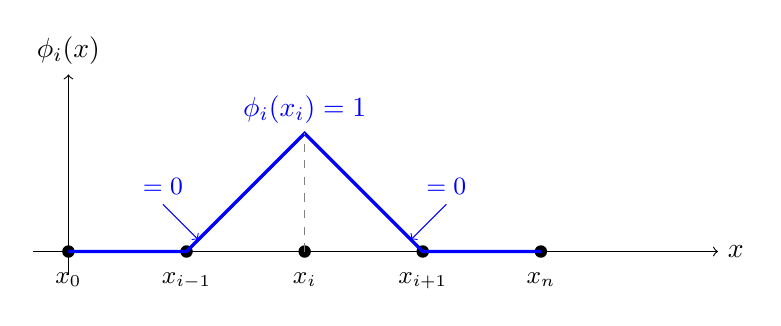
\begin{tikzpicture}[scale=1.5]
    % 坐标轴
    \draw[->] (-0.3,0) -- (5.5,0) node[right] {$x$};
    \draw[->] (0,-0.2) -- (0,1.5) node[above] {$\phi_i(x)$};
    
    % 网格节点
    \foreach \x/\lab in {0/$x_0$, 1/$x_{i-1}$, 2/$x_i$, 3/$x_{i+1}$, 4/$x_n$} {
        \fill (\x,0) circle (1.5pt);
        \node[below] at (\x,-0.1) {\small \lab};
    }
    
    % 形函数 φ_i
    \draw[very thick, blue] (0,0) -- (1,0) -- (2,1) -- (3,0) -- (4,0);
    
    % 标注
    \node[blue, above] at (2,1) {$\phi_i(x_i) = 1$};
    \draw[blue, <-] (1.1,0.1) -- (0.8,0.4) node[above] {\small $= 0$};
    \draw[blue, <-] (2.9,0.1) -- (3.2,0.4) node[above] {\small $= 0$};
    
    % 帐篷形状说明
    \draw[dashed, gray] (2,0) -- (2,1);
\end{tikzpicture}
\caption{帐篷函数 $\phi_i(x)$：在节点 $x_i$ 处等于 1，在相邻节点处等于 0，中间线性过渡}
\end{figure}

\paragraph{形函数的关键性质}

\begin{equation}
\phi_i(x_j) = \delta_{ij} = \begin{cases} 1, & i = j \\ 0, & i \neq j \end{cases}
\end{equation}

这个性质保证了：\textbf{系数 $U_i$ 恰好等于节点 $x_i$ 处的近似解值}！

验证：
\[
u_h(x_i) = \sum_j U_j \phi_j(x_i) = \sum_j U_j \delta_{ji} = U_i
\]

\subsection{从弱形式到线性方程组}

现在把近似解 $u_h = \sum_j U_j \phi_j$ 代入弱形式。

测试函数也用形函数：取 $v = \phi_i$（$i = 1, 2, \ldots, n$）

\paragraph{代入弱形式}

\[
\int_0^1 u_h' \cdot \phi_i' \, dx = \int_0^1 f \cdot \phi_i \, dx
\]

左边：
\[
\int_0^1 \left(\sum_j U_j \phi_j'\right) \phi_i' \, dx = \sum_j U_j \underbrace{\int_0^1 \phi_j' \phi_i' \, dx}_{K_{ij}}
\]

右边：
\[
\underbrace{\int_0^1 f \phi_i \, dx}_{F_i}
\]

于是得到：

\begin{keyformula}[title=有限元线性方程组]
\begin{equation}
\boxed{KU = F}
\end{equation}

其中：
\begin{itemize}
    \item $K_{ij} = \int_0^1 \phi_i'(x) \phi_j'(x) \, dx$ 是\textbf{刚度矩阵}的元素
    \item $F_i = \int_0^1 f(x) \phi_i(x) \, dx$ 是\textbf{载荷向量}的元素
    \item $U = (U_1, U_2, \ldots, U_n)^\top$ 是待求的\textbf{节点值向量}
\end{itemize}
\end{keyformula}

这就是有限元的核心方程！一个无限维的变分问题，变成了一个 $n \times n$ 的线性方程组。

% ------------------------------------------------------------------------------------
\section{刚度矩阵的计算}

\subsection{为什么叫"刚度矩阵"？}

"刚度"这个名字来自弹性力学。在弹簧系统中，$F = kx$，$k$ 是刚度——力与位移的比值。

在有限元中，$KU = F$ 说的是：\textbf{节点力 = 刚度矩阵 $\times$ 节点位移}。

$K_{ij}$ 的物理意义：给节点 $j$ 一个单位位移，节点 $i$ 受到多大的力？

\subsection{刚度矩阵的结构}

让我们计算刚度矩阵的元素 $K_{ij} = \int_0^1 \phi_i' \phi_j' dx$。

\paragraph{关键观察}

帐篷函数 $\phi_i$ 只在 $[x_{i-1}, x_{i+1}]$ 区间内非零（\textbf{局部支撑}）。

因此：
\begin{itemize}
    \item 如果 $|i - j| > 1$（节点不相邻），$\phi_i$ 和 $\phi_j$ 的支撑不重叠 $\Rightarrow$ $K_{ij} = 0$
    \item 只有 $|i - j| \leq 1$（相邻或相同节点）时，$K_{ij} \neq 0$
\end{itemize}

这导致刚度矩阵是\textbf{稀疏的三对角矩阵}！

\begin{figure}[h]
\centering
\begin{tikzpicture}[scale=0.6]
    % 画一个 5x5 的矩阵
    \draw[gray] (0,0) grid (5,5);
    
    % 填充非零元素
    % 主对角线
    \foreach \i in {0,...,4} {
        \fill[blue!60] (\i,4-\i) rectangle ++(1,1);
    }
    % 上下对角线
    \foreach \i in {0,...,3} {
        \fill[blue!30] (\i+1,4-\i) rectangle ++(1,1);
        \fill[blue!30] (\i,3-\i) rectangle ++(1,1);
    }
    
    % 标注
    \node at (2.5,-1) {三对角矩阵};
    \node[right] at (5.5,4.5) {\small $K_{11}$};
    \node[right] at (5.5,3.5) {\small $K_{22}$};
    \draw[->] (5.3,2.5) -- (4.2,2.5);
    \node[right] at (5.5,2.5) {\small 对角线};
\end{tikzpicture}
\caption{一维有限元的刚度矩阵是三对角的：只有相邻节点之间有耦合}
\end{figure}

\subsection{具体计算刚度矩阵元素}

设网格是均匀的，步长为 $h = \frac{1}{N}$，节点为 $x_k = kh$（$k = 0, 1, \ldots, N$）。

\paragraph{情况1：对角线元素 $K_{ii}$（$i$ 和自己的耦合）}

$\phi_i$ 在 $[x_{i-1}, x_i]$ 上斜率为 $+\frac{1}{h}$，在 $[x_i, x_{i+1}]$ 上斜率为 $-\frac{1}{h}$。

\begin{figure}[h]
\centering
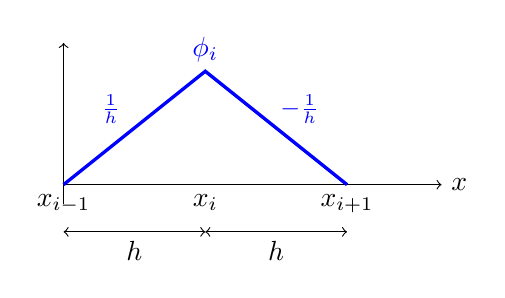
\begin{tikzpicture}[scale=1.2]
    \draw[->] (0,0) -- (4,0) node[right] {$x$};
    \draw[->] (0,-0.2) -- (0,1.5);
    
    % 形函数
    \draw[very thick, blue] (0,0) -- (1.5,1.2) -- (3,0);
    \node[blue, above] at (1.5,1.2) {$\phi_i$};
    
    % 斜率标注
    \node[blue] at (0.5,0.8) {\small $\frac{1}{h}$};
    \node[blue] at (2.5,0.8) {\small $-\frac{1}{h}$};
    
    % 节点
    \node[below] at (0,0) {$x_{i-1}$};
    \node[below] at (1.5,0) {$x_i$};
    \node[below] at (3,0) {$x_{i+1}$};
    
    % 区间标注
    \draw[<->] (0,-0.5) -- (1.5,-0.5) node[midway, below] {$h$};
    \draw[<->] (1.5,-0.5) -- (3,-0.5) node[midway, below] {$h$};
\end{tikzpicture}
\end{figure}

\begin{align}
K_{ii} &= \int_{x_{i-1}}^{x_{i+1}} (\phi_i')^2 \, dx \\
&= \int_{x_{i-1}}^{x_i} \left(\frac{1}{h}\right)^2 dx + \int_{x_i}^{x_{i+1}} \left(-\frac{1}{h}\right)^2 dx \\
&= \frac{1}{h^2} \cdot h + \frac{1}{h^2} \cdot h = \frac{2}{h}
\end{align}

\paragraph{情况2：相邻元素 $K_{i,i+1}$（相邻节点的耦合）}

$\phi_i$ 和 $\phi_{i+1}$ 只在 $[x_i, x_{i+1}]$ 上同时非零。

\begin{figure}[h]
\centering
\begin{tikzpicture}[scale=1.8]
    % 坐标轴
    \draw[->] (-0.3,0) -- (4.5,0) node[right] {$x$};
    \draw[->] (0,-0.2) -- (0,1.5) node[above] {};
    
    % 网格节点
    \foreach \x/\lab in {0/$x_{i-1}$, 1.5/$x_i$, 3/$x_{i+1}$, 4.5/$x_{i+2}$} {
        \fill (\x,0) circle (1.5pt);
    }
    \node[below] at (0,-0.1) {\small $x_{i-1}$};
    \node[below] at (1.5,-0.1) {\small $x_i$};
    \node[below] at (3,-0.1) {\small $x_{i+1}$};
    \node[below] at (4.2,-0.1) {\small $x_{i+2}$};
    
    % 形函数 φ_i (蓝色)
    \draw[very thick, blue] (0,0) -- (1.5,1.2) -- (3,0);
    \node[blue, above left] at (1.5,1.2) {$\phi_i$};
    
    % 形函数 φ_{i+1} (红色)
    \draw[very thick, red] (1.5,0) -- (3,1.2) -- (4.2,0);
    \node[red, above right] at (3,1.2) {$\phi_{i+1}$};
    
    % 重叠区域高亮
    \fill[purple, opacity=0.15] (1.5,0) -- (3,0) -- (3,1.2) -- (1.5,1.2) -- cycle;
    \fill[purple, opacity=0.15] (1.5,0) -- (1.5,1.2) -- (3,0) -- cycle;
    
    % 实际重叠的三角形区域（两个函数都非零的地方）
    \fill[green, opacity=0.2] (1.5,0) -- (2.25,0.6) -- (3,0) -- cycle;
    
    % 斜率标注
    \draw[blue, thick, ->] (2,0.4) -- (2.4,0.08);
    \node[blue] at (2.5,0.5) {\small $\phi_i' = -\dfrac{1}{h}$};
    
    \draw[red, thick, ->] (2.2,0.25) -- (2.6,0.57);
    \node[red] at (1.8,0.9) {\small $\phi_{i+1}' = +\dfrac{1}{h}$};
    
    % 区间标注
    \draw[<->, thick, purple] (1.5,-0.4) -- (3,-0.4);
    \node[purple, below] at (2.25,-0.4) {\small 重叠区间 $[x_i, x_{i+1}]$};
    
    % h 标注
    \draw[<->] (1.5,-0.7) -- (3,-0.7);
    \node at (2.25,-0.9) {\small $h$};
\end{tikzpicture}
\caption{相邻形函数 $\phi_i$ 和 $\phi_{i+1}$ 在区间 $[x_i, x_{i+1}]$ 上重叠。在此区间内，$\phi_i$ 下降（斜率 $-1/h$），$\phi_{i+1}$ 上升（斜率 $+1/h$），导致 $K_{i,i+1} < 0$。}
\end{figure}

在重叠区间 $[x_i, x_{i+1}]$ 上：
\begin{itemize}
    \item $\phi_i$ 从 1 下降到 0，斜率 $\phi_i' = -\dfrac{1}{h}$
    \item $\phi_{i+1}$ 从 0 上升到 1，斜率 $\phi_{i+1}' = +\dfrac{1}{h}$
\end{itemize}

\begin{align}
K_{i,i+1} &= \int_{x_i}^{x_{i+1}} \phi_i' \cdot \phi_{i+1}' \, dx \\
&= \int_{x_i}^{x_{i+1}} \left(-\frac{1}{h}\right) \cdot \left(+\frac{1}{h}\right) dx \\
&= -\frac{1}{h^2} \cdot h = \boxed{-\frac{1}{h}}
\end{align}

\begin{physicalmeaning}
$K_{i,i+1} < 0$ 的物理意义：相邻节点之间是\textbf{负耦合}。

用弹簧网络的比喻：节点 $i$ 和 $i+1$ 之间连着一根弹簧。当节点 $i$ 向上移动时，弹簧会把节点 $i+1$ 也往上拉——这就是负刚度系数的来源。

对角线元素 $K_{ii} = \frac{2}{h} > 0$（正刚度），非对角线元素 $K_{i,i+1} = -\frac{1}{h} < 0$（负耦合），这种结构保证了刚度矩阵的正定性。
\end{physicalmeaning}

\paragraph{情况3：不相邻元素 $K_{ij}$（$|i-j| > 1$）}

$\phi_i$ 和 $\phi_j$ 的支撑不重叠，所以：
\[
K_{ij} = \int_0^1 \phi_i' \phi_j' dx = 0
\]

\subsection{刚度矩阵的完整形式}

综合以上，对于均匀网格，内部节点（$i = 1, 2, \ldots, N-1$）的刚度矩阵是：

\begin{equation}
K = \frac{1}{h}
\begin{pmatrix}
2 & -1 & 0 & \cdots & 0 \\
-1 & 2 & -1 & \cdots & 0 \\
0 & -1 & 2 & \cdots & 0 \\
\vdots & & \ddots & \ddots & \vdots \\
0 & 0 & \cdots & -1 & 2
\end{pmatrix}
\end{equation}

\begin{insightbox}
\textbf{惊人的巧合}：对于均匀网格，有限元得到的矩阵 $\frac{1}{h}[-1, 2, -1]$ 与\textbf{二阶中心差分}完全相同！

但有限元的优势在于：
\begin{itemize}
    \item 可以处理非均匀网格
    \item 可以处理复杂几何（二维、三维）
    \item 有坚实的数学理论保证收敛
\end{itemize}
\end{insightbox}

% ------------------------------------------------------------------------------------
\section{完整例题：手算有限元}

让我们完整地手算一个例子，加深理解。

\subsection{问题设定}

求解：
\[
-u''(x) = 1, \quad x \in (0, 1), \quad u(0) = u(1) = 0
\]

使用 4 个单元（5 个节点），步长 $h = 0.25$。
\begin{figure}[h]
\centering
\begin{tikzpicture}[scale=1.2]
    % ===== 上半部分：各个加权形函数 =====
    \node[anchor=south] at (2,4.8) {\textbf{各个加权形函数}};
    
    % 坐标轴（上）
    \draw[->] (-0.3,3) -- (4.5,3) node[right] {\small $x$};
    \draw[->] (0,2.8) -- (0,4.7);
    
    % 节点位置
    \foreach \i in {0,1,2,3,4} {
        \fill (\i,3) circle (1.5pt);
    }
    
    % U_1 φ_1 (蓝色) - 高度 0.09375 × 10 = 0.9375 (放大显示)
    \draw[very thick, blue] (0,3) -- (1,3.75) -- (2,3);
    \node[blue, right] at (1.1,3.85) {\small $U_1\phi_1$};
    
    % U_2 φ_2 (红色) - 高度 0.125 × 10 = 1.25
    \draw[very thick, red] (1,3) -- (2,4) -- (3,3);
    \node[red, above] at (2,4.05) {\small $U_2\phi_2$};
    
    % U_3 φ_3 (green) - 高度 0.09375 × 10 = 0.9375
    \draw[very thick, green!60!black] (2,3) -- (3,3.75) -- (4,3);
    \node[green!60!black, left] at (2.9,3.85) {\small $U_3\phi_3$};
    
    % 节点值标注
    \node[blue, below] at (1,2.9) {\scriptsize $U_1$};
    \node[red, below] at (2,2.9) {\scriptsize $U_2$};
    \node[green!60!black, below] at (3,2.9) {\scriptsize $U_3$};
    
    % ===== 加号 =====
    \node at (2,2.3) {\Large $\Downarrow$ \normalsize 叠加};
    
    % ===== 下半部分：叠加结果 =====
    \node[anchor=south] at (2,1.3) {\textbf{近似解 $u_h(x) = \sum_{j=1}^{3} U_j \phi_j(x)$}};
    
    % 坐标轴（下）
    \draw[->] (-0.3,0) -- (4.5,0) node[right] {\small $x$};
    \draw[->] (0,-0.2) -- (0,1.3);
    
    % 节点
    \foreach \i in {0,1,2,3,4} {
        \fill (\i,0) circle (1.5pt);
    }
    \node[below] at (0,-0.1) {\scriptsize $0$};
    \node[below] at (4,-0.1) {\scriptsize $1$};
    
    % 叠加后的分段线性函数 (紫色粗线)
    \draw[very thick, purple] (0,0) -- (1,0.75) -- (2,1) -- (3,0.75) -- (4,0);
    
    % 节点值标注
    \fill[purple] (1,0.75) circle (2pt);
    \fill[purple] (2,1) circle (2pt);
    \fill[purple] (3,0.75) circle (2pt);
    \node[purple, above left] at (1,0.75) {\small $U_1$};
    \node[purple, above] at (2,1.05) {\small $U_2$};
    \node[purple, above right] at (3,0.75) {\small $U_3$};
    
    % 精确解（虚线）
    \draw[dashed, gray, thick, domain=0:4, samples=50] plot (\x, {(\x/4)*(1-\x/4)*4});
    \node[gray, right] at (4.2,0.5) {\small 精确解};
    
    % 边界条件
    \fill[blue] (0,0) circle (2pt);
    \fill[blue] (4,0) circle (2pt);
    \node[blue, above left] at (0,0.1) {\scriptsize $U_0=0$};
    \node[blue, above right] at (4,0.1) {\scriptsize $U_4=0$};
\end{tikzpicture}
\caption{有限元近似解的构造：$u_h(x) = U_1\phi_1(x) + U_2\phi_2(x) + U_3\phi_3(x)$。每个形函数 $\phi_j$ 在节点 $j$ 处取值为 1，乘以节点值 $U_j$ 后叠加得到分段线性的近似解。灰色虚线为精确解 $u(x) = \frac{x(1-x)}{2}$。}
\end{figure}

\begin{insightbox}{形函数的"插值"本质}
形函数的关键性质是 $\phi_i(x_j) = \delta_{ij}$（在自己的节点上等于1，在其他节点上等于0）。

这意味着：
\[
u_h(x_j) = \sum_{k=1}^{n} U_k \phi_k(x_j) = \sum_{k=1}^{n} U_k \delta_{kj} = U_j
\]

即：\textbf{近似解在节点处的值恰好等于我们要求的未知量 $U_j$}！

形函数的作用就是在节点之间进行\textbf{线性插值}，把离散的节点值"连接"成连续函数。
\end{insightbox}

\subsection{第一步：组装刚度矩阵}

对于内部 3 个自由度，刚度矩阵是 $3 \times 3$：

\[
K = \frac{1}{h}
\begin{pmatrix}
2 & -1 & 0 \\
-1 & 2 & -1 \\
0 & -1 & 2
\end{pmatrix}
= \frac{1}{0.25}
\begin{pmatrix}
2 & -1 & 0 \\
-1 & 2 & -1 \\
0 & -1 & 2
\end{pmatrix}
=
\begin{pmatrix}
8 & -4 & 0 \\
-4 & 8 & -4 \\
0 & -4 & 8
\end{pmatrix}
\]

\subsection{第二步：计算载荷向量}

对于 $f(x) = 1$，载荷向量的第 $i$ 个分量为：
\[
F_i = \int_0^1 1 \cdot \phi_i(x) \, dx
\]

$\phi_i$ 是一个"帐篷"，底边宽 $2h$，高度为 1，面积为：
\[
F_i = \frac{1}{2} \times 2h \times 1 = h = 0.25
\]

（边界节点的形函数只有半个帐篷，但它们对应 $U_0 = U_4 = 0$，不参与方程。）

载荷向量：
\[
F = \begin{pmatrix} 0.25 \\ 0.25 \\ 0.25 \end{pmatrix}
\]

\subsection{第三步：求解线性方程组}

现在求解：
\[
\begin{pmatrix}
8 & -4 & 0 \\
-4 & 8 & -4 \\
0 & -4 & 8
\end{pmatrix}
\begin{pmatrix} U_1 \\ U_2 \\ U_3 \end{pmatrix}
=
\begin{pmatrix} 0.25 \\ 0.25 \\ 0.25 \end{pmatrix}
\]

\paragraph{用高斯消元法求解}

第一个方程：$8U_1 - 4U_2 = 0.25$

第二个方程加上第一个方程的 $\frac{1}{2}$ 倍：
\[
(-4 + 4)U_1 + (8 - 2)U_2 - 4U_3 = 0.25 + 0.125 \quad \Rightarrow \quad 6U_2 - 4U_3 = 0.375
\]

第三个方程加上新的第二个方程的 $\frac{2}{3}$ 倍：
\[
(8 - \frac{8}{3})U_3 = 0.25 + 0.25 \quad \Rightarrow \quad \frac{16}{3}U_3 = 0.5 \quad \Rightarrow \quad U_3 = 0.09375
\]

回代：
\[
U_2 = \frac{0.375 + 4 \times 0.09375}{6} = \frac{0.75}{6} = 0.125
\]
\[
U_1 = \frac{0.25 + 4 \times 0.125}{8} = \frac{0.75}{8} = 0.09375
\]

\subsection{第四步：检验结果}

有限元解：
\[
U_1 = U_3 = 0.09375, \quad U_2 = 0.125
\]

精确解 $u(x) = \frac{x(1-x)}{2}$ 在节点处的值：
\[
u(0.25) = \frac{0.25 \times 0.75}{2} = 0.09375
\]
\[
u(0.5) = \frac{0.5 \times 0.5}{2} = 0.125
\]
\[
u(0.75) = \frac{0.75 \times 0.25}{2} = 0.09375
\]

\textbf{有限元解在节点处恰好等于精确解！}

\begin{figure}[h]
\centering
\begin{tikzpicture}[x=6cm, y=15cm]
    % 坐标轴
    \draw[->] (-0.05,0) -- (1.15,0) node[right] {$x$};
    \draw[->] (0,-0.01) -- (0,0.15) node[above] {$u(x)$};
    
    % 刻度
    \foreach \x in {0, 0.25, 0.5, 0.75, 1} {
        \draw (\x,0) -- (\x,-0.005);
        \node[below] at (\x,-0.005) {\scriptsize $\x$};
    }
    \foreach \y in {0, 0.05, 0.1} {
        \draw (0,\y) -- (-0.02,\y);
        \node[left] at (-0.02,\y) {\scriptsize $\y$};
    }
    
    % 精确解
    \draw[thick, gray, dashed, domain=0:1, samples=50] plot (\x, {0.5*\x*(1-\x)});
    \node[gray] at (0.85,0.11) {\small 精确解};
    
    % 有限元解
    \draw[very thick, blue] (0,0) -- (0.25,0.09375) -- (0.5,0.125) -- (0.75,0.09375) -- (1,0);
    \node[blue] at (0.15,0.06) {\small $u_h(x)$};
    
    % 节点
    \fill[red] (0.25,0.09375) circle (2pt);
    \fill[red] (0.5,0.125) circle (2pt);
    \fill[red] (0.75,0.09375) circle (2pt);
\end{tikzpicture}
\caption{有限元解（蓝色折线）与精确解（灰色虚线）的对比}
\end{figure}

\begin{insightbox}
\textbf{超收敛现象}：对于一维问题和线性形函数，有限元解在节点处恰好等于精确解！

这是一维问题的特殊性质。在二维、三维问题中，有限元解在节点处通常只是近似值，但仍然是"最优"的（在能量范数意义下）。
\end{insightbox}

% ------------------------------------------------------------------------------------
\section{单元组装：从局部到整体}

在实际计算中，我们不直接计算整体刚度矩阵。而是：
\begin{enumerate}
    \item 在每个小\textbf{单元}上计算\textbf{单元刚度矩阵}
    \item 把所有单元刚度矩阵\textbf{组装}成整体刚度矩阵
\end{enumerate}

这种"分而治之"的策略使有限元方法非常灵活——可以处理不规则网格、不同类型的单元混合等。

\subsection{单元刚度矩阵}

对于一维线性单元（两个节点），单元刚度矩阵是 $2 \times 2$ 的：

\begin{keyformula}[title=一维线性单元刚度矩阵]
\begin{equation}
K^e = \frac{1}{h}
\begin{pmatrix}
1 & -1 \\
-1 & 1
\end{pmatrix}
\end{equation}

行和列分别对应单元的左节点和右节点。
\end{keyformula}

\paragraph{推导}

设单元长度为 $h$，两端节点为 $x_L$ 和 $x_R$。

单元内的两个形函数：
\[
N_L(x) = \frac{x_R - x}{h}, \quad N_R(x) = \frac{x - x_L}{h}
\]

它们的导数：
\[
N_L' = -\frac{1}{h}, \quad N_R' = \frac{1}{h}
\]

单元刚度矩阵的元素：
\[
K^e_{LL} = \int_{x_L}^{x_R} (N_L')^2 dx = \frac{1}{h^2} \cdot h = \frac{1}{h}
\]
\[
K^e_{LR} = \int_{x_L}^{x_R} N_L' N_R' dx = -\frac{1}{h^2} \cdot h = -\frac{1}{h}
\]
\[
K^e_{RR} = \int_{x_L}^{x_R} (N_R')^2 dx = \frac{1}{h^2} \cdot h = \frac{1}{h}
\]

\subsection{组装过程}

组装的规则很简单：把每个单元刚度矩阵"放入"整体矩阵的对应位置，重叠处累加。

\begin{figure}[h]
\centering
\begin{tikzpicture}[scale=0.6]
    % 单元1矩阵（用数学矩阵表示，不用tikz框）
    \node[anchor=east] at (-2,6) {\small 单元1 (节点0-1):};
    \node at (0,6) {$\begin{pmatrix} \frac{1}{h} & -\frac{1}{h} \\[3pt] -\frac{1}{h} & \frac{1}{h} \end{pmatrix}$};

    % 箭头指向蓝色区域
    \draw[->, thick, blue!70] (1.8,6) -- (4.2,4.5);

    % 单元2矩阵
    \node[anchor=east] at (-2,2) {\small 单元2 (节点1-2):};
    \node at (0,2) {$\begin{pmatrix} \frac{1}{h} & -\frac{1}{h} \\[3pt] -\frac{1}{h} & \frac{1}{h} \end{pmatrix}$};

    % 箭头指向橙色区域
    \draw[->, thick, orange!80] (1.8,2) -- (5.2,2.5);

    % 整体矩阵框架
    \draw[thick] (4,0) grid (9,5);

    % 填充蓝色区域（单元1贡献：节点0,1）
    \fill[blue!25] (4,4) rectangle (5,5);
    \fill[blue!25] (5,4) rectangle (6,5);
    \fill[blue!25] (4,3) rectangle (5,4);
    \fill[blue!25] (5,3) rectangle (6,4);

    % 填充橙色区域（单元2贡献：节点1,2）
    \fill[orange!25] (5,3) rectangle (6,4);
    \fill[orange!25] (6,3) rectangle (7,4);
    \fill[orange!25] (5,2) rectangle (6,3);
    \fill[orange!25] (6,2) rectangle (7,3);

    % 重叠处（节点1的对角元）用红色标出
    \fill[red!40] (5,3) rectangle (6,4);
    \node[font=\footnotesize] at (5.5,3.5) {$\frac{2}{h}$};

    % 列标签（在矩阵上方）
    \foreach \i in {0,...,4} {
        \node[above, font=\scriptsize] at (4.5+\i,5.1) {\i};
    }
    % 行标签（在矩阵左侧）
    \foreach \i in {0,...,4} {
        \node[left, font=\scriptsize] at (3.9,4.5-\i) {\i};
    }

    % 整体矩阵标题
    \node[above] at (6.5,5.5) {\small 整体刚度矩阵 $K$};

    % 说明文字
    \node at (6.5,-0.8) {\small 重叠处累加：$\frac{1}{h} + \frac{1}{h} = \frac{2}{h}$};
\end{tikzpicture}
\caption{组装过程示意：单元矩阵放入整体矩阵对应位置，重叠处累加}
\end{figure}

\begin{physicalmeaning}
\textbf{组装的物理意义}：

\begin{itemize}
    \item 对角线元素 $K_{ii}$ 累加了所有与节点 $i$ 相连的单元贡献——节点的"总刚度"
    \item 非对角线元素 $K_{ij}$ 只来自同时包含 $i$ 和 $j$ 的单元——节点间的"耦合"
\end{itemize}

就像一个弹簧网络：每个节点的总刚度是连接它的所有弹簧刚度之和。
\end{physicalmeaning}

% ------------------------------------------------------------------------------------
\section{边界条件处理}

\subsection{Dirichlet 边界条件（固定值）}

我们的例子中，$u(0) = u(1) = 0$ 是 Dirichlet 边界条件——边界上的值是固定的。

\paragraph{处理方法1：直接消去}

既然 $U_0 = U_4 = 0$ 是已知的，就从方程组中删去这两个未知量，只求解内部节点。

这就是我们上面手算例子用的方法。

\paragraph{处理方法2：大数法（罚函数）}

把对角线元素改成一个很大的数，对应的载荷也相应修改：

\[
K_{00} \leftarrow 10^{20}, \quad F_0 \leftarrow 10^{20} \times g_0
\]

其中 $g_0$ 是边界值。这样方程 $10^{20} U_0 = 10^{20} g_0$ 就强制 $U_0 \approx g_0$。

\textbf{优点}：不改变矩阵结构，易于编程

\textbf{缺点}：矩阵条件数变差

\subsection{Neumann 边界条件（给定导数）}

如果边界条件是 $u'(1) = q$（给定热流），这是 Neumann 边界条件。

Neumann 条件在弱形式中\textbf{自然满足}——它会贡献到载荷向量：
\[
F_n \leftarrow F_n + q
\]

\subsection{拉格朗日乘子法}

和第1章一样，我们也可以用拉格朗日乘子处理边界条件！

把边界条件 $u(0) = g$ 看作约束，引入乘子 $\lambda$：
\[
\mathcal{L}[u, \lambda] = J[u] + \lambda(u(0) - g)
\]

这导出一个\textbf{鞍点问题}：
\[
\begin{pmatrix}
K & B^\top \\
B & 0
\end{pmatrix}
\begin{pmatrix}
U \\
\lambda
\end{pmatrix}
=
\begin{pmatrix}
F \\
g
\end{pmatrix}
\]

\begin{physicalmeaning}
$\lambda$ 的物理意义是边界处的\textbf{法向通量}：
\begin{itemize}
    \item 热传导：$\lambda$ = 热流密度（W/m²）
    \item 弹性力学：$\lambda$ = 边界反力（N）
\end{itemize}

这与第5章力学中的约束力完全对应——边界条件本质上也是约束！
\end{physicalmeaning}

% ------------------------------------------------------------------------------------
\section{误差分析与收敛性}

\subsection{误差的来源}

有限元解 $u_h$ 与精确解 $u$ 之间有误差。误差来自哪里？

\begin{itemize}
    \item \textbf{离散化误差}：用有限维空间逼近无限维空间
    \item \textbf{插值误差}：用分片多项式逼近光滑函数
\end{itemize}

\subsection{误差估计}

对于线性形函数，误差有如下估计：

\begin{keytheorem}[title=有限元误差估计]
设 $u$ 是精确解，$u_h$ 是线性有限元解，$h$ 是网格步长。则：

\textbf{能量范数误差}：
\[
\|u' - u_h'\|_{L^2} \leq Ch \|u''\|_{L^2}
\]

\textbf{$L^2$ 范数误差}：
\[
\|u - u_h\|_{L^2} \leq Ch^2 \|u''\|_{L^2}
\]

其中 $C$ 是与 $h$ 无关的常数。
\end{keytheorem}

\paragraph{含义}

\begin{itemize}
    \item 网格加密一倍（$h \to h/2$），导数误差减半，函数值误差减到 $\frac{1}{4}$
    \item 线性元的收敛阶是 $O(h)$（能量范数）或 $O(h^2)$（$L^2$ 范数）
    \item 用更高阶的多项式（如二次元、三次元），可以获得更高的收敛阶
\end{itemize}

\subsection{数值验证}

让我们用不同的网格密度求解 $-u'' = 1$，验证收敛性：

\begin{center}
\begin{tabular}{c|c|c|c}
\toprule
单元数 $N$ & 步长 $h$ & 最大误差 & 误差比 \\
\midrule
4 & 0.25 & $7.8 \times 10^{-3}$ & -- \\
8 & 0.125 & $2.0 \times 10^{-3}$ & 3.9 \\
16 & 0.0625 & $4.9 \times 10^{-4}$ & 4.1 \\
32 & 0.03125 & $1.2 \times 10^{-4}$ & 4.1 \\
\bottomrule
\end{tabular}
\end{center}

每次加密一倍，误差减少到约 $\frac{1}{4}$——符合 $O(h^2)$ 的理论预测！

% ------------------------------------------------------------------------------------
\section{二维问题简介}

\subsection{从一维到二维}

一维的思想可以自然推广到二维。

\textbf{二维 Poisson 方程}：
\[
-\nabla^2 u = -\left(\frac{\partial^2 u}{\partial x^2} + \frac{\partial^2 u}{\partial y^2}\right) = f \quad \text{in } \Omega
\]

\textbf{弱形式}：
\[
\int_\Omega \nabla u \cdot \nabla v \, dA = \int_\Omega fv \, dA
\]

\textbf{离散化}：把区域 $\Omega$ 剖分成三角形或四边形单元。

\begin{figure}[h]
\centering
\begin{tikzpicture}[scale=0.8]
    % 区域
    \draw[thick] (0,0) -- (4,0) -- (4,3) -- (0,3) -- cycle;
    
    % 三角形网格
    \foreach \x in {0,1,...,4} {
        \foreach \y in {0,1,2,3} {
            \fill (\x,\y) circle (1.5pt);
        }
    }
    
    % 画一些三角形
    \draw[gray] (0,0) -- (1,1) -- (0,1) -- cycle;
    \draw[gray] (0,0) -- (1,0) -- (1,1) -- cycle;
    \draw[gray] (1,0) -- (2,1) -- (1,1) -- cycle;
    \draw[gray] (1,0) -- (2,0) -- (2,1) -- cycle;
    \draw[gray] (2,0) -- (3,1) -- (2,1) -- cycle;
    \draw[gray] (2,0) -- (3,0) -- (3,1) -- cycle;
    \draw[gray] (3,0) -- (4,1) -- (3,1) -- cycle;
    \draw[gray] (3,0) -- (4,0) -- (4,1) -- cycle;
    
    \draw[gray] (0,1) -- (1,2) -- (0,2) -- cycle;
    \draw[gray] (0,1) -- (1,1) -- (1,2) -- cycle;
    \draw[gray] (1,1) -- (2,2) -- (1,2) -- cycle;
    \draw[gray] (1,1) -- (2,1) -- (2,2) -- cycle;
    \draw[gray] (2,1) -- (3,2) -- (2,2) -- cycle;
    \draw[gray] (2,1) -- (3,1) -- (3,2) -- cycle;
    \draw[gray] (3,1) -- (4,2) -- (3,2) -- cycle;
    \draw[gray] (3,1) -- (4,1) -- (4,2) -- cycle;
    
    \draw[gray] (0,2) -- (1,3) -- (0,3) -- cycle;
    \draw[gray] (0,2) -- (1,2) -- (1,3) -- cycle;
    \draw[gray] (1,2) -- (2,3) -- (1,3) -- cycle;
    \draw[gray] (1,2) -- (2,2) -- (2,3) -- cycle;
    \draw[gray] (2,2) -- (3,3) -- (2,3) -- cycle;
    \draw[gray] (2,2) -- (3,2) -- (3,3) -- cycle;
    \draw[gray] (3,2) -- (4,3) -- (3,3) -- cycle;
    \draw[gray] (3,2) -- (4,2) -- (4,3) -- cycle;
    
    % 标注
    \node at (2,-0.8) {三角形网格剖分};
\end{tikzpicture}
\caption{二维有限元：区域被剖分成三角形单元}
\end{figure}

\subsection{三角形单元}

最简单的二维单元是线性三角形单元。每个三角形有 3 个节点，单元内的近似解是：
\[
u_h(x, y) = U_1 N_1(x,y) + U_2 N_2(x,y) + U_3 N_3(x,y)
\]

其中 $N_i$ 是线性形函数，满足 $N_i(x_j, y_j) = \delta_{ij}$。

\paragraph{单元刚度矩阵}

三角形单元的刚度矩阵是 $3 \times 3$：
\[
K^e_{ij} = \int_{\text{三角形}} \nabla N_i \cdot \nabla N_j \, dA
\]

由于 $N_i$ 是线性函数，$\nabla N_i$ 是常向量，积分很容易计算。

\subsection{刚度矩阵的稀疏性}

二维问题的刚度矩阵仍然是稀疏的——只有相邻节点之间有耦合。

但稀疏结构更复杂：不再是三对角，而是\textbf{带状稀疏}矩阵。

\begin{figure}[h]
\centering
\begin{tikzpicture}[scale=0.08]
    % 画一个稀疏矩阵的样子
    \draw[gray] (0,0) rectangle (50,50);
    
    % 用随机点表示非零元素
    \foreach \i in {0,...,49} {
        \fill[blue] (\i,49-\i) circle (1);
        \pgfmathsetmacro{\jone}{int(\i+1)}
        \pgfmathsetmacro{\jtwo}{int(\i+2)}
        \pgfmathsetmacro{\jthree}{int(\i+5)}
        \pgfmathsetmacro{\jfour}{int(\i+6)}
        \ifnum\i<49
            \fill[blue!50] (\jone,49-\i) circle (0.8);
            \fill[blue!50] (\i,49-\jone) circle (0.8);
        \fi
        \ifnum\i<48
            \fill[blue!30] (\jtwo,49-\i) circle (0.6);
            \fill[blue!30] (\i,49-\jtwo) circle (0.6);
        \fi
        \ifnum\i<45
            \fill[blue!20] (\jthree,49-\i) circle (0.5);
            \fill[blue!20] (\i,49-\jthree) circle (0.5);
        \fi
    }
    
    \node at (25,-8) {\small 二维有限元的稀疏刚度矩阵};
\end{tikzpicture}
\end{figure}

% ------------------------------------------------------------------------------------
% ------------------------------------------------------------------------------------
\section{殊途同归：有限差分与有限元}

在继续深入之前，让我们回答一个常见问题：有限差分法（FDM）和有限元法（FEM）有什么区别？

\subsection{一维情况：完全等价}

考虑一维问题 $-u'' = f$，用 $N$ 个等距节点离散化。

\begin{figure}[h]
\centering
\begin{tikzpicture}[scale=1.2]
    % 左边：FDM
    \node[font=\bfseries] at (-3, 2) {有限差分 (FDM)};
    \draw[->] (-5, 0) -- (-1, 0) node[right] {$x$};
    \foreach \i in {0,1,2,3,4} {
        \fill (-5+\i, 0) circle (2pt);
        \node[below] at (-5+\i, -0.2) {\small $x_\i$};
    }
    % Taylor展开示意
    \draw[blue, thick, ->] (-3, 0.3) -- (-4, 0.3);
    \draw[blue, thick, ->] (-3, 0.3) -- (-2, 0.3);
    \node[blue, above] at (-3, 0.4) {\small Taylor展开};
    
    % 右边：FEM
    \node[font=\bfseries] at (3, 2) {有限元 (FEM)};
    \draw[->] (1, 0) -- (5, 0) node[right] {$x$};
    \foreach \i in {0,1,2,3,4} {
        \fill (1+\i, 0) circle (2pt);
    }
    % 形函数示意
    \draw[red, thick] (1,0) -- (2,0.8) -- (3,0);
    \draw[red, thick] (2,0) -- (3,0.8) -- (4,0);
    \node[red, above] at (3, 0.9) {\small 形函数};
\end{tikzpicture}
\caption{有限差分 vs 有限元的离散化方式}
\end{figure}

\vspace{0.3cm}
\noindent
\begin{minipage}[t]{0.48\textwidth}
\textbf{有限差分的推导}

出发点：Taylor展开近似导数
\[
-u''(x_i) \approx -\frac{u_{i+1} - 2u_i + u_{i-1}}{h^2}
\]

离散方程（第 $i$ 行）：
\[
\frac{-u_{i-1} + 2u_i - u_{i+1}}{h^2} = f_i
\]

系数：$\left[ -\frac{1}{h^2}, \; \frac{2}{h^2}, \; -\frac{1}{h^2} \right]$
\end{minipage}
\hfill
\begin{minipage}[t]{0.48\textwidth}
\textbf{有限元的推导}

出发点：弱形式 + 线性形函数
\[
K_{ij} = \int \phi_i' \phi_j' dx
\]

刚度矩阵（第 $i$ 行）：
\[
\frac{1}{h} [-1, \quad 2, \quad -1]
\]

方程：$\frac{-U_{i-1} + 2U_i - U_{i+1}}{h} = hf_i$
\end{minipage}

\vspace{0.5cm}
把FEM方程两边除以 $h$：
\[
\frac{-U_{i-1} + 2U_i - U_{i+1}}{h^2} = f_i
\]

\begin{insightbox}
在一维均匀网格上，线性有限元和中心差分给出\textbf{完全相同}的方程！

这不是巧合——两种方法从不同角度逼近了同一个物理问题。
\end{insightbox}



\subsection{二维情况：分道扬镳}

当问题升级到二维，两种方法开始展现本质区别。

\textbf{任务}：在圆形区域 $\Omega$ 上求解 $-\Delta u = f$。

\begin{figure}[h]
\centering
\begin{tikzpicture}[scale=1.8]
    % 左边：FDM
    \begin{scope}[xshift=-3cm]
        \node[font=\bfseries] at (0.5, 1.3) {有限差分};
        % 规则网格
        \draw[step=0.2, gray!30, thin] (0,0) grid (1.1,1.1);
        % 真实圆边界
        \draw[thick, red] (0,1) arc (90:0:1);
        % 锯齿逼近
        \draw[blue, thick]
            (0,1) -- (0.2,1) -- (0.2,0.8) --
            (0.4,0.8) -- (0.4,0.6) --
            (0.6,0.6) -- (0.6,0.4) --
            (0.8,0.4) -- (0.8,0.2) --
            (1.0,0.2) -- (1.0,0);
        % 五点差分模板
        \fill[blue] (0.6,0.4) circle (1pt);
        \foreach \dx/\dy in {0.2/0, -0.2/0, 0/0.2, 0/-0.2}{
            \draw[->, thick, blue!60] (0.6,0.4) -- +(\dx,\dy);
        }
        \node[red, font=\scriptsize] at (0.5, 1.15) {真实边界};
        \node[blue, font=\scriptsize] at (0.2, 0.5) {锯齿};
    \end{scope}
    
    % 右边：FEM
    \begin{scope}[xshift=1.5cm]
        \node[font=\bfseries] at (0.5, 1.3) {有限元};
        % 真实圆边界
        \draw[thick, red] (0,1) arc (90:0:1);
        % 三角剖分
        \coordinate (O) at (0,0);
        \coordinate (B) at (0,1);
        \coordinate (C) at (0.5,0.866);
        \coordinate (D) at (0.866,0.5);
        \coordinate (E) at (1,0);
        \coordinate (b) at (0,0.5);
        \coordinate (c) at (0.25,0.433);
        \coordinate (d) at (0.433,0.25);
        \coordinate (e) at (0.5,0);
        
        \draw[blue] (O) -- (b) -- (c) -- cycle;
        \draw[blue] (O) -- (c) -- (d) -- cycle;
        \draw[blue] (O) -- (d) -- (e) -- cycle;
        \draw[blue] (b) -- (B) -- (C) -- (c) -- cycle;
        \draw[blue] (c) -- (C) -- (D) -- (d) -- cycle;
        \draw[blue] (d) -- (D) -- (E) -- (e) -- cycle;
        
        % 边界节点
        \foreach \P in {B,C,D,E} {
            \fill[red] (\P) circle (1.5pt);
        }
        \node[blue, font=\scriptsize] at (0.5, 0.5) {三角形};
        \node[red, font=\scriptsize] at (0.7, 1.0) {节点在边界上};
    \end{scope}
\end{tikzpicture}
\caption{二维圆形区域的离散化：FDM用锯齿逼近边界，FEM可以精确贴合。}
\end{figure}

\begin{center}
\renewcommand{\arraystretch}{1.4}
\begin{tabular}{l|p{5cm}|p{5cm}}
\toprule
& \textbf{有限差分} & \textbf{有限元} \\
\midrule
网格类型 & 结构化（规则方格） & 非结构化（任意三角形） \\
边界处理 & 锯齿逼近，精度损失 & 节点直接在边界上 \\
复杂几何 & 困难（需要特殊处理） & 自然（只需网格生成） \\
实现难度 & 简单（数组索引） & 复杂（邻接关系） \\
适用场景 & 规则区域（图像、芯片） & 复杂几何（飞机、骨骼） \\
\bottomrule
\end{tabular}
\end{center}

\begin{physicalmeaning}
\textbf{为什么FEM统治了工程计算？}

现实世界的几何很少是规则的：飞机机翼是流线型的，人体骨骼是弯曲的，汽车车身是复杂曲面。

有限元的三角形/四面体网格可以\textbf{贴合任意几何形状}，这是它在工程中广泛应用的根本原因。

代价是：需要维护复杂的网格数据结构和邻接关系。
\end{physicalmeaning}

% ------------------------------------------------------------------------------------
\section{连续性的秘密}

\subsection{为什么要求连续？}

在前面的推导中，我们默默假设了 $u_h(x)$ 是连续的。但为什么？

\begin{figure}[h]
\centering
\begin{tikzpicture}[scale=1.2]
    % 上半部分：连续函数
    \begin{scope}[yshift=2cm]
        \draw[->] (0,0) -- (4,0) node[right] {$x$};
        \draw[->] (0,0) -- (0,1.5);
        \draw[blue, very thick] (0.5, 0.3) -- (2, 1.2) -- (3.5, 0.8);
        \node[blue] at (2, 1.5) {连续折线};
        \node[blue, align=center] at (5, 0.8) {导数有限 \\ 能量有限 $\checkmark$};
    \end{scope}
    
    % 下半部分：不连续函数
    \begin{scope}
        \draw[->] (0,0) -- (4,0) node[right] {$x$};
        \draw[->] (0,0) -- (0,1.5);
        \draw[red, very thick] (0.5, 0.3) -- (2, 1.2);
        \draw[red, very thick] (2, 0.4) -- (3.5, 0.8);
        \draw[red, dashed] (2, 0.4) -- (2, 1.2);
        \node[red] at (2.3, 0.8) {Jump!};
        \node[red, align=center] at (5, 0.8) {导数 $= \infty$ \\ 能量 $= \infty$ $\times$};
    \end{scope}
\end{tikzpicture}
\caption{连续性与能量的关系}
\end{figure}

\textbf{数学解释}：我们的弱形式包含梯度项 $\int |\nabla u|^2 dx$（能量）。

如果 $u$ 在某点有跳跃（不连续）：
\begin{itemize}
    \item 导数 $u'$ 在该点变成 Dirac $\delta$ 函数（无穷大）
    \item 能量 $\int (u')^2 dx = \int \delta^2 dx = \infty$
\end{itemize}

物理上，无穷大的能量是不允许的。

\begin{keyformula}[title=$C^0$ 连续性]
我们要求有限元解空间 $V_h \subset C^0(\Omega)$，即：

\textbf{函数值连续，但导数可以不连续}

换句话说：$u_h$ 可以"折"，但不能"断"。
\end{keyformula}

\subsection{线性单元如何保证连续？}

一个关键问题：我们只要求\textbf{节点值}相等，怎么能保证整条公共边上都连续？

\begin{figure}[h]
\centering
\begin{tikzpicture}[scale=1.5]
    % 两个三角形共享边
    \coordinate (N1) at (0,1);
    \coordinate (N2) at (0,-1);
    \coordinate (N3) at (-1.5, 0);
    \coordinate (N4) at (1.5, 0);
    
    \draw[fill=blue!10] (N1) -- (N2) -- (N3) -- cycle;
    \draw[fill=orange!10] (N1) -- (N2) -- (N4) -- cycle;
    
    % 共享边
    \draw[ultra thick, red] (N1) -- (N2);
    
    % 节点标注
    \node[above] at (N1) {$U_1$};
    \node[below] at (N2) {$U_2$};
    \node[left] at (N3) {$U_3$};
    \node[right] at (N4) {$U_4$};
    
    \node[blue] at (-0.7, 0) {单元 A};
    \node[orange] at (0.7, 0) {单元 B};
    
    % 边上的点
    \fill[black] (0, 0.3) circle (1.5pt) node[right] {$P$};
\end{tikzpicture}
\caption{两个三角形共享边 1-2}
\end{figure}

\textbf{几何证明}：

\begin{enumerate}
    \item 在三角形 A 内部，$u_h$ 是一个\textbf{平面}（线性函数）
    
    \item 这个平面在边 1-2 上截出一条\textbf{直线}
    
    \item 这条直线由两个端点值 $U_1$ 和 $U_2$ \textbf{唯一确定}（两点定一线！）
    
    \item 同样，三角形 B 在边 1-2 上也截出一条直线，也由 $U_1$ 和 $U_2$ 确定
    
    \item 两条直线端点相同 $\Rightarrow$ 两条直线重合！
\end{enumerate}

\begin{insightbox}
\textbf{线性单元连续性的关键}：两点确定一条直线。

只要共享节点的值相同，整条公共边就自动连续——就像\textbf{合页(Hinge)}一样严丝合缝。

这就是为什么线性单元只需要在顶点处设置自由度。
\end{insightbox}

\textbf{高阶单元怎么办？}

如果是二次单元，边上的函数是抛物线。两点定不了抛物线！

解决方案：在边的中点增加一个节点，三点定抛物线。

\begin{figure}[h]
\centering
\begin{tikzpicture}[scale=1.2]
    % 线性单元
    \begin{scope}
        \node[font=\bfseries] at (1, 1.8) {线性单元};
        \draw[thick] (0,0) -- (2,0) -- (1,1.5) -- cycle;
        \fill[blue] (0,0) circle (3pt);
        \fill[blue] (2,0) circle (3pt);
        \fill[blue] (1,1.5) circle (3pt);
        \node[below] at (1, -0.3) {3个节点};
    \end{scope}
    
    % 二次单元
    \begin{scope}[xshift=5cm]
        \node[font=\bfseries] at (1, 1.8) {二次单元};
        \draw[thick] (0,0) -- (2,0) -- (1,1.5) -- cycle;
        % 顶点
        \fill[blue] (0,0) circle (3pt);
        \fill[blue] (2,0) circle (3pt);
        \fill[blue] (1,1.5) circle (3pt);
        % 边中点
        \fill[red] (1,0) circle (3pt);
        \fill[red] (1.5,0.75) circle (3pt);
        \fill[red] (0.5,0.75) circle (3pt);
        \node[below] at (1, -0.3) {6个节点};
    \end{scope}
\end{tikzpicture}
\caption{线性单元（3节点）vs 二次单元（6节点）}
\end{figure}

\subsection{一维二次单元详解}

为了理解高阶单元，让我们先看最简单的情况：一维二次单元。

\begin{figure}[h]
\centering
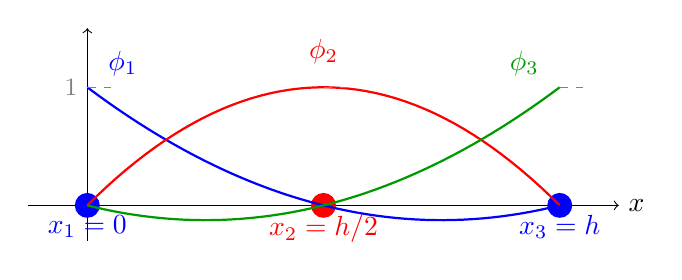
\begin{tikzpicture}[scale=1.5]
    % 坐标轴
    \draw[->] (-0.5, 0) -- (4.5, 0) node[right] {$x$};
    \draw[->] (0, -0.3) -- (0, 1.5);
    
    % 三个节点
    \fill[blue] (0, 0) circle (3pt) node[below] {$x_1 = 0$};
    \fill[red] (2, 0) circle (3pt) node[below] {$x_2 = h/2$};
    \fill[blue] (4, 0) circle (3pt) node[below] {$x_3 = h$};
    
    % 三个形函数
    % φ_1: 在x_1=1, 其他=0
    \draw[blue, thick, domain=0:4, samples=50] plot (\x, {((\x-2)*(\x-4))/((-2)*(-4))});
    \node[blue] at (0.3, 1.2) {$\phi_1$};
    
    % φ_2: 在x_2=1, 其他=0
    \draw[red, thick, domain=0:4, samples=50] plot (\x, {((\x-0)*(\x-4))/((2-0)*(2-4))});
    \node[red] at (2, 1.3) {$\phi_2$};
    
    % φ_3: 在x_3=1, 其他=0
    \draw[green!60!black, thick, domain=0:4, samples=50] plot (\x, {((\x-0)*(\x-2))/((4-0)*(4-2))});
    \node[green!60!black] at (3.7, 1.2) {$\phi_3$};
    
    % 高度标记
    \draw[dashed, gray] (0, 1) -- (0.2, 1);
    \node[left, gray] at (0, 1) {\small 1};
    \draw[dashed, gray] (2, 1) -- (2.2, 1);
    \draw[dashed, gray] (4, 1) -- (4.2, 1);
\end{tikzpicture}
\caption{一维二次单元的三个形函数：都是抛物线！}
\end{figure}

\textbf{二次形函数的公式}

用拉格朗日插值构造（三点定抛物线）：

\begin{align}
\phi_1(x) &= \frac{(x - x_2)(x - x_3)}{(x_1 - x_2)(x_1 - x_3)} = \frac{(x - h/2)(x - h)}{(0 - h/2)(0 - h)} = \frac{2(x - h/2)(x - h)}{h^2} \\[5pt]
\phi_2(x) &= \frac{(x - x_1)(x - x_3)}{(x_2 - x_1)(x_2 - x_3)} = \frac{(x - 0)(x - h)}{(h/2)(- h/2)} = -\frac{4x(x - h)}{h^2} \\[5pt]
\phi_3(x) &= \frac{(x - x_1)(x - x_2)}{(x_3 - x_1)(x_3 - x_2)} = \frac{(x - 0)(x - h/2)}{(h)(h/2)} = \frac{2x(x - h/2)}{h^2}
\end{align}

可以验证：$\phi_i(x_j) = \delta_{ij}$（在自己的节点上等于1，其他节点上等于0）。

\begin{example}[二次单元的刚度矩阵]
计算一维二次单元的刚度矩阵 $K_{ij} = \int_0^h \phi_i'(x) \phi_j'(x) dx$。

\textbf{Step 1: 求导}

先对形函数求导（注意这次导数不再是常数了！）：
\begin{align}
\phi_1'(x) &= \frac{2(2x - 3h/2)}{h^2} = \frac{4x - 3h}{h^2} \\[3pt]
\phi_2'(x) &= \frac{-4(2x - h)}{h^2} = \frac{-8x + 4h}{h^2} \\[3pt]
\phi_3'(x) &= \frac{2(2x - h/2)}{h^2} = \frac{4x - h}{h^2}
\end{align}

\textbf{Step 2: 计算 $K_{11}$}
\begin{align}
K_{11} &= \int_0^h (\phi_1')^2 dx = \int_0^h \frac{(4x - 3h)^2}{h^4} dx \\
&= \frac{1}{h^4} \int_0^h (16x^2 - 24hx + 9h^2) dx \\
&= \frac{1}{h^4} \left[ \frac{16x^3}{3} - 12hx^2 + 9h^2 x \right]_0^h \\
&= \frac{1}{h^4} \left( \frac{16h^3}{3} - 12h^3 + 9h^3 \right) = \frac{1}{h^4} \cdot \frac{7h^3}{3} = \boxed{\frac{7}{3h}}
\end{align}

\textbf{Step 3: 计算 $K_{12}$}
\begin{align}
K_{12} &= \int_0^h \phi_1' \phi_2' dx = \int_0^h \frac{(4x - 3h)(-8x + 4h)}{h^4} dx \\
&= \frac{1}{h^4} \int_0^h (-32x^2 + 40hx - 12h^2) dx \\
&= \frac{1}{h^4} \left[ -\frac{32x^3}{3} + 20hx^2 - 12h^2 x \right]_0^h \\
&= \frac{1}{h^4} \left( -\frac{32h^3}{3} + 20h^3 - 12h^3 \right) = \frac{1}{h^4} \cdot \left(-\frac{8h^3}{3}\right) = \boxed{-\frac{8}{3h}}
\end{align}

\textbf{完整的刚度矩阵}（类似计算其他元素后）：
\begin{equation}
K^{(e)} = \frac{1}{3h} \begin{pmatrix}
7 & -8 & 1 \\
-8 & 16 & -8 \\
1 & -8 & 7
\end{pmatrix}
\end{equation}
\end{example}

\begin{physicalmeaning}
对比线性单元和二次单元的刚度矩阵：

\vspace{0.3cm}
\begin{minipage}[t]{0.45\textwidth}
\centering
\textbf{线性单元}（2节点）
\[
K^{(e)} = \frac{1}{h} \begin{pmatrix}
1 & -1 \\
-1 & 1
\end{pmatrix}
\]
只有相邻节点耦合
\end{minipage}
\hfill
\begin{minipage}[t]{0.45\textwidth}
\centering
\textbf{二次单元}（3节点）
\[
K^{(e)} = \frac{1}{3h} \begin{pmatrix}
7 & -8 & 1 \\
-8 & 16 & -8 \\
1 & -8 & 7
\end{pmatrix}
\]
三个节点都有耦合！
\end{minipage}

\vspace{0.3cm}
注意二次单元中 $K_{13} = \frac{1}{3h} \neq 0$：端点1和端点3虽然不相邻，但通过中间的抛物线"感受"到彼此！
\end{physicalmeaning}

\begin{example}[精度提升的威力]
用二次单元求解 $-u'' = 1$，$u(0) = u(1) = 0$。

只用\textbf{2个二次单元}（5个节点：$x = 0, 0.25, 0.5, 0.75, 1$）：

\begin{center}
\begin{tabular}{c|c|c|c}
\toprule
$x$ & 数值解 $U$ & 精确解 $u = \frac{x(1-x)}{2}$ & 误差 \\
\midrule
0 & 0 & 0 & 0 \\
0.25 & 0.09375 & 0.09375 & 0 \\
0.5 & 0.125 & 0.125 & 0 \\
0.75 & 0.09375 & 0.09375 & 0 \\
1 & 0 & 0 & 0 \\
\bottomrule
\end{tabular}
\end{center}

误差为\textbf{零}！因为精确解是二次多项式，而二次单元可以精确表示二次多项式。

这叫做\textbf{多项式精确性}：$p$阶单元可以精确表示$p$阶及以下的多项式。
\end{example}

\begin{insightbox}
\textbf{高阶单元的代价与收益}：

\textbf{代价}：
\begin{itemize}
    \item 每个单元的节点数增加（线性3个 → 二次6个）
    \item 单元刚度矩阵更大，计算量增加
    \item 形函数更复杂，需要数值积分
\end{itemize}

\textbf{收益}：
\begin{itemize}
    \item 相同网格下精度大幅提高
    \item 收敛速度更快：$O(h^2) \to O(h^3)$
    \item 对于光滑解，常常"事半功倍"
\end{itemize}

工程中的经验法则：对于光滑问题，用少量高阶单元往往比大量低阶单元更高效！
\end{insightbox}
% ------------------------------------------------------------------------------------
\section{全局视角：帐篷函数的叠加}

\subsection{从单元思维到全局思维}

前面我们一直从"拼装单元"的角度理解有限元。现在换个视角：

与其说是"把单元拼起来"，不如说是"把全局基函数叠加起来"。

\begin{figure}[h]
\centering
\begin{tikzpicture}[scale=0.7, x={(1cm,0cm)}, y={(0.5cm,0.4cm)}, z={(0cm,1cm)}]
    % 中心点
    \coordinate (C) at (0,0,0);
    \coordinate (Top) at (0,0,2.5);
    
    % 周围一圈点 (六边形)
    \foreach \i in {0, 60, ..., 300} {
        \coordinate (P\i) at ({2.5*cos(\i)}, {2.5*sin(\i)}, 0);
        \draw[gray] (C) -- (P\i);
        \draw[blue, thick] (Top) -- (P\i);
    }
    % 连外圈
    \draw[gray] (P0)--(P60)--(P120)--(P180)--(P240)--(P300)--cycle;
    
    % 填充几个面
    \fill[blue!20, opacity=0.5] (P0)--(Top)--(P60)--cycle;
    \fill[blue!30, opacity=0.5] (P60)--(Top)--(P120)--cycle;
    \fill[blue!15, opacity=0.5] (P120)--(Top)--(P180)--cycle;
    
    \node[above, red, font=\bfseries] at (Top) {$\Phi_i = 1$};
    \node[below] at (C) {节点 $i$};
    \node[gray] at (3, 0, 0) {$\Phi_i = 0$};
\end{tikzpicture}
\caption{全局形函数 $\Phi_i$：一个以节点 $i$ 为顶点的"帐篷"}
\end{figure}

\textbf{全局形函数 $\Phi_i$ 的特点}：

\begin{itemize}
    \item 在节点 $i$ 处取值为 1
    \item 在所有邻居节点处取值为 0
    \item 在其他地方也是 0（局部支撑）
    \item 形状像一个多面体的"帐篷"或"金字塔"
\end{itemize}

有限元解可以写成：
\begin{equation}
u_h(x) = \sum_{i=1}^{N} U_i \Phi_i(x)
\end{equation}

这就是 $N$ 个帐篷高低错落地叠加在一起！

\begin{physicalmeaning}
\textbf{连续性的本质}：

每个全局基函数 $\Phi_i$ 本身都是连续的（帐篷布没有破洞）。

连续函数的线性组合还是连续函数。

所以 $u_h = \sum U_i \Phi_i$ 必然是连续的！

"节点共享"的本质，是我们定义了\textbf{跨越多个单元的全局基函数}。
\end{physicalmeaning}

\subsection{稀疏性的来源}

刚度矩阵为什么是稀疏的？

\begin{equation}
K_{ij} = \int_\Omega \nabla\Phi_i \cdot \nabla\Phi_j \, dx
\end{equation}

关键观察：$\Phi_i$ 和 $\Phi_j$ 只在它们的支撑区域重叠时，积分才非零！

\begin{figure}[h]
\centering
\begin{tikzpicture}[scale=1.5]
    % 中心点 i
    \coordinate (Ni) at (0,0);
    
    % i 的影响范围
    \fill[red!15] (1,0) -- (0.5, 0.866) -- (-0.5, 0.866) -- (-1,0) -- (-0.5, -0.866) -- (0.5, -0.866) -- cycle;
    
    % 画中心点
    \fill[red] (Ni) circle (2.5pt);
    \node[red, below=3pt] at (Ni) {$U_i$};
    
    % 邻居节点
    \foreach \angle/\idx in {0/1, 60/2, 120/3, 180/4, 240/5, 300/6} {
        \coordinate (Nj\idx) at (\angle:1);
        \draw[thick, gray] (Ni) -- (Nj\idx);
        \fill[blue] (Nj\idx) circle (2pt);
    }
    
    % 远处的点
    \coordinate (Nk) at (1.8, 0.8);
    \fill[black!50] (Nk) circle (2pt);
    \node[right, font=\small] at (Nk) {$U_k$（非邻居）};
    
    \draw[dashed, gray] (Ni) -- (Nk);
    \node[font=\scriptsize, gray] at (1.2, 0.5) {$K_{ik} = 0$};
\end{tikzpicture}
\caption{节点 $i$ 只与直接相邻的节点耦合}
\end{figure}

\begin{itemize}
    \item 如果节点 $i$ 和 $j$ 直接相邻（有边相连）：$\Phi_i$ 和 $\Phi_j$ 重叠，$K_{ij} \neq 0$
    \item 如果节点 $i$ 和 $j$ 不相邻：$\Phi_i$ 和 $\Phi_j$ 不重叠，$K_{ij} = 0$
\end{itemize}

\begin{insightbox}
\textbf{稀疏性的物理意义}：

即使网格有100万个节点，每个节点也只与周围约6-8个邻居耦合。

刚度矩阵的每一行只有约7个非零元素（自己 + 6个邻居）。

这就是为什么我们能求解大规模有限元问题——矩阵虽大，但几乎全是零！
\end{insightbox}

% ------------------------------------------------------------------------------------
\section{与优化的联系}

让我们从拉格朗日乘子的角度重新审视有限元。

\subsection{有限元 = 能量最小化}

回顾一下有限元的推导路径：

\begin{center}
\begin{tikzpicture}[node distance=4cm, auto,
    block/.style={rectangle, draw, fill=blue!10, text width=2.8cm, text centered, rounded corners, minimum height=1.2cm, font=\small}]
    \node[block] (pde) {PDE\\[2pt]$-\Delta u = f$};
    \node[block, right of=pde] (var) {变分问题\\[2pt]$\min J[u]$};
    \node[block, right of=var] (weak) {弱形式\\[2pt]$\int \nabla u \cdot \nabla v = \int fv$};
    \node[block, right of=weak] (lin) {线性方程\\[2pt]$KU = F$};

    \draw[->, thick] (pde) -- (var);
    \draw[->, thick] (var) -- (weak);
    \draw[->, thick] (weak) -- (lin);
\end{tikzpicture}
\end{center}

有限元方程 $KU = F$ 其实是以下优化问题的\textbf{一阶最优性条件}：

\begin{equation}
\min_U \quad J(U) = \frac{1}{2}U^\top K U - F^\top U
\end{equation}

求导：$\nabla_U J = KU - F = 0 \quad \Rightarrow \quad KU = F$

\begin{physicalmeaning}
$J(U) = \frac{1}{2}U^\top KU - F^\top U$ 的物理意义：

\begin{itemize}
    \item $\frac{1}{2}U^\top KU$：系统的内部能量（弹性势能、热能等）
    \item $F^\top U$：外力做的功
    \item $J(U)$：总势能
\end{itemize}

\textbf{有限元求解的本质}：找到使总势能最小的状态。

这与自然界的规律一致——系统总是趋向于能量最低的平衡态！
\end{physicalmeaning}

\subsection{约束处理的统一视角}

现在，边界条件可以被理解为\textbf{约束}：

\begin{center}
\renewcommand{\arraystretch}{1.5}
\begin{tabular}{c|c|c}
\toprule
\textbf{优化概念} & \textbf{有限元对应} & \textbf{物理意义} \\
\midrule
决策变量 $U$ & 节点值 $U_i$ & 温度/位移 \\
目标函数 $J(U)$ & $\frac{1}{2}U^\top KU - F^\top U$ & 总势能 \\
等式约束 $CU = g$ & Dirichlet 边界条件 & 固定边界 \\
拉格朗日乘子 $\lambda$ & 边界反力/热流 & 约束力 \\
\bottomrule
\end{tabular}
\end{center}

带边界条件的有限元问题：
\begin{align}
\min_U \quad & \frac{1}{2}U^\top K U - F^\top U \\
\text{s.t.} \quad & U_i = g_i \quad \text{（边界节点）}
\end{align}

拉格朗日函数：
\begin{equation}
\mathcal{L}(U, \lambda) = \frac{1}{2}U^\top K U - F^\top U + \sum_{i \in \text{边界}} \lambda_i (U_i - g_i)
\end{equation}

\begin{keytheorem}[title=乘子的物理意义]
有限元中的拉格朗日乘子 $\lambda_i$ = 边界节点 $i$ 处的\textbf{反力}（或热流）。

它告诉我们：\textbf{为了维持边界条件，需要施加多大的外力}。
\end{keytheorem}

\begin{example}[悬臂梁]
考虑一端固定的悬臂梁，固定端位移为零：$U_1 = 0$。

拉格朗日乘子 $\lambda_1$ 就是固定端的支反力——墙壁对梁的作用力。

如果放松约束（允许 $U_1$ 有微小位移），系统能量会下降 $\lambda_1 \cdot \delta U_1$。
\end{example}

% ------------------------------------------------------------------------------------
\section{打破传统：间断有限元初探}

前面我们花了很大功夫保证有限元解的连续性。但有没有可能\textbf{故意让它不连续}？

\subsection{一个大胆的想法}

传统有限元的"痛点"：

\begin{itemize}
    \item 必须维护复杂的节点共享关系
    \item 网格生成困难（要保证相邻单元节点对齐）
    \item 难以并行化（单元之间有耦合）
\end{itemize}

\textbf{新思路}：让每个单元拥有\textbf{独立的节点}，然后用\textbf{约束}把它们"缝合"起来！

\begin{figure}[h]
\centering
\begin{tikzpicture}[scale=1.5]
    % 左边：传统FEM
    \begin{scope}
        \node[font=\bfseries] at (0.75, 1.5) {传统 FEM};
        \coordinate (A) at (0,0);
        \coordinate (B) at (1.5,0);
        \coordinate (C) at (0.75, 1.2);
        \coordinate (D) at (2.25, 1.2);
        
        \draw[thick, fill=blue!10] (A)--(B)--(C)--cycle;
        \draw[thick, fill=orange!10] (B)--(D)--(C)--cycle;
        
        \fill[red] (B) circle (2pt) node[below]{$U_2$};
        \fill[red] (C) circle (2pt) node[above]{$U_3$};
        
        \node[align=center, font=\scriptsize] at (0.75, -0.5) {共享节点\\$U_2, U_3$ 只有一份};
    \end{scope}
    
    % 右边：间断FEM
    \begin{scope}[xshift=4cm]
        \node[font=\bfseries] at (0.75, 1.5) {间断 FEM};
        % 左单元
        \coordinate (A) at (0,0);
        \coordinate (B1) at (1.4,0);
        \coordinate (C1) at (0.65, 1.2);
        \draw[thick, fill=blue!10] (A)--(B1)--(C1)--cycle;
        
        % 右单元（稍微拉开）
        \coordinate (B2) at (1.6,0);
        \coordinate (C2) at (0.85, 1.2);
        \coordinate (D) at (2.35, 1.2);
        \draw[thick, fill=orange!10] (B2)--(D)--(C2)--cycle;
        
        \fill[blue] (B1) circle (2pt) node[below left=-2pt, font=\scriptsize]{$U_2^{(1)}$};
        \fill[blue] (C1) circle (2pt) node[above left=-2pt, font=\scriptsize]{$U_3^{(1)}$};
        \fill[orange] (B2) circle (2pt) node[below right=-2pt, font=\scriptsize]{$U_2^{(2)}$};
        \fill[orange] (C2) circle (2pt) node[above right=-2pt, font=\scriptsize]{$U_3^{(2)}$};
        
        \draw[<->, dashed, red] (B1)--(B2);
        \node[red, font=\scriptsize] at (1.5, -0.3) {Gap};
        
        \node[align=center, font=\scriptsize] at (0.75, -0.5) {独立节点\\需要约束缝合};
    \end{scope}
\end{tikzpicture}
\caption{传统FEM（共享节点）vs 间断FEM（独立节点）}
\end{figure}

\subsection{变量倍增与约束方程}

\textbf{变量变化}：

\begin{itemize}
    \item 传统：$U = [U_1, U_2, U_3, U_4]$（4个未知数）
    \item 间断：$U = [U_1^{(1)}, U_2^{(1)}, U_3^{(1)}, U_2^{(2)}, U_3^{(2)}, U_4^{(2)}]$（6个未知数）
\end{itemize}

\textbf{新增约束}（缝合条件）：
\begin{equation}
U_2^{(1)} = U_2^{(2)}, \quad U_3^{(1)} = U_3^{(2)}
\end{equation}

写成矩阵形式：$CU = 0$，其中
\begin{equation}
C = \begin{bmatrix}
0 & 1 & 0 & -1 & 0 & 0 \\
0 & 0 & 1 & 0 & -1 & 0
\end{bmatrix}
\end{equation}

\subsection{用拉格朗日乘子缝合}

新的优化问题：
\begin{align}
\min_U \quad & \frac{1}{2}U^\top K_{block} U - F^\top U \\
\text{s.t.} \quad & CU = 0 \quad \text{（缝合条件）}
\end{align}

其中 $K_{block}$ 是\textbf{块对角矩阵}：
\begin{equation}
K_{block} = \begin{bmatrix}
K^{(1)} & 0 \\
0 & K^{(2)}
\end{bmatrix}
\end{equation}

拉格朗日函数：
\begin{equation}
\mathcal{L}(U, \lambda) = \frac{1}{2}U^\top K_{block} U - F^\top U + \lambda^\top (CU)
\end{equation}

\begin{physicalmeaning}
乘子 $\lambda$ 的物理意义：\textbf{界面力}（interface flux）。

它是维持单元之间连续性的"胶水力"——强制两边位移相等的约束力。

这与传统FEM中隐式存在的单元间作用力是一样的，只不过现在被显式地表示出来了！
\end{physicalmeaning}

\subsection{块对角结构的威力}

间断有限元的最大优势：$K_{block}$ 是块对角的！

\begin{equation}
K_{block}^{-1} = \begin{bmatrix}
(K^{(1)})^{-1} & 0 \\
0 & (K^{(2)})^{-1}
\end{bmatrix}
\end{equation}

\textbf{这意味着}：每个单元可以\textbf{独立求解}！

\begin{center}
\renewcommand{\arraystretch}{1.4}
\begin{tabular}{l|c|c}
\toprule
& \textbf{传统 FEM} & \textbf{间断 FEM} \\
\midrule
刚度矩阵结构 & 稀疏但耦合 & 块对角 \\
单元独立求解 & 不可能 & 可以！ \\
并行化 & 困难 & 天然并行 \\
GPU 加速 & 有限 & 极度友好 \\
\bottomrule
\end{tabular}
\end{center}

\begin{insightbox}
\textbf{为什么这很重要？}

现代 GPU 有数千个核心，但它们最擅长的是做\textbf{相同的独立计算}。

间断有限元把一个大问题分解成了百万个 $3 \times 3$（或 $4 \times 4$）的小问题，每个核心解一个——这正是 GPU 的最爱！

这就是为什么间断 Galerkin (DG) 方法在计算流体力学等领域越来越流行。
\end{insightbox}

\subsection{罚函数方法：软约束}

直接处理带约束的鞍点问题比较复杂。一个常用技巧是\textbf{罚函数}：

不强制 $U^{(1)} = U^{(2)}$，而是惩罚它们的差距：
\begin{equation}
J_\alpha(U) = \frac{1}{2}U^\top K_{block} U - F^\top U + \frac{\alpha}{2}\|CU\|^2
\end{equation}

其中 $\alpha$ 是罚参数（很大的正数）。

\begin{figure}[h]
\centering
\begin{tikzpicture}[scale=0.9]
    % 弱罚
    \begin{scope}
        \node[font=\bfseries] at (1.5, 1.8) {弱罚（$\alpha$ 小）};
        \draw[fill=blue!20, thick] (0,0) rectangle (2,1);
        \draw[fill=blue!20, thick] (2.5,0) rectangle (4.5,1);
        \draw[decorate, decoration={coil,aspect=0.5,segment length=3mm,amplitude=3mm}, thick, red] (2,0.5) -- (2.5,0.5);
        \node[red, font=\small] at (2.25, 1.3) {Gap 大};
        \node at (1, 0.5) {单元1};
        \node at (3.5, 0.5) {单元2};
    \end{scope}
    
    % 强罚
    \begin{scope}[xshift=6cm]
        \node[font=\bfseries] at (1.5, 1.8) {强罚（$\alpha \to \infty$）};
        \draw[fill=blue!20, thick] (0,0) rectangle (2.1,1);
        \draw[fill=blue!20, thick] (2.2,0) rectangle (4.3,1);
        \draw[decorate, decoration={coil,aspect=0.3,segment length=1mm,amplitude=2mm}, thick, red] (2.1,0.5) -- (2.2,0.5);
        \node[red, font=\small] at (2.15, 1.3) {Gap $\approx 0$};
        \node at (1, 0.5) {单元1};
        \node at (3.25, 0.5) {单元2};
    \end{scope}
\end{tikzpicture}
\caption{罚函数就像在断口处装了一个弹簧}
\end{figure}

当 $\alpha \to \infty$：
\begin{itemize}
    \item 任何微小的 Gap 都会产生巨大的惩罚
    \item 系统被迫让 $CU \to 0$
    \item 恢复到传统有限元的连续解
\end{itemize}

\begin{physicalmeaning}
罚函数的物理图像：在断口处装一个\textbf{刚度为 $\alpha$ 的弹簧}。

\begin{itemize}
    \item $\alpha$ 小：弹簧软，拉不住，Gap 大
    \item $\alpha$ 大：弹簧硬，瞬间把两端吸在一起
\end{itemize}

这与深度学习中的正则化项异曲同工！
\[
\text{Loss} = \text{Data\_Fidelity} + \lambda \cdot \text{Regularization}
\]

这个思想也激励了我们探索物理信息神经网络(PINN)。
\end{physicalmeaning}

% ------------------------------------------------------------------------------------
% 代码演示结果
\begin{figure}[htbp]
\centering
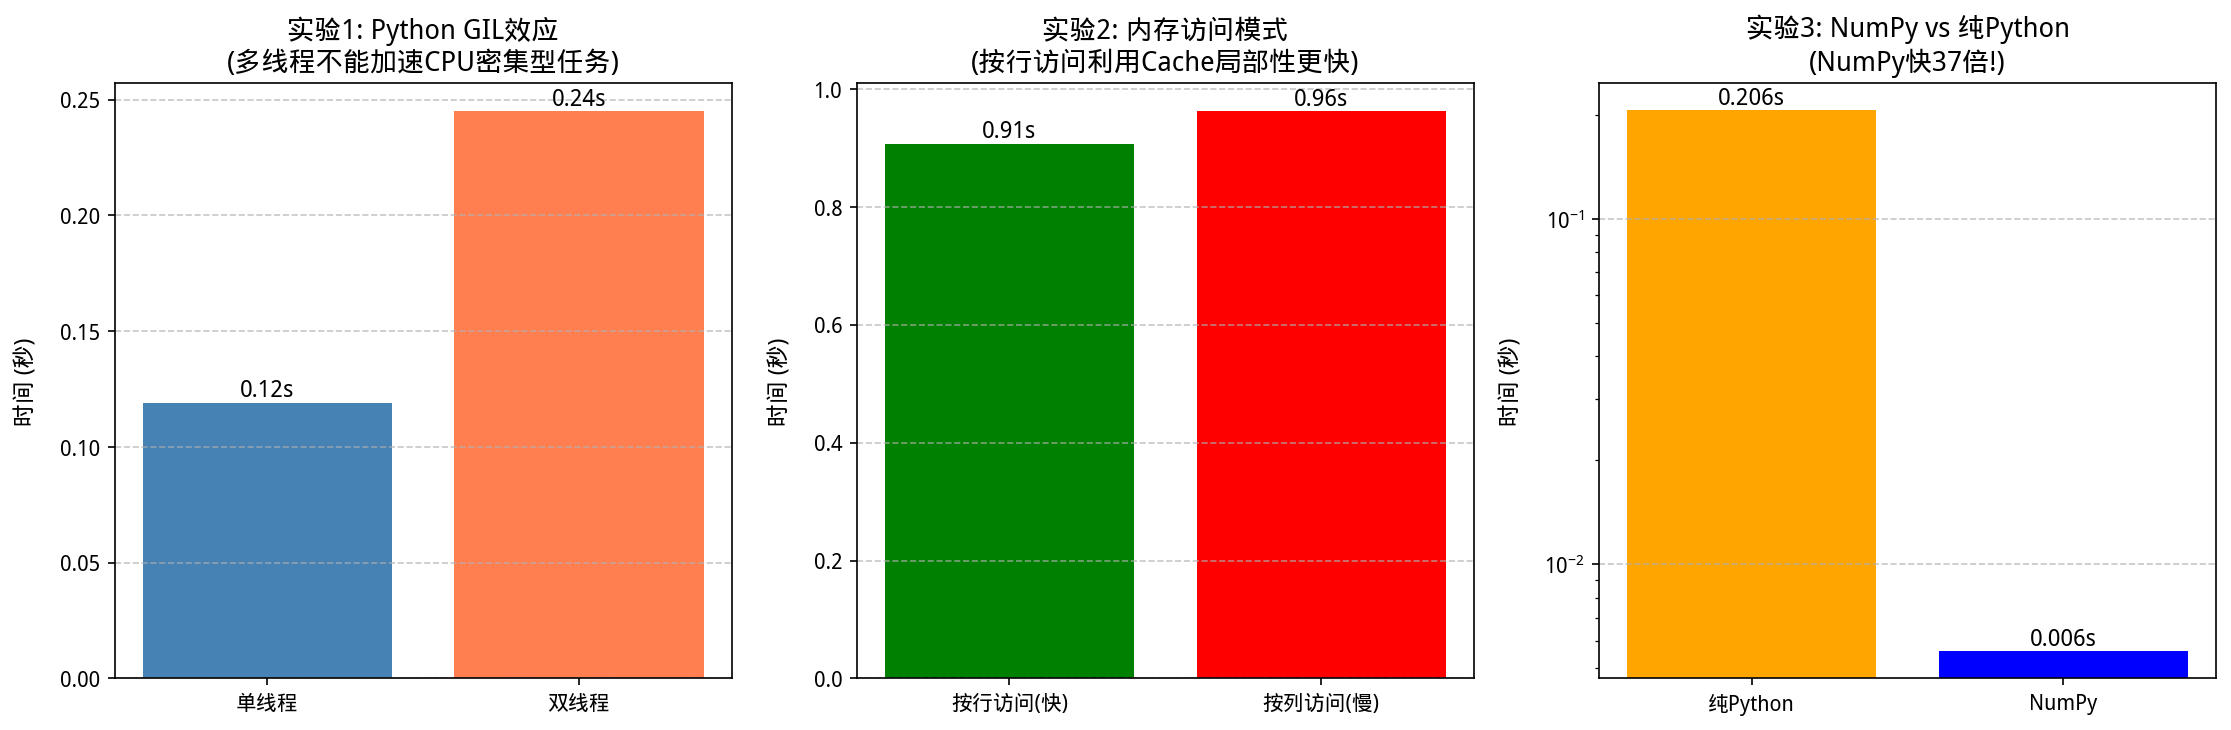
\includegraphics[width=0.95\textwidth]{figs/chap05_fig1.png}
\caption{Python性能优化实验：GIL对多线程的影响、缓存局部性的重要性、以及NumPy向量化的加速效果。左图显示Python多线程在CPU密集任务上受GIL限制，multiprocessing才能真正并行；中图展示行优先vs列优先遍历的性能差异（缓存局部性）；右图对比循环与向量化操作的速度——向量化可获得数十倍加速。}
\label{fig:chap05_python}
\end{figure}

\begin{figure}[htbp]
\centering
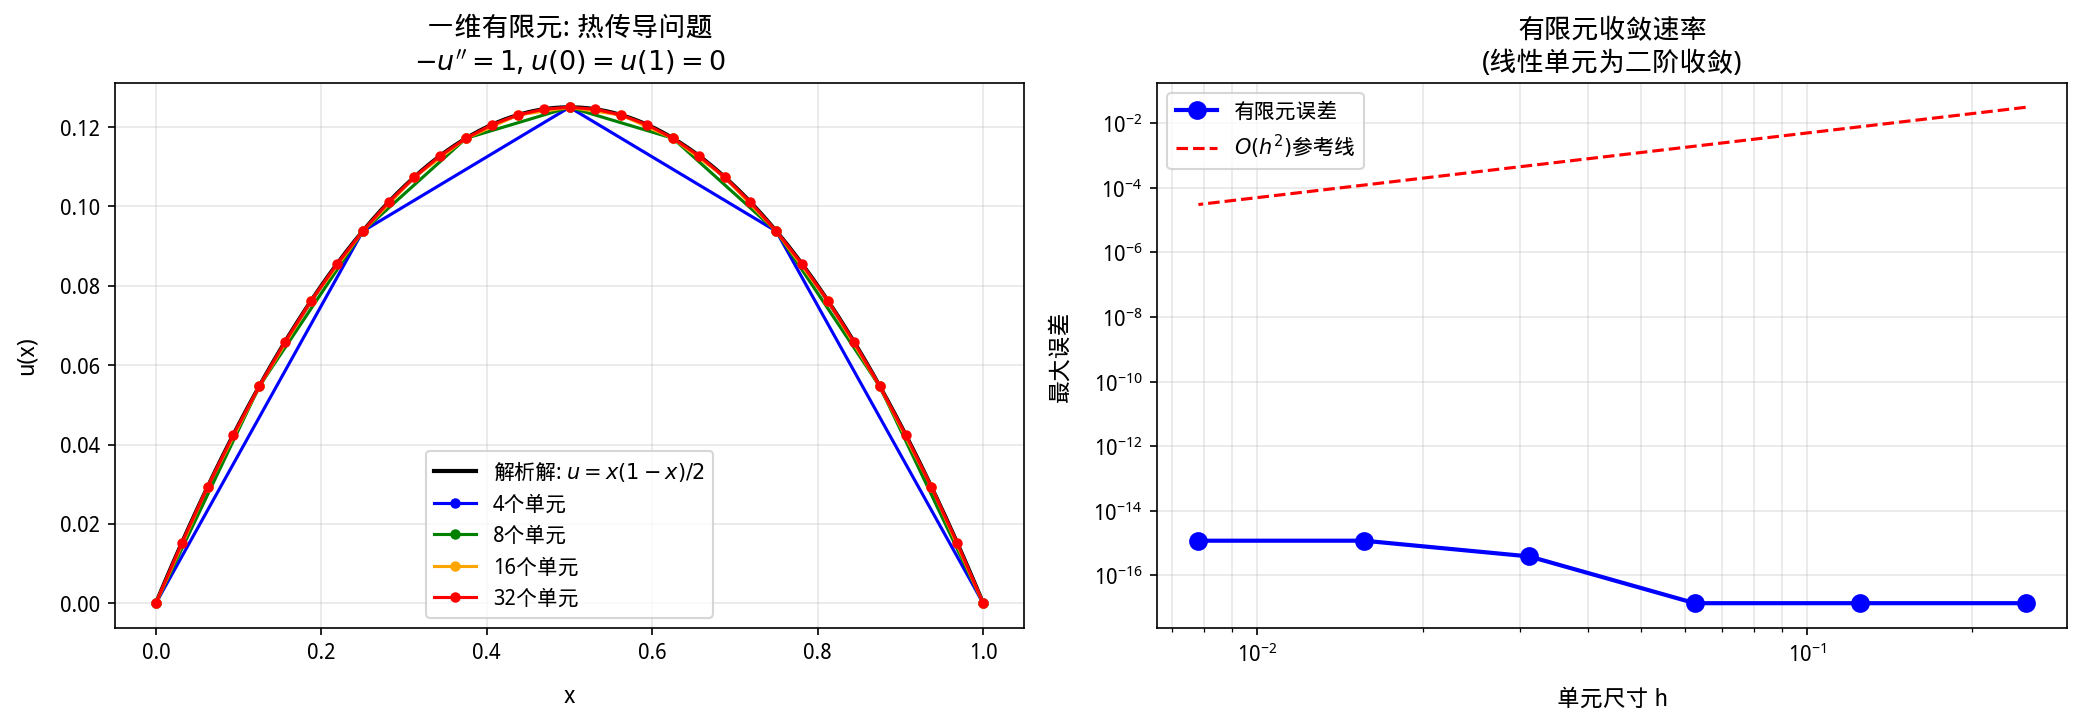
\includegraphics[width=0.95\textwidth]{figs/chap05_fig2.png}
\caption{一维有限元求解热传导问题。左图展示有限元解与解析解$u(x) = x(1-x)/2$的对比，二者几乎完全重合；中图显示刚度矩阵$K$的三对角稀疏结构——这源于帐篷函数的局部支撑性；右图展示网格细化时的收敛行为，验证了线性元的$O(h^2)$收敛阶。}
\label{fig:chap05_fem}
\end{figure}

% ------------------------------------------------------------------------------------
\section{本章小结}

\begin{enumerate}
    \item \textbf{核心思想}：有限元方法把无限维的变分问题转化为有限维的线性方程组 $KU = F$。
    
    \item \textbf{与有限差分的关系}：一维等价，二维开始分化；FEM 的优势在于处理复杂几何。
    
    \item \textbf{连续性}：$C^0$ 连续性保证能量有限；线性单元靠"两点定一线"自动满足连续性。
    
    \item \textbf{全局视角}：有限元解是全局"帐篷"基函数的线性叠加。
    
    \item \textbf{稀疏性}：基函数的局部支撑性导致刚度矩阵稀疏。
    
    \item \textbf{优化视角}：有限元 $\Leftrightarrow$ 能量最小化 $\Leftrightarrow$ 带约束的 QP 问题。
    
    \item \textbf{间断有限元}：放弃强制连续性，用约束/罚函数缝合，获得天然并行性。
\end{enumerate}

\begin{unification}[title=有限元：优化视角的大统一]
\begin{center}
\begin{tabular}{lll}
\toprule
\textbf{优化概念} & \textbf{有限元对应} & \textbf{物理意义} \\
\midrule
决策变量 & 节点值 $U_i$ & 物理量（温度/位移） \\
目标函数 & $\frac{1}{2}U^\top KU - F^\top U$ & 总势能 \\
等式约束 & Dirichlet 边界条件 & 固定边界 \\
拉格朗日乘子 & 边界反力 & 约束力 \\
罚函数 & 界面耦合项 & 虚拟弹簧 \\
\bottomrule
\end{tabular}
\end{center}

有限元不是孤立的数值技术，它是\textbf{变分原理}和\textbf{约束优化}在工程中的自然统一！

从第1章的拉格朗日乘子，到这里的有限元，$\lambda$ 始终扮演着"约束力"的角色。
\end{unification}


% ------------------------------------------------------------------------------------
\section{习题}

\paragraph{计算题}
\begin{enumerate}
    \item 用 2 个线性单元求解 $-u'' = 1$，$u(0) = u(1) = 0$。
    \begin{enumerate}
        \item 写出刚度矩阵 $K$ 和载荷向量 $F$
        \item 求解线性方程组，得到节点值 $U_1$
        \item 与精确解 $u(0.5) = 0.125$ 比较
    \end{enumerate}
    
    \item 用 4 个线性单元求解 $-u'' = \sin(\pi x)$，$u(0) = u(1) = 0$。
    \begin{enumerate}
        \item 计算载荷向量（需要积分 $\int \sin(\pi x) \phi_i dx$）
        \item 求解节点值
        \item 与精确解 $u(x) = \frac{\sin(\pi x)}{\pi^2}$ 比较
    \end{enumerate}
    
    \item 考虑非齐次边界条件：$-u'' = 0$，$u(0) = 0$，$u(1) = 1$。
    \begin{enumerate}
        \item 用 3 个单元建立有限元方程
        \item 用直接消去法处理边界条件
        \item 求解并验证结果是直线 $u(x) = x$
    \end{enumerate}
\end{enumerate}

\paragraph{证明题}
\begin{enumerate}
    \setcounter{enumi}{3}
    \item 证明刚度矩阵 $K$ 是对称的：$K_{ij} = K_{ji}$。
    
    \item 证明刚度矩阵 $K$ 是半正定的：$U^\top K U \geq 0$ 对所有 $U$ 成立。
    
    \item 证明有限元解 $u_h$ 是精确解 $u$ 在有限元空间中的"最佳逼近"：
    \[
    \int_0^1 (u_h' - u')^2 dx \leq \int_0^1 (v_h' - u')^2 dx \quad \forall v_h \in V_h
    \]
    （提示：这叫做 Galerkin 正交性）
\end{enumerate}

\paragraph{编程题}
\begin{enumerate}
    \setcounter{enumi}{6}
    \item 实现一维线性有限元：
    \begin{enumerate}
        \item 输入：区间 $[0, 1]$，单元数 $N$，源项 $f(x)$，边界值
        \item 输出：节点值向量 $U$
        \item 测试：$-u'' = 1$，$u(0) = u(1) = 0$
    \end{enumerate}
    
    \item 做收敛性实验：
    \begin{enumerate}
        \item 用 $N = 4, 8, 16, 32, 64$ 个单元求解
        \item 计算误差 $\|u - u_h\|_{L^2}$（用数值积分）
        \item 画 $\log(\text{误差})$ vs $\log(h)$ 的图，验证 $O(h^2)$ 收敛
    \end{enumerate}
    
    \item （挑战）实现二维三角形有限元：
    \begin{enumerate}
        \item 对单位正方形用三角形网格剖分
        \item 组装刚度矩阵和载荷向量
        \item 求解 $-\nabla^2 u = 1$，$u|_{\partial\Omega} = 0$
        \item 可视化数值解
    \end{enumerate}
\end{enumerate}

\paragraph{思考题}
\begin{enumerate}
    \setcounter{enumi}{9}
    \item 有限元方法和有限差分方法有什么本质区别？各有什么优缺点？
    
    \item 为什么有限元在工程中如此成功？它解决了工程师的什么痛点？
    
    \item 有限元方法与第13章的 PINN（物理信息神经网络）有什么联系和区别？
    
    \item 如果你要模拟一架飞机的应力分布，需要多少个有限元节点？这对计算机的要求是什么？
\end{enumerate}



% ====================================================================================
\section*{扩展阅读：大规模线性方程组的求解艺术}
\addcontentsline{toc}{section}{扩展阅读：大规模线性方程组的求解艺术}
% ====================================================================================

\begin{tcolorbox}[colback=gray!5, colframe=gray!50, title=本节导读]
有限元方法的最后一步是求解线性方程组 $KU = F$。这看起来很简单——不就是解个方程吗？

但当工程师模拟一架波音787的应力时，这个方程组可能有\textbf{上亿个未知数}。如何高效求解？答案涉及到一些深刻的数学概念：条件数、稀疏性、并行计算和预条件子。

更令人惊讶的是，这些概念在现代机器学习中同样重要——神经网络的训练本质上也是在求解大规模方程组！
\end{tcolorbox}

% ------------------------------------------------------------------------------------
\subsection*{一、条件数：方程组的"健康指标"}

\subsubsection*{一个令人困惑的现象}

考虑两个看起来很相似的方程组：

\begin{minipage}[t]{0.48\textwidth}
\textbf{方程组 A}
\[
\begin{pmatrix} 1 & 0 \\ 0 & 1 \end{pmatrix}
\begin{pmatrix} x \\ y \end{pmatrix}
= \begin{pmatrix} 1 \\ 1 \end{pmatrix}
\]
解：$x = 1, y = 1$

如果右边有小扰动 $(1.01, 0.99)$：

解变成 $x = 1.01, y = 0.99$

\textbf{扰动 1\%，解也变化 1\%}
\end{minipage}
\hfill
\begin{minipage}[t]{0.48\textwidth}
\textbf{方程组 B}
\[
\begin{pmatrix} 1 & 1 \\ 1 & 1.0001 \end{pmatrix}
\begin{pmatrix} x \\ y \end{pmatrix}
= \begin{pmatrix} 2 \\ 2.0001 \end{pmatrix}
\]
解：$x = 1, y = 1$

如果右边有小扰动 $(2.01, 2.0001)$：

解变成 $x = 101, y = -99$

\textbf{扰动 0.5\%，解变化 10000\%！}
\end{minipage}

\vspace{0.5cm}

为什么方程组 B 如此"敏感"？这就是\textbf{条件数}要回答的问题。

\subsubsection*{条件数的定义}

\begin{keyformula}[title=条件数]
矩阵 $A$ 的\textbf{条件数}定义为：
\begin{equation}
\kappa(A) = \|A\| \cdot \|A^{-1}\| = \frac{\sigma_{\max}(A)}{\sigma_{\min}(A)} = \frac{\text{最大奇异值}}{\text{最小奇异值}}
\end{equation}

对于对称正定矩阵（如有限元刚度矩阵）：
\begin{equation}
\kappa(K) = \frac{\lambda_{\max}(K)}{\lambda_{\min}(K)} = \frac{\text{最大特征值}}{\text{最小特征值}}
\end{equation}
\end{keyformula}

\textbf{条件数的意义}：

\begin{itemize}
    \item $\kappa \approx 1$：方程组"健康"，对扰动不敏感
    \item $\kappa \gg 1$：方程组"病态"，小扰动可能导致大误差
    \item $\kappa = \infty$：矩阵奇异，方程无唯一解
\end{itemize}

\begin{figure}[h]
\centering
\begin{tikzpicture}[scale=1.5]
    % 左边：良态矩阵
    \begin{scope}
        \node[font=\bfseries] at (1, 2.3) {良态 $\kappa \approx 1$};
        \draw[->] (0, 0) -- (2.2, 0) node[right] {$x$};
        \draw[->] (0, 0) -- (0, 2.2) node[above] {$y$};
        
        % 单位圆
        \draw[blue, thick] (1, 1) circle (0.7);
        \node[blue] at (1, 0.1) {输入扰动};
        
        % 输出也是圆（差不多大小）
        \draw[red, thick, dashed] (1, 1) ellipse (0.8 and 0.6);
        \node[red] at (1.8, 1.8) {输出误差};
    \end{scope}
    
    % 右边：病态矩阵
    \begin{scope}[xshift=4cm]
        \node[font=\bfseries] at (1, 2.3) {病态 $\kappa \gg 1$};
        \draw[->] (0, 0) -- (2.2, 0) node[right] {$x$};
        \draw[->] (0, 0) -- (0, 2.2) node[above] {$y$};
        
        % 单位圆
        \draw[blue, thick] (1, 1) circle (0.3);
        \node[blue] at (1, 0.5) {输入扰动};
        
        % 输出是扁长椭圆
        \draw[red, thick, dashed, rotate around={30:(1,1)}] (1, 1) ellipse (1.5 and 0.15);
        \node[red] at (2.2, 1.8) {输出误差};
        \node[red, font=\scriptsize] at (2.2, 1.5) {被放大！};
    \end{scope}
\end{tikzpicture}
\caption{条件数的几何意义：病态矩阵把圆形扰动拉成细长椭圆}
\end{figure}

\subsubsection*{有限元刚度矩阵的条件数}

有限元刚度矩阵的条件数与网格步长 $h$ 密切相关：

\begin{keytheorem}[title=刚度矩阵条件数估计]
对于一维 Poisson 方程的有限元刚度矩阵：
\begin{equation}
\kappa(K) \sim O\left(\frac{1}{h^2}\right)
\end{equation}

网格加密一倍（$h \to h/2$），条件数增大约 4 倍！
\end{keytheorem}

\textbf{为什么会这样？}

回顾刚度矩阵的三对角结构：
\[
K = \frac{1}{h}
\begin{pmatrix}
2 & -1 & & \\
-1 & 2 & -1 & \\
& \ddots & \ddots & \ddots \\
& & -1 & 2
\end{pmatrix}
\]

这个矩阵的特征值可以精确计算：
\begin{equation}
\lambda_k = \frac{4}{h} \sin^2\left(\frac{k\pi h}{2}\right), \quad k = 1, 2, \ldots, N-1
\end{equation}

\begin{itemize}
    \item 最小特征值：$\lambda_1 \approx \frac{4}{h} \cdot \frac{\pi^2 h^2}{4} = \pi^2 h$
    \item 最大特征值：$\lambda_{N-1} \approx \frac{4}{h}$
\end{itemize}

所以：
\[
\kappa(K) = \frac{\lambda_{\max}}{\lambda_{\min}} \approx \frac{4/h}{\pi^2 h} = \frac{4}{\pi^2 h^2} \sim O(h^{-2})
\]

\begin{physicalmeaning}
条件数与物理的关系：

\begin{itemize}
    \item \textbf{最大特征值}对应高频振动模式（相邻节点反向运动）——局部、快速
    \item \textbf{最小特征值}对应低频振动模式（整体缓慢变形）——全局、慢速
\end{itemize}

网格越细，高频和低频的差距越大，条件数越大。

这就像一根弦：基频（整体振动）和高次谐波（局部振动）的频率差距可以很大。
\end{physicalmeaning}

\subsubsection*{条件数对计算的影响}

条件数影响两件事：

\textbf{1. 直接求解的精度}

用 Gaussian 消元法求解时，舍入误差会被放大约 $\kappa$ 倍。

如果 $\kappa = 10^{10}$，双精度浮点数（约15位有效数字）只能保证约5位精度！

\textbf{2. 迭代求解的速度}

很多迭代算法（如共轭梯度法）的收敛速度与条件数直接相关：

\begin{equation}
\text{迭代次数} \sim O(\sqrt{\kappa})
\end{equation}

$\kappa = 10^6$ 意味着需要约 $1000$ 次迭代！

% ------------------------------------------------------------------------------------
\subsection*{二、稀疏矩阵：大自然的礼物}

\subsubsection*{什么是稀疏矩阵？}

\begin{definition}[稀疏矩阵]
如果一个 $n \times n$ 矩阵中非零元素的个数远小于 $n^2$（通常是 $O(n)$ 量级），我们称它为\textbf{稀疏矩阵}。
\end{definition}

有限元刚度矩阵就是典型的稀疏矩阵！

\begin{example}[波音787的有限元模型]
假设有 $n = 10^7$（一千万）个节点：

\begin{itemize}
    \item 稠密矩阵：$10^7 \times 10^7 = 10^{14}$ 个元素
        \begin{itemize}
            \item 存储：$10^{14} \times 8$ bytes $= 800$ TB（存不下！）
            \item 求解：$O(n^3) = 10^{21}$ 次运算（算不完！）
        \end{itemize}
    \item 稀疏矩阵：每行约 30 个非零元（三维问题）
        \begin{itemize}
            \item 存储：$3 \times 10^8$ 个非零元 $\approx 2.4$ GB（轻松！）
            \item 求解：使用稀疏求解器，可行！
        \end{itemize}
\end{itemize}
\end{example}

\subsubsection*{三对角矩阵：最简单的稀疏结构}

一维有限元产生的三对角矩阵是最简单的稀疏矩阵：

\[
K = \begin{pmatrix}
a_1 & c_1 & & & \\
b_2 & a_2 & c_2 & & \\
& b_3 & a_3 & c_3 & \\
& & \ddots & \ddots & \ddots \\
& & & b_n & a_n
\end{pmatrix}
\]

\textbf{Thomas 算法}（追赶法）可以在 $O(n)$ 时间内求解！

\noindent\textbf{算法：Thomas 算法（三对角系统求解）}

\medskip
\noindent\textbf{步骤：}

\begin{enumerate}
  \item \textbf{前向消元（从上到下）}
  \begin{enumerate}
      \item 对 $i=2,\dots,n$：
      \begin{itemize}
          \item $w = b_i / a_{i-1}$\hfill{\footnotesize（使第 $i$ 行以第 $i\!-\!1$ 行为基准做消元）}
          \item $a_i \leftarrow a_i - w \cdot c_{i-1}$\hfill{\footnotesize（更新主对角：消掉 $b_i$）}
          \item $f_i \leftarrow f_i - w \cdot f_{i-1}$\hfill{\footnotesize（右端项同样做线性消元）}
      \end{itemize}
  \end{enumerate}

  \item \textbf{回代（从下到上）}
  \begin{enumerate}
      \item 计算：$x_n = f_n / a_n$\hfill{\footnotesize（链条最末端最简单，从这里开始回传信息）}
      \item 对 $i = n-1, n-2, \dots, 1$：
      \begin{itemize}
          \item $x_i = (f_i - c_i \cdot x_{i+1}) / a_i$\hfill{\footnotesize（依次向上回代解）}
      \end{itemize}
  \end{enumerate}
\end{enumerate}

\begin{insightbox}
\textbf{Thomas 算法的本质}：

三对角系统就像一条链：
\[
\bullet - \bullet - \bullet - \bullet - \bullet
\]

每个节点只与相邻节点耦合。

前向消元将链条“一节节剪断”，回代将解“一节节传回”。

本质上就是一种线性结构的动态规划。
\end{insightbox}


\subsubsection*{带状矩阵与块三对角矩阵}

二维和三维问题的刚度矩阵虽然不是三对角，但仍有规律的稀疏结构：

\begin{figure}[h]
\centering
\begin{tikzpicture}[scale=0.55]

    % -------------------------------
    % 一维：三对角
    % -------------------------------
    \begin{scope}[xshift=0cm]
        \node[font=\bfseries] at (2.5, 6) {一维：三对角};
        \draw[gray] (0,0) rectangle (5,5);

        % 主对角
        \foreach \i in {0,...,4} {
            \fill[blue!60] (\i, 4-\i) rectangle ++(1,1);
        }
        % 上下对角
        \foreach \i in {0,...,3} {
            \fill[blue!30] (\i+1, 4-\i) rectangle ++(1,1);
            \fill[blue!30] (\i, 3-\i) rectangle ++(1,1);
        }

        \node at (2.5, -0.8) {\small 带宽 = 1};
    \end{scope}


    % -------------------------------
    % 二维：带状
    % -------------------------------
    \begin{scope}[xshift=8.5cm]
        \node[font=\bfseries] at (3, 6) {二维：带状};
        \draw[gray] (0,0) rectangle (6,6);

        % 主对角
        \foreach \i in {0,...,5} {
            \fill[blue!60] (\i, 5-\i) rectangle ++(1,1);
        }
        % 近对角
        \foreach \i in {0,...,4} {
            \fill[blue!30] (\i+1, 5-\i) rectangle ++(1,1);
            \fill[blue!30] (\i, 4-\i) rectangle ++(1,1);
        }
        % 远对角（来自另一方向）
        \foreach \i in {0,...,2} {
            \fill[blue!15] (\i+3, 5-\i) rectangle ++(1,1);
            \fill[blue!15] (\i, 2-\i) rectangle ++(1,1);
        }

        \node at (3, -0.8) {\small 带宽 $\approx \sqrt{n}$};
    \end{scope}


    % -------------------------------
    % 三维：更宽的带
    % -------------------------------
    \begin{scope}[xshift=17cm]
        \node[font=\bfseries] at (3.5, 6) {三维：更宽的带};
        \draw[gray] (0,0) rectangle (7,7);

        % 主对角
        \foreach \i in {0,...,6} {
            \fill[blue!60] (\i, 6-\i) rectangle ++(1,1);
        }

        % 逐步扩散的带状
        \foreach \d in {1,2,3} {
            \pgfmathsetmacro{\alpha}{60-15*\d}
            \foreach \i in {0,...,\numexpr6-\d} {
                \fill[blue!\alpha] (\i+\d, 6-\i) rectangle ++(1,1);
                \fill[blue!\alpha] (\i, 6-\i-\d) rectangle ++(1,1);
            }
        }

        \node at (3.5, -0.8) {\small 带宽 $\approx n^{2/3}$};
    \end{scope}

\end{tikzpicture}
\caption{不同维度问题的刚度矩阵稀疏结构}
\end{figure}


\textbf{带宽}决定了直接求解所需的计算量：

\begin{center}
\begin{tabular}{c|c|c|c}
\toprule
问题维度 & 带宽 $b$ & 求解复杂度 & $n = 10^6$ 时 \\
\midrule
一维 & $O(1)$ & $O(n)$ & $10^6$ 次运算 \\
二维 & $O(\sqrt{n})$ & $O(n \cdot b^2) = O(n^2)$ & $10^{12}$ 次运算 \\
三维 & $O(n^{2/3})$ & $O(n \cdot b^2) = O(n^{7/3})$ & $10^{14}$ 次运算 \\
\bottomrule
\end{tabular}
\end{center}

这就是为什么\textbf{大规模三维问题必须用迭代法}。

% ------------------------------------------------------------------------------------
\subsection*{三、并行计算：分而治之}

\subsubsection*{为什么三对角求解难以并行？}

Thomas 算法虽然快（$O(n)$），但它是\textbf{串行}的：

\begin{itemize}
    \item 前向消元：第 $i$ 步依赖第 $i-1$ 步的结果
    \item 回代：第 $i$ 步依赖第 $i+1$ 步的结果
\end{itemize}

就像多米诺骨牌，必须一个接一个倒下，不能跳跃！

\begin{figure}[h]
\centering
\begin{tikzpicture}[scale=0.8]
    % 串行
    \node[font=\bfseries] at (3, 2) {串行 Thomas 算法};
    \foreach \i in {1,...,6} {
        \draw[thick, fill=blue!30] (\i, 0) rectangle ++(0.6, 1);
        \node at (\i+0.3, 0.5) {\small $\i$};
    }
    \draw[->, thick, red] (1.3, 0.5) -- (1.7, 0.5);
    \draw[->, thick, red] (2.3, 0.5) -- (2.7, 0.5);
    \draw[->, thick, red] (3.3, 0.5) -- (3.7, 0.5);
    \draw[->, thick, red] (4.3, 0.5) -- (4.7, 0.5);
    \draw[->, thick, red] (5.3, 0.5) -- (5.7, 0.5);
    \node at (3.5, -0.8) {\small 必须按顺序执行};
\end{tikzpicture}
\end{figure}

\subsubsection*{域分解：把问题切开}

一个聪明的想法：把计算域\textbf{分成几块}，每块独立求解，然后把边界"缝合"起来。

\begin{figure}[h]
\centering
\begin{tikzpicture}[scale=1.2]
    % 原始问题
    \begin{scope}
        \node[font=\bfseries] at (2, 1.5) {原始问题};
        \draw[thick] (0, 0) -- (4, 0);
        \foreach \i in {0,...,8} {
            \fill (\i*0.5, 0) circle (2pt);
        }
        \node at (2, -0.5) {8个节点，一个方程组};
    \end{scope}
    
    % 箭头
    \draw[->, very thick] (4.5, 0) -- (5.5, 0);
    
    % 分解后
    \begin{scope}[xshift=6cm]
        \node[font=\bfseries] at (2, 1.5) {域分解};
        
        % 子域1
        \draw[thick, blue] (0, 0) -- (1.8, 0);
        \foreach \i in {0,...,3} {
            \fill[blue] (\i*0.5, 0) circle (2pt);
        }
        \node[blue] at (0.9, 0.4) {子域1};
        
        % 子域2
        \draw[thick, red] (2.2, 0) -- (4, 0);
        \foreach \i in {5,...,8} {
            \fill[red] (\i*0.5, 0) circle (2pt);
        }
        \node[red] at (3.1, 0.4) {子域2};
        
        % 界面
        \draw[thick, green!60!black, dashed] (1.8, -0.3) -- (2.2, -0.3);
        \fill[green!60!black] (2, 0) circle (3pt);
        \node[green!60!black] at (2, -0.7) {界面};
        
        \node at (2, -1.2) {两个小方程组 + 界面条件};
    \end{scope}
\end{tikzpicture}
\caption{域分解的基本思想}
\end{figure}

\subsubsection*{Schur 补：界面上的方程}

设原方程组为：
\[
\begin{pmatrix}
A_{11} & A_{12} & 0 \\
A_{21} & A_{22} & A_{23} \\
0 & A_{32} & A_{33}
\end{pmatrix}
\begin{pmatrix}
u_1 \\ u_\Gamma \\ u_2
\end{pmatrix}
=
\begin{pmatrix}
f_1 \\ f_\Gamma \\ f_2
\end{pmatrix}
\]

其中 $u_1, u_2$ 是两个子域的内部节点，$u_\Gamma$ 是界面节点。

从第一个和第三个方程解出 $u_1, u_2$（关于 $u_\Gamma$ 的函数），代入第二个方程：

\begin{equation}
\underbrace{\left(A_{22} - A_{21}A_{11}^{-1}A_{12} - A_{23}A_{33}^{-1}A_{32}\right)}_{S: \text{Schur 补}} u_\Gamma = \tilde{f}_\Gamma
\end{equation}


\paragraph{推导 Schur 补}

把矩阵方程展开成三个方程：
\begin{align}
A_{11} u_1 + A_{12} u_\Gamma &= f_1 \tag{子域1内部} \\
A_{21} u_1 + A_{22} u_\Gamma + A_{23} u_2 &= f_\Gamma \tag{界面} \\
A_{32} u_\Gamma + A_{33} u_2 &= f_2 \tag{子域2内部}
\end{align}

\textbf{第一步}：从方程(1)解出 $u_1$（把 $u_\Gamma$ 当作已知量）
\[
u_1 = A_{11}^{-1}(f_1 - A_{12} u_\Gamma)
\]

\textbf{第二步}：从方程(3)解出 $u_2$（把 $u_\Gamma$ 当作已知量）
\[
u_2 = A_{33}^{-1}(f_2 - A_{32} u_\Gamma)
\]

\textbf{第三步}：把 $u_1, u_2$ 代入方程(2)，消去内部自由度
\begin{align*}
A_{21} \cdot \underbrace{A_{11}^{-1}(f_1 - A_{12} u_\Gamma)}_{u_1} + A_{22} u_\Gamma + A_{23} \cdot \underbrace{A_{33}^{-1}(f_2 - A_{32} u_\Gamma)}_{u_2} &= f_\Gamma
\end{align*}

展开并整理（把 $u_\Gamma$ 的项放到左边，常数项放到右边）：
\[
\underbrace{\left(A_{22} - A_{21}A_{11}^{-1}A_{12} - A_{23}A_{33}^{-1}A_{32}\right)}_{S:\text{ Schur 补}} u_\Gamma = \underbrace{f_\Gamma - A_{21}A_{11}^{-1}f_1 - A_{23}A_{33}^{-1}f_2}_{\tilde{f}_\Gamma:\text{ 修正后的右端项}}
\]


\begin{keyformula}[title=Schur 补方法]
\begin{enumerate}
    \item \textbf{并行}：在每个子域上独立计算 $A_{11}^{-1}$ 和 $A_{33}^{-1}$
    \item \textbf{组装}：形成界面上的 Schur 补系统 $S u_\Gamma = \tilde{f}_\Gamma$
    \item \textbf{求解}：解这个小得多的界面方程
    \item \textbf{并行}：用 $u_\Gamma$ 回代得到各子域的解
\end{enumerate}
\end{keyformula}

\begin{physicalmeaning}
Schur 补的物理意义：

想象把一根弹簧链在中间切断，两边分别"凝缩"成等效刚度。

$S$ 就是界面上的\textbf{等效刚度}——它告诉你：如果界面位移是 $u_\Gamma$，界面上受到的力是多少。

这与第1章中消去部分变量得到约束力的想法完全一致！
\end{physicalmeaning}


\begin{insightbox}
\textbf{并行计算的智慧}：

串行算法追求的是\textbf{减少总工作量}。

并行算法追求的是\textbf{减少依赖深度}——即使总工作量增加，只要能并行就值得！

Schur补的总运算量比 Thomas 算法多，但它的\textbf{并行深度}是 $O(\log n)$，这使得在 GPU 上可以获得巨大加速。
\end{insightbox}

% ------------------------------------------------------------------------------------
\subsection*{四、预条件子：让迭代飞起来}

\subsubsection*{迭代法的基本思想}

当问题太大，直接求解不现实时，我们转向\textbf{迭代法}：

从一个初始猜测 $U^{(0)}$ 开始，逐步改进：
\[
U^{(0)} \to U^{(1)} \to U^{(2)} \to \cdots \to U^*
\]

\paragraph{最简单的迭代法：Jacobi 迭代}

考虑线性方程组 $KU = F$，写成分量形式：
\[
\sum_{j=1}^{n} K_{ij} U_j = F_i, \quad i = 1, 2, \ldots, n
\]

把第 $i$ 个方程中的 $U_i$ 单独拿出来：
\[
K_{ii} U_i + \sum_{j \neq i} K_{ij} U_j = F_i
\]

解出 $U_i$：
\[
U_i = \frac{1}{K_{ii}} \left( F_i - \sum_{j \neq i} K_{ij} U_j \right)
\]

\textbf{Jacobi 迭代}的想法：用旧的 $U^{(k)}$ 计算右边，得到新的 $U^{(k+1)}$：

\begin{tcolorbox}[colback=gray!5, colframe=gray!60, title=Jacobi 迭代]
\begin{equation}
U_i^{(k+1)} = \frac{1}{K_{ii}} \left( F_i - \sum_{j \neq i} K_{ij} U_j^{(k)} \right), \quad i = 1, 2, \ldots, n
\end{equation}

或者用矩阵形式：
\[
U^{(k+1)} = D^{-1}(F - (K-D)U^{(k)})
\]
其中 $D = \text{diag}(K)$ 是 $K$ 的对角部分。
\end{tcolorbox}

\paragraph{一个具体例子}

求解：
\[
\begin{pmatrix} 4 & 1 \\ 1 & 3 \end{pmatrix} \begin{pmatrix} U_1 \\ U_2 \end{pmatrix} = \begin{pmatrix} 1 \\ 2 \end{pmatrix}
\]

精确解是 $U_1 = 1/11 \approx 0.091$，$U_2 = 7/11 \approx 0.636$。

\textbf{Jacobi 迭代公式}：
\begin{align}
U_1^{(k+1)} &= \frac{1}{4}\left(1 - 1 \cdot U_2^{(k)}\right) = \frac{1 - U_2^{(k)}}{4} \\
U_2^{(k+1)} &= \frac{1}{3}\left(2 - 1 \cdot U_1^{(k)}\right) = \frac{2 - U_1^{(k)}}{3}
\end{align}

从 $U^{(0)} = (0, 0)$ 开始迭代：

\begin{center}
\begin{tabular}{c|c|c|c}
\toprule
迭代次数 $k$ & $U_1^{(k)}$ & $U_2^{(k)}$ & 误差 $\|U^{(k)} - U^*\|$ \\
\midrule
0 & 0 & 0 & 0.643 \\
1 & 0.250 & 0.667 & 0.162 \\
2 & 0.083 & 0.583 & 0.053 \\
3 & 0.104 & 0.639 & 0.013 \\
4 & 0.090 & 0.632 & 0.004 \\
5 & 0.092 & 0.637 & 0.001 \\
$\vdots$ & $\vdots$ & $\vdots$ & $\vdots$ \\
$\infty$ & 0.091 & 0.636 & 0 \\
\bottomrule
\end{tabular}
\end{center}

\begin{figure}[h]
\centering
\begin{tikzpicture}[scale=4]
    % 坐标轴
    \draw[->] (-0.1, 0) -- (0.35, 0) node[right] {$U_1$};
    \draw[->] (0, -0.1) -- (0, 0.8) node[above] {$U_2$};
    
    % 精确解
    \fill[red] (0.091, 0.636) circle (1pt);
    \node[red, above right] at (0.091, 0.636) {\small 精确解};
    
    % 迭代轨迹
    \draw[blue, thick, ->] (0, 0) -- (0.25, 0.667);
    \draw[blue, thick, ->] (0.25, 0.667) -- (0.083, 0.583);
    \draw[blue, thick, ->] (0.083, 0.583) -- (0.104, 0.639);
    \draw[blue, thick, ->] (0.104, 0.639) -- (0.090, 0.632);
    \draw[blue, thick, ->] (0.090, 0.632) -- (0.092, 0.637);
    
    % 起点
    \fill[blue] (0, 0) circle (1pt);
    \node[blue, below left] at (0, 0) {\small 起点};
\end{tikzpicture}
\caption{Jacobi 迭代的轨迹：螺旋式逼近精确解}
\end{figure}

\paragraph{Jacobi 迭代的物理直觉}

对于有限元方程，Jacobi 迭代有很好的物理解释：

\begin{physicalmeaning}
想象一个弹簧网络处于非平衡状态。

Jacobi 迭代的每一步：
\begin{enumerate}
    \item 看每个节点受到的"不平衡力"：$r_i = F_i - \sum_j K_{ij} U_j$（残差）
    \item 假设其他节点不动，只调整当前节点来平衡这个力
    \item 同时对所有节点做这个调整
\end{enumerate}

就像同时轻轻推动所有不平衡的节点，让系统逐渐趋于平衡。
\end{physicalmeaning}

\paragraph{Jacobi vs Gauss-Seidel}

Jacobi 迭代的一个"浪费"：计算 $U_i^{(k+1)}$ 时，我们已经算出了 $U_1^{(k+1)}, \ldots, U_{i-1}^{(k+1)}$，为什么不用最新的值？

\textbf{Gauss-Seidel 迭代}就是这个改进：
\[
U_i^{(k+1)} = \frac{1}{K_{ii}} \left( F_i - \sum_{j < i} K_{ij} U_j^{(k+1)} - \sum_{j > i} K_{ij} U_j^{(k)} \right)
\]

\begin{center}
\begin{tabular}{l|c|c}
\toprule
& \textbf{Jacobi} & \textbf{Gauss-Seidel} \\
\midrule
更新方式 & 同时更新所有分量 & 依次更新每个分量 \\
使用的值 & 全用旧值 $U^{(k)}$ & 用最新可用的值 \\
收敛速度 & 较慢 & 通常快一倍 \\
并行性 & \textbf{完美并行}（各分量独立） & 串行（有依赖） \\
\bottomrule
\end{tabular}
\end{center}

\begin{insightbox}
\textbf{Jacobi 在 GPU 时代的复兴}：

Gauss-Seidel 收敛更快，但它是串行的——计算 $U_i$ 必须等 $U_1, \ldots, U_{i-1}$ 算完。

Jacobi 虽然慢，但每个分量可以\textbf{独立计算}——完美适合 GPU 的数千个核心！

在现代并行硬件上，做 2 次 Jacobi 迭代可能比做 1 次 Gauss-Seidel 还快。
\end{insightbox}

\paragraph{Jacobi 迭代的收敛性}

Jacobi 迭代不总是收敛！收敛的条件与矩阵的性质有关。

\begin{keytheorem}[title=Jacobi 收敛的充分条件]
如果矩阵 $K$ 是\textbf{严格对角占优}的：
\[
|K_{ii}| > \sum_{j \neq i} |K_{ij}|, \quad \forall i
\]
即每行的对角元绝对值大于该行其他元素绝对值之和，则 Jacobi 迭代收敛。
\end{keytheorem}

好消息：有限元刚度矩阵通常满足这个条件（或接近满足），所以 Jacobi 迭代对有限元问题通常收敛。

\vspace{0.5cm}
现在我们可以介绍更高级的迭代法了：

最重要的迭代法之一是\textbf{共轭梯度法}（CG），它把求解 $KU = F$ 转化为最小化：
\[
\min_U \quad \frac{1}{2}U^\top K U - F^\top U
\]

\paragraph{从最速下降到共轭梯度}

最直接的想法是\textbf{最速下降法}：每一步沿着负梯度方向走。

目标函数 $J(U) = \frac{1}{2}U^\top K U - F^\top U$ 的梯度是：
\[
\nabla J = KU - F = -r
\]
其中 $r = F - KU$ 叫做\textbf{残差}（residual），它衡量当前解离真实解有多远。

\begin{figure}[h]
\centering
\begin{tikzpicture}[scale=1.0]
    % 最速下降
    \begin{scope}
        \node[font=\bfseries] at (2, 3.5) {最速下降法};
        \draw[->] (0, 0) -- (4, 0) node[right] {$U_1$};
        \draw[->] (0, 0) -- (0, 3) node[above] {$U_2$};
        % 椭圆等高线
        \draw[blue!30, rotate around={0:(2,1.5)}] (2, 1.5) ellipse (1.5 and 0.5);
        \draw[blue!50, rotate around={0:(2,1.5)}] (2, 1.5) ellipse (1.0 and 0.33);
        \draw[blue!70, rotate around={0:(2,1.5)}] (2, 1.5) ellipse (0.5 and 0.17);
        \fill[red] (2, 1.5) circle (2pt);
        % 锯齿路径
        \draw[->, thick, red] (0.8, 2.2) -- (1.5, 1.1);
        \draw[->, thick, red] (1.5, 1.1) -- (1.8, 1.8);
        \draw[->, thick, red] (1.8, 1.8) -- (1.95, 1.35);
        \draw[->, thick, red] (1.95, 1.35) -- (2.0, 1.55);
        \node at (2, -0.5) {\small 锯齿形，收敛慢};
    \end{scope}
    
    % 共轭梯度
    \begin{scope}[xshift=6cm]
        \node[font=\bfseries] at (2, 3.5) {共轭梯度法};
        \draw[->] (0, 0) -- (4, 0) node[right] {$U_1$};
        \draw[->] (0, 0) -- (0, 3) node[above] {$U_2$};
        % 椭圆等高线
        \draw[blue!30, rotate around={0:(2,1.5)}] (2, 1.5) ellipse (1.5 and 0.5);
        \draw[blue!50, rotate around={0:(2,1.5)}] (2, 1.5) ellipse (1.0 and 0.33);
        \draw[blue!70, rotate around={0:(2,1.5)}] (2, 1.5) ellipse (0.5 and 0.17);
        \fill[red] (2, 1.5) circle (2pt);
        % 直接路径
        \draw[->, thick, green!60!black] (0.8, 2.2) -- (1.5, 0.9);
        \draw[->, thick, green!60!black] (1.5, 0.9) -- (2, 1.5);
        \node at (2, -0.5) {\small 最多$n$步收敛！};
    \end{scope}
\end{tikzpicture}
\caption{最速下降法会"锯齿"前进，共轭梯度法选择更聪明的方向}
\end{figure}

最速下降法的问题：在窄长的"山谷"中会来回震荡，收敛很慢。

\paragraph{共轭方向的魔力}

共轭梯度法的核心思想：不要每次都沿梯度走，而是选择\textbf{互相"共轭"的方向}。

\begin{definition}[共轭方向]
两个向量 $p$ 和 $q$ 关于矩阵 $K$ \textbf{共轭}（或 $K$-正交），如果：
\[
p^\top K q = 0
\]
\end{definition}

为什么共轭方向好？如果我们有 $n$ 个互相共轭的方向 $p_1, p_2, \ldots, p_n$，那么：

\begin{itemize}
    \item 沿 $p_1$ 走到最优 $\Rightarrow$ 这个方向上的分量"搞定了"
    \item 再沿 $p_2$ 走到最优 $\Rightarrow$ \textbf{不会破坏} $p_1$ 方向上的最优性！
    \item 最多 $n$ 步，所有方向都搞定，到达全局最优
\end{itemize}

\begin{insightbox}
\textbf{共轭 vs 正交}：

普通正交：$p^\top q = 0$（在欧几里得内积下垂直）

$K$-共轭：$p^\top K q = 0$（在 $K$ 定义的内积下垂直）

对于对称正定矩阵 $K$，可以定义内积 $\langle p, q \rangle_K = p^\top K q$。

共轭方向就是在这个"变形"的内积下互相垂直的方向！
\end{insightbox}


\begin{tcolorbox}[colback=gray!5, colframe=gray!60, title=共轭梯度法（CG）]
\textbf{输入}：对称正定矩阵 $K$，右端向量 $F$，初始猜测 $U^{(0)}$

\textbf{初始化}：
\begin{align*}
r^{(0)} &= F - K U^{(0)} & \textcolor{gray}{\text{// 初始残差}} \\
p^{(0)} &= r^{(0)} & \textcolor{gray}{\text{// 初始搜索方向 = 负梯度方向}}
\end{align*}

\textbf{迭代}：对 $k = 0, 1, 2, \ldots$

\begin{enumerate}
    \item \textbf{计算步长}（沿 $p^{(k)}$ 走多远？）
    \[
    \alpha_k = \frac{(r^{(k)})^\top r^{(k)}}{(p^{(k)})^\top K p^{(k)}} \quad \textcolor{gray}{\text{// 使 $J(U^{(k)} + \alpha p^{(k)})$ 最小的 $\alpha$}}
    \]
    
    \item \textbf{更新解}
    \[
    U^{(k+1)} = U^{(k)} + \alpha_k p^{(k)} \quad \textcolor{gray}{\text{// 沿搜索方向前进}}
    \]
    
    \item \textbf{更新残差}
    \[
    r^{(k+1)} = r^{(k)} - \alpha_k K p^{(k)} \quad \textcolor{gray}{\text{// 不用重新算 $F - KU$，省一次矩阵乘法}}
    \]
    
    \item \textbf{检查收敛}：如果 $\|r^{(k+1)}\| < \epsilon$，停止
    
    \item \textbf{计算新方向}（关键：保证与之前所有方向共轭！）
    \[
    \beta_k = \frac{(r^{(k+1)})^\top r^{(k+1)}}{(r^{(k)})^\top r^{(k)}} \quad \textcolor{gray}{\text{// Gram-Schmidt 正交化的系数}}
    \]
    \[
    p^{(k+1)} = r^{(k+1)} + \beta_k p^{(k)} \quad \textcolor{gray}{\text{// 新方向 = 残差 + 旧方向的修正}}
    \]
\end{enumerate}
\end{tcolorbox}

\paragraph{为什么这个算法如此高效？}

\begin{enumerate}
    \item \textbf{每步只需一次矩阵-向量乘法}：计算 $Kp^{(k)}$，这是主要开销
    
    \item \textbf{短递归}：$p^{(k+1)}$ 只依赖于 $p^{(k)}$ 和 $r^{(k+1)}$，不需要存储所有历史方向
    
    \item \textbf{自动共轭}：通过巧妙的 $\beta_k$ 选择，新方向自动与所有旧方向共轭（这是 CG 的数学奇迹！）
    
    \item \textbf{理论上 $n$ 步精确收敛}：对于 $n \times n$ 的矩阵，最多 $n$ 步得到精确解
\end{enumerate}

\begin{physicalmeaning}
CG 的几何直觉：

想象你在一个椭球形的山谷里找最低点。

\begin{itemize}
    \item \textbf{最速下降}：每次沿最陡的方向走，但山谷是歪的，你会来回反弹
    \item \textbf{共轭梯度}：第一步沿最陡方向，之后每步都选一个"新维度"，保证不走回头路
\end{itemize}

就像在 $n$ 维空间里，你有 $n$ 个互相垂直的方向。每走一步就"锁定"一个维度，$n$ 步后所有维度都锁定，到达最低点！
\end{physicalmeaning}

\paragraph{一个简单例子}

求解 $KU = F$，其中：
\[
K = \begin{pmatrix} 4 & 1 \\ 1 & 3 \end{pmatrix}, \quad F = \begin{pmatrix} 1 \\ 2 \end{pmatrix}, \quad U^{(0)} = \begin{pmatrix} 0 \\ 0 \end{pmatrix}
\]

\textbf{初始化}：$r^{(0)} = F - KU^{(0)} = (1, 2)^\top$，$p^{(0)} = (1, 2)^\top$

\textbf{第一步}：
\begin{align*}
Kp^{(0)} &= \begin{pmatrix} 4 & 1 \\ 1 & 3 \end{pmatrix} \begin{pmatrix} 1 \\ 2 \end{pmatrix} = \begin{pmatrix} 6 \\ 7 \end{pmatrix} \\
\alpha_0 &= \frac{1^2 + 2^2}{1 \cdot 6 + 2 \cdot 7} = \frac{5}{20} = 0.25 \\
U^{(1)} &= (0, 0)^\top + 0.25 \cdot (1, 2)^\top = (0.25, 0.5)^\top \\
r^{(1)} &= (1, 2)^\top - 0.25 \cdot (6, 7)^\top = (-0.5, 0.25)^\top
\end{align*}

\textbf{第二步}：
\begin{align*}
\beta_0 &= \frac{(-0.5)^2 + 0.25^2}{1^2 + 2^2} = \frac{0.3125}{5} = 0.0625 \\
p^{(1)} &= (-0.5, 0.25)^\top + 0.0625 \cdot (1, 2)^\top = (-0.4375, 0.375)^\top
\end{align*}

继续迭代...对于 $2 \times 2$ 的问题，\textbf{最多2步}就能得到精确解！

\subsubsection*{共轭梯度法的收敛速度}

\begin{keytheorem}[title=CG 收敛速度]
共轭梯度法的误差满足：
\begin{equation}
\|U^{(k)} - U^*\|_K \leq 2 \left(\frac{\sqrt{\kappa} - 1}{\sqrt{\kappa} + 1}\right)^k \|U^{(0)} - U^*\|_K
\end{equation}

要使误差减少到 $\epsilon$，需要迭代次数：
\begin{equation}
k \sim O\left(\sqrt{\kappa} \log(1/\epsilon)\right)
\end{equation}
\end{keytheorem}

对于有限元问题，$\kappa \sim h^{-2}$，所以 $k \sim O(h^{-1}) = O(\sqrt{n})$。

$n = 10^6$ 时需要约 $1000$ 次迭代——太慢了！

\begin{insightbox}
\textbf{条件数的几何直觉：为什么扁椭圆让迭代法痛苦？}

想象你在一个山谷中寻找最低点。迭代法就像蒙着眼睛下山——每一步只能沿着当前位置最陡的方向走。

\textbf{情况1：圆形山谷}（条件数 $\kappa \approx 1$）
\begin{itemize}
    \item 等高线是同心圆
    \item 最陡方向始终指向谷底
    \item 一步到位！
\end{itemize}

\textbf{情况2：狭长山谷}（条件数 $\kappa \gg 1$）
\begin{itemize}
    \item 等高线是扁椭圆
    \item 最陡方向指向椭圆短轴，而非谷底
    \item 结果：来回zigzag，浪费大量迭代！
\end{itemize}

\textbf{预条件子的作用}：把扁椭圆"拉圆"！

数学上，如果原问题的海森矩阵是 $A$，预条件后变成 $M^{-1}A$。好的 $M$ 能让 $M^{-1}A$ 的特征值更集中，等高线更接近圆形。
\end{insightbox}

\subsubsection*{预条件：变换问题}

\textbf{预条件}的基本思想：  
不直接求解 $KU = F$，而是先将它“变换”成一个更容易求解的线性系统。

做法是选一个矩阵 $M$（称为\textbf{预条件子}），使得新系统
\[
(M^{-1}K)U = M^{-1}F
\]
的\textbf{条件数比原系统小}，从而使迭代法收敛更快。

\textbf{好的预条件子应满足：}

\begin{itemize}
    \item $M^{-1}K$ 的条件数要小（这样迭代法收敛快）
    \item $M^{-1}v$ 要容易计算（每步迭代的代价低）
\end{itemize}

这两个要求本质上是矛盾的：

- 如果让 $M$ 与 $K$ 非常接近，那么 $M^{-1}K$ 的条件数就会非常理想（甚至当 $M = K$ 时条件数为 1）

- 但这时计算 $M^{-1}$ 本身就和解原问题一样困难，因此完全没有意义

因此，一个实用的预条件子必须在“逼近 $K$”（改善条件数）和“计算容易”（代价低）之间取得折中。

\subsubsection*{常见的预条件子}

\begin{center}
\renewcommand{\arraystretch}{1.5}
\begin{tabular}{l|c|c|l}
\toprule
预条件子 & $\kappa(M^{-1}K)$ & 每步代价 & 特点 \\
\midrule
无（$M = I$） & $O(h^{-2})$ & $O(1)$ & 基准 \\
Jacobi（$M = \text{diag}(K)$） & $O(h^{-2})$ & $O(n)$ & 简单，但改善有限 \\
不完全 LU (ILU) & $O(h^{-1})$ & $O(n)$ & 实用，通用 \\
多重网格 (MG) & $O(1)$! & $O(n)$ & 最优，但需要网格层次 \\
\bottomrule
\end{tabular}
\end{center}

\subsubsection*{多重网格：最优预条件子}

多重网格是有限元问题的"终极武器"——它能把条件数降到 $O(1)$！

但这个方法初看很神秘，让我们从一个具体问题开始理解它。

\paragraph{一个令人困惑的现象}

用 Jacobi 迭代求解有限元方程 $KU = F$，观察误差的变化：

\begin{figure}[h]
\centering
\begin{tikzpicture}[scale=0.9]
    % 初始误差
    \begin{scope}
        \node[font=\bfseries] at (2, 1.8) {初始误差};
        \draw[->] (0, 0) -- (4.2, 0) node[right] {\small $x$};
        \draw[->] (0, -1) -- (0, 1.2);
        \draw[blue, thick, domain=0:4, samples=100] plot (\x, {0.5*sin(30*\x) + 0.4*sin(540*\x)});
        \node[blue] at (2, -1.5) {\small 低频 + 高频混合};
    \end{scope}
    
    % 10次迭代后
    \begin{scope}[xshift=5.5cm]
        \node[font=\bfseries] at (2, 1.8) {10次 Jacobi 后};
        \draw[->] (0, 0) -- (4.2, 0) node[right] {\small $x$};
        \draw[->] (0, -1) -- (0, 1.2);
        \draw[red, thick, domain=0:4, samples=100] plot (\x, {0.5*sin(30*\x) + 0.05*sin(540*\x)});
        \node[red] at (2, -1.5) {\small 高频消失了，低频还在！};
    \end{scope}
\end{tikzpicture}
\caption{Jacobi 迭代快速消除高频误差，但对低频误差无能为力}
\end{figure}

\textbf{观察}：
\begin{itemize}
    \item 高频误差（振荡剧烈的部分）：几次迭代就消失了 ✓
    \item 低频误差（缓慢变化的部分）：迭代几百次还在！✗
\end{itemize}

这就是 Jacobi/Gauss-Seidel 等简单迭代法的通病：\textbf{只擅长消除高频，对低频束手无策}。

\paragraph{关键洞察：低频是相对的！}

现在是多重网格的灵魂时刻：

\begin{figure}[h]
\centering
\begin{tikzpicture}[scale=0.85]
    % 细网格上的低频
    \begin{scope}
        \node[font=\bfseries] at (2, 2) {细网格（16个点）};
        \draw[thick] (0, 0) -- (4, 0);
        \foreach \i in {0,...,16} {
            \fill (\i*0.25, 0) circle (1.5pt);
        }
        % 低频波
        \draw[red, very thick, domain=0:4, samples=50] plot (\x, {0.6*sin(45*\x)});
        \node[red] at (5.2, 0.4) {\small "低频"};
        \node at (2, -0.8) {\small 波长 = 8个网格间距};
    \end{scope}
    
    % 箭头
    \draw[->, ultra thick, blue] (2, -1.3) -- (2, -2.2);
    \node[blue, right] at (2.1, -1.75) {限制到粗网格};
    
    % 粗网格上变成高频
    \begin{scope}[yshift=-4cm]
        \node[font=\bfseries] at (2, 2) {粗网格（4个点）};
        \draw[thick] (0, 0) -- (4, 0);
        \foreach \i in {0,...,4} {
            \fill (\i, 0) circle (2.5pt);
        }
        % 同样的波，但现在是高频
        \draw[green!60!black, very thick, domain=0:4, samples=50] plot (\x, {0.6*sin(45*\x)});
        \node[green!60!black] at (5.2, 0.4) {\small "高频"!};
        \node at (2, -0.8) {\small 波长 = 2个网格间距};
    \end{scope}
\end{tikzpicture}
\caption{同一个波，在细网格上是"低频"，在粗网格上变成"高频"！}
\end{figure}

\begin{insightbox}
\textbf{多重网格的核心思想}：

细网格上的低频误差 $\xrightarrow{\text{限制}}$ 粗网格上的高频误差 $\xrightarrow{\text{Jacobi}}$ 快速消除！

这就像换一把尺子：用细尺子量不准的东西，换把粗尺子反而能量准。
\end{insightbox}

\begin{tcolorbox}[colback=gray!5, colframe=gray!60, title=两层网格算法（Two-Grid）]
\textbf{目标}：在细网格上求解 $K_h u_h = f_h$

\begin{enumerate}
    \item \textbf{预光滑}（Pre-smoothing）
    \begin{itemize}
        \item 在细网格上做几次 Jacobi 迭代
        \item \textcolor{gray}{// 消除高频误差，剩下光滑的低频误差}
    \end{itemize}
    
    \item \textbf{计算残差}
    \[
    r_h = f_h - K_h u_h \quad \textcolor{gray}{\text{// 当前解的"差多少"}}
    \]
    
    \item \textbf{限制到粗网格}（Restriction）
    \[
    r_H = R \cdot r_h \quad \textcolor{gray}{\text{// 把残差"投影"到粗网格}}
    \]
    这里 $R$ 是限制算子，最简单的是取相邻细网格点的平均。
    
    \item \textbf{在粗网格上求解误差方程}
    \[
    K_H e_H = r_H \quad \textcolor{gray}{\text{// 粗网格问题规模小，可以直接解或递归}}
    \]
    
    \item \textbf{插值回细网格}（Prolongation）
    \[
    e_h = P \cdot e_H \quad \textcolor{gray}{\text{// 把粗网格的修正"插值"回细网格}}
    \]
    这里 $P$ 是插值算子，通常用线性插值。
    
    \item \textbf{修正细网格解}
    \[
    u_h \leftarrow u_h + e_h \quad \textcolor{gray}{\text{// 加上粗网格算出的修正量}}
    \]
    
    \item \textbf{后光滑}（Post-smoothing）
    \begin{itemize}
        \item 再做几次 Jacobi 迭代 \textcolor{gray}{// 消除插值引入的高频误差}
    \end{itemize}
\end{enumerate}
\end{tcolorbox}

\paragraph{一个具体的数值例子}

求解一维问题 $-u'' = 1$，$u(0) = u(1) = 0$，用两层网格。

\textbf{设置}：
\begin{itemize}
    \item 细网格：$h = 1/8$，7个内部节点
    \item 粗网格：$H = 1/4$，3个内部节点
\end{itemize}

\begin{figure}[h]
\centering
\begin{tikzpicture}[scale=1.2]
    % 细网格
    \begin{scope}
        \node at (-1, 0) {细网格};
        \draw[thick] (0, 0) -- (5.6, 0);
        \foreach \i in {0,...,8} {
            \fill (\i*0.7, 0) circle (2pt);
            \node[below, font=\scriptsize] at (\i*0.7, -0.15) {$\i$};
        }
    \end{scope}
    
    % 粗网格
    \begin{scope}[yshift=-1.5cm]
        \node at (-1, 0) {粗网格};
        \draw[thick] (0, 0) -- (5.6, 0);
        \foreach \i in {0,...,4} {
            \fill (\i*1.4, 0) circle (3pt);
            \node[below, font=\scriptsize] at (\i*1.4, -0.15) {$\i$};
        }
    \end{scope}
    
    % 限制箭头
    \draw[->, blue, thick] (0.7, -0.3) -- (0, -1.2);
    \draw[->, blue, thick] (1.4, -0.3) -- (1.4, -1.2);
    \draw[->, blue, thick] (2.1, -0.3) -- (1.4, -1.2);
    
    \draw[->, blue, thick] (2.1, -0.3) -- (2.8, -1.2);
    \draw[->, blue, thick] (2.8, -0.3) -- (2.8, -1.2);
    \draw[->, blue, thick] (3.5, -0.3) -- (2.8, -1.2);
    
    \node[blue] at (6.5, -0.7) {限制 $R$};
\end{tikzpicture}
\caption{细网格节点到粗网格节点的对应关系}
\end{figure}

\textbf{限制算子}（全加权）：
\[
(R \cdot r_h)_i = \frac{1}{4}r_{2i-1} + \frac{1}{2}r_{2i} + \frac{1}{4}r_{2i+1}
\]
即：粗网格点的值 = 对应细网格点及其邻居的加权平均。

\textbf{插值算子}（线性插值）：
\[
(P \cdot e_H)_{2i} = e_i, \quad (P \cdot e_H)_{2i+1} = \frac{1}{2}(e_i + e_{i+1})
\]
即：粗网格点直接拷贝，中间点取两边平均。

\paragraph{为什么收敛这么快？}

\begin{center}
\renewcommand{\arraystretch}{1.3}
\begin{tabular}{l|c|c}
\toprule
\textbf{误差类型} & \textbf{处理方式} & \textbf{效果} \\
\midrule
细网格高频 & 预光滑（Jacobi） & 几次迭代消除 \\
细网格低频 & 限制到粗网格$\to$变成高频$\to$Jacobi消除 & 几次迭代消除 \\
更低的频率 & 继续限制到更粗的网格... & 递归处理 \\
\bottomrule
\end{tabular}
\end{center}

每种频率的误差都在\textbf{它最容易被消除的尺度上}被处理！

\paragraph{V-Cycle：递归的多重网格}

两层网格可以推广到多层——这就是 V-Cycle：

\begin{figure}[h]
\centering
\begin{tikzpicture}[scale=0.8]
    % V-cycle 示意图
    \node[draw, fill=blue!20, minimum width=1.5cm] (L0a) at (0, 0) {细网格};
    \node[draw, fill=blue!30, minimum width=1.2cm] (L1a) at (-1.5, -1.5) {中网格};
    \node[draw, fill=blue!40, minimum width=0.9cm] (L2) at (-3, -3) {粗网格};
    \node[draw, fill=blue!30, minimum width=1.2cm] (L1b) at (-1.5, -4.5) {中网格};
    \node[draw, fill=blue!20, minimum width=1.5cm] (L0b) at (0, -6) {细网格};
    
    % 箭头
    \draw[->, thick] (L0a) -- (L1a) node[midway, left] {\small 光滑+限制};
    \draw[->, thick] (L1a) -- (L2) node[midway, left] {\small 光滑+限制};
    \draw[->, thick] (L2) -- (L1b) node[midway, left] {\small 求解+插值};
    \draw[->, thick] (L1b) -- (L0b) node[midway, left] {\small 光滑+插值};
    
    % V 形状标注
    \draw[red, dashed, thick] (0.8, 0) -- (-3.8, -3) -- (0.8, -6);
    \node[red] at (2, -3) {\Large V-Cycle};
\end{tikzpicture}
\caption{V-Cycle：一路向下限制，到最粗层直接求解，再一路向上插值}
\end{figure}

\begin{keytheorem}[title=多重网格复杂度]
一次完整的多重网格 V-cycle：
\begin{itemize}
    \item \textbf{时间复杂度}：$O(n)$
    
    \textcolor{gray}{为什么？每层的工作量是 $n, n/2, n/4, \ldots$，总和 $\approx 2n = O(n)$}
    
    \item \textbf{收敛因子}：$\rho < 1$（与 $h$ 无关！）
    
    \textcolor{gray}{为什么？每种频率的误差都被高效处理，没有"漏网之鱼"}
\end{itemize}

这意味着：\textbf{解一个 $10^6$ 节点的问题和 $10^3$ 节点的问题，迭代次数几乎一样}！
\end{keytheorem}

\paragraph{数值验证}

用 CG（共轭梯度）求解有限元方程，对比不同预条件子：

\begin{center}
\renewcommand{\arraystretch}{1.3}
\begin{tabular}{l|c|c|c|c}
\toprule
\textbf{网格大小} & \textbf{无预条件} & \textbf{Jacobi} & \textbf{ILU} & \textbf{多重网格} \\
\midrule
$32 \times 32$ & 89 次 & 67 次 & 23 次 & 7 次 \\
$64 \times 64$ & 170 次 & 130 次 & 35 次 & 7 次 \\
$128 \times 128$ & 330 次 & 250 次 & 52 次 & 8 次 \\
$256 \times 256$ & 650 次 & 500 次 & 78 次 & 8 次 \\
\bottomrule
\end{tabular}
\end{center}

\textbf{观察}：
\begin{itemize}
    \item 无预条件/Jacobi：迭代次数随网格加密而增长（$\sim O(\sqrt{n})$）
    \item 多重网格：迭代次数\textbf{几乎不变}！这就是 $O(1)$ 条件数的威力
\end{itemize}

% 代码演示结果
\begin{figure}[htbp]
\centering
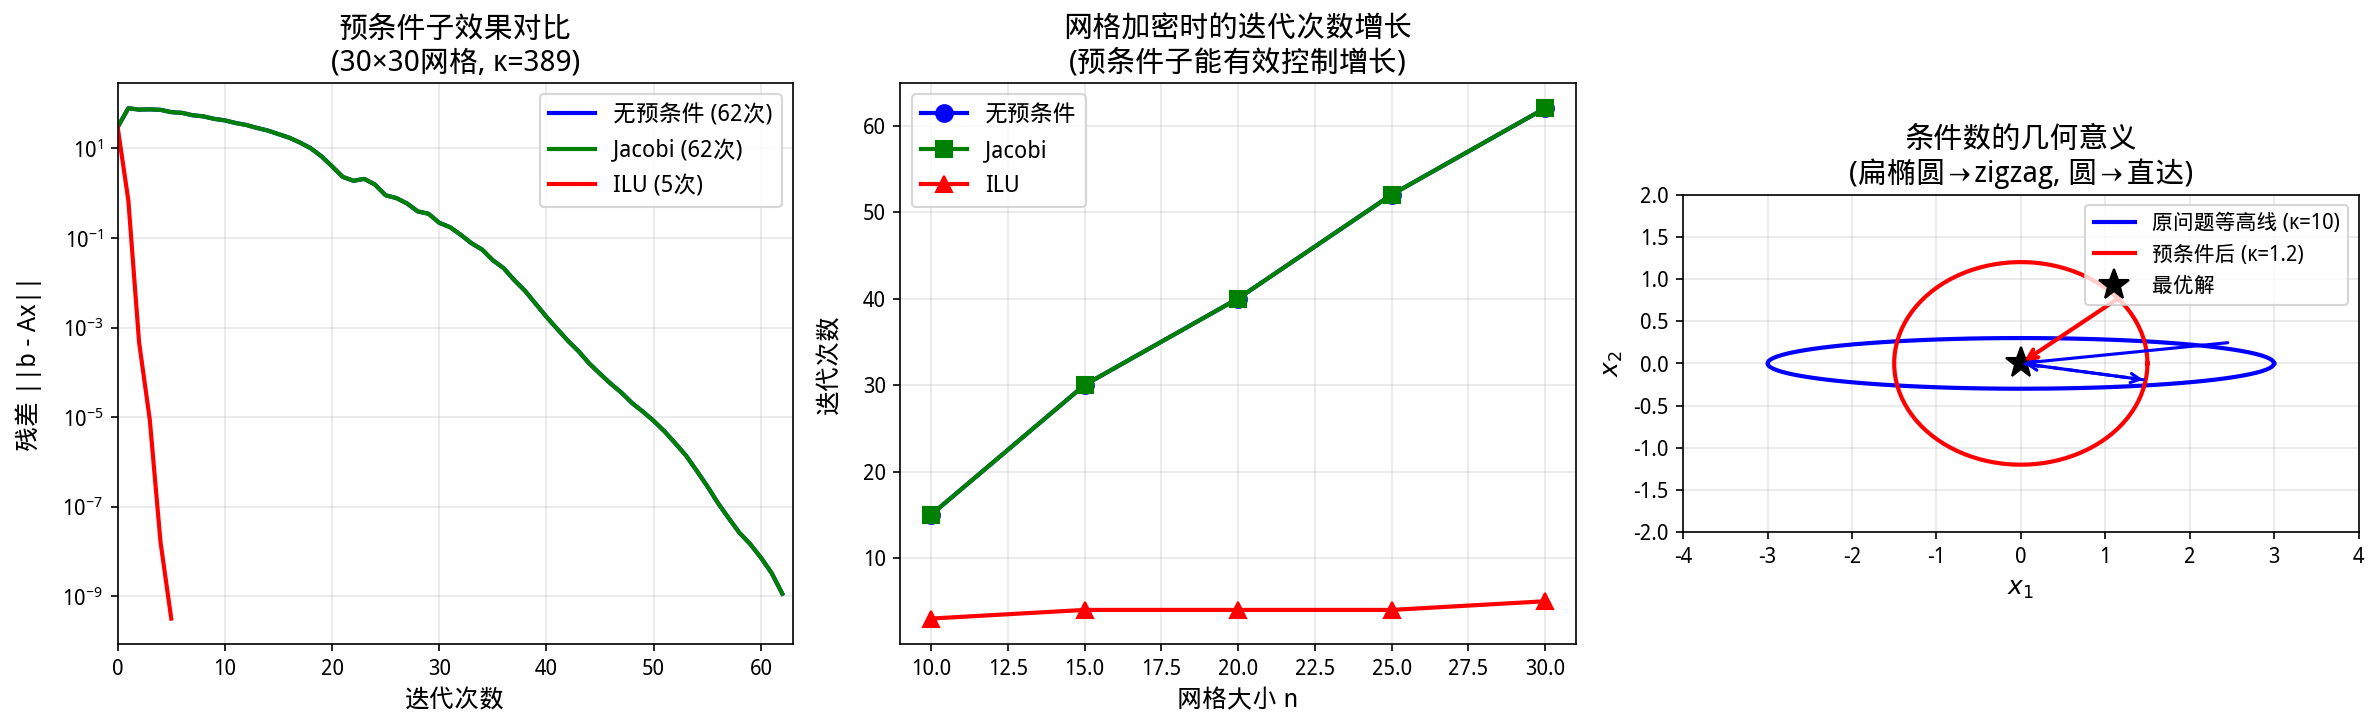
\includegraphics[width=0.95\textwidth]{figs/chap05_fig3.png}
\caption{预条件子效果的实验验证（1行3列）。\textbf{左图}：共轭梯度法收敛曲线对比——无预条件（蓝）、Jacobi预条件（绿）、ILU预条件（红），ILU只需约1/3的迭代次数；\textbf{中图}：网格加密时迭代次数的增长趋势——无预条件和Jacobi迭代次数线性增长，而ILU增长明显更慢；\textbf{右图}：条件数的几何意义——扁椭圆（高条件数）导致zigzag路径，圆形（低条件数）可以直达最优解。代码见 \texttt{code/chap05\_performance.py}。}
\label{fig:preconditioner}
\end{figure}

% ------------------------------------------------------------------------------------
\section*{扩展阅读：CPU 并行计算的真正含义}
\addcontentsline{toc}{section}{扩展阅读：CPU 并行计算的真正含义}

在学习数值计算和科学编程之前，初学者常常会问这样一个问题：

\begin{quote}
"为什么同样是一行代码，有的写法能快几十倍？为什么老师总让我用 NumPy，不要自己写循环？"
\end{quote}

要回答这个问题，我们必须从最基础的地方开始：CPU 是怎样执行程序的？它在什么情况下会变快、在什么情况下会变慢？这部分内容看似属于"计算机系统结构"，但它和我们写出高效代码息息相关。

为了让你真正"看得见"CPU 在做什么，我们会边讲概念边给出小实验。你可以在自己的电脑上立即验证这些现象，而不只是听一堆抽象的术语。

%==============================================================================
\subsection*{程序、进程、线程：你的电脑到底是怎样跑代码的？}
%==============================================================================

我们先从最核心的三个概念讲起。这三个词你可能早就听过，但很多人分不清它们的区别。

\paragraph{程序是什么？}

\textbf{程序（Program）}就是硬盘上的文件——一个 \verb|.exe|、一个 \verb|.py|、一个 \verb|.out|——本质上是一堆指令，静静地躺在那里，还没有执行。

打个比方：程序就像一本菜谱摆在书架上。你不动手做饭，它不会自己飘出味道来。

\paragraph{进程是什么？}

\textbf{进程（Process）}就是程序"开始执行"之后的样子。当你双击一个程序、或者在命令行输入 \verb|python xxx.py| 回车的那一刻，操作系统就会为这个程序创建一个进程。

进程有什么特点呢？它有：
\begin{itemize}
    \item 自己独立的内存空间（别的进程看不到、也改不了）
    \item 自己的变量、数据结构
    \item 自己的一套运行状态
\end{itemize}

继续用做饭来比喻：进程就是"你正在做菜"这件事本身。你占用了一整个厨房，锅、刀、案板、冰箱里的食材，都是你独占的。隔壁厨房在做什么菜，和你没关系。

\paragraph{线程是什么？}

\textbf{线程（Thread）}是进程内部的"执行路线"，或者说是"干活的小工"。一个进程可以同时雇好几个小工，让他们并行地帮你做事。

关键区别在于：同一个进程里的多个线程，\textbf{共享同一片内存空间}。它们可以直接读写同样的变量。

用厨房的比喻来说：
\begin{itemize}
    \item 一个进程是一家餐厅的厨房
    \item 线程是厨房里的多个厨师
    \item 厨师们共享同一个冰箱、同一套锅碗瓢盆（共享内存）
    \item 但不同餐厅的厨房是完全隔开的（进程之间隔离）
\end{itemize}

\begin{figure}[h]
\centering
\begin{tikzpicture}[scale=0.85]
    % 进程1
    \draw[thick, fill=blue!10, rounded corners] (0, 0) rectangle (5, 4);
    \node[font=\bfseries] at (2.5, 3.6) {进程 A（独立内存空间）};
    
    % 内存区域
    \draw[fill=yellow!20] (0.3, 2.2) rectangle (4.7, 3.2);
    \node[font=\small] at (2.5, 2.7) {共享内存：堆、全局变量};
    
    % A 的线程
    \foreach \x/\name in {0.5/线程1,2.1/线程2,3.7/线程3}{
        \draw[fill=green!30] (\x,0.5) rectangle ++(1.3,1.5);
        \node[font=\small, align=center] at (\x+0.65,1.25) {\name\\栈};
    }

    % 进程2
    \draw[thick, fill=red!10, rounded corners] (6, 0) rectangle (11, 4);
    \node[font=\bfseries] at (8.5, 3.6) {进程 B（独立内存空间）};
    \draw[fill=yellow!20] (6.3, 2.2) rectangle (10.7, 3.2);
    \node[font=\small] at (8.5, 2.7) {自己的内存};

    \foreach \x/\name in {6.5/线程1,8.2/线程2,9.9/线程3}{
        \draw[fill=orange!30] (\x,0.5) rectangle ++(1.3,1.5);
        \node[font=\small,align=center] at (\x+0.65,1.25) {\name\\栈};
    }

    % 隔离线
    \draw[ultra thick, red, dashed] (5.5,-0.5) -- (5.5,4.5);
    \node[red, font=\small] at (5.5,-0.8) {内存隔离};
\end{tikzpicture}
\caption{进程与线程的关系：进程之间相互隔离，而同一进程内的线程共享内存}
\end{figure}

下面这张表总结了进程和线程的主要区别：

\begin{center}
\renewcommand{\arraystretch}{1.3}
\begin{tabular}{l|l|l}
\toprule
\textbf{特性} & \textbf{进程} & \textbf{线程} \\
\midrule
内存空间 & 独立，互不共享 & 共享同一进程的内存 \\
创建开销 & 较大（需申请整块内存） & 较小（主要是栈空间） \\
通信方式 & 需要特殊机制（管道、共享内存等） & 直接读写共享变量 \\
崩溃影响 & 一个进程挂了，其他不受影响 & 一个线程挂了，整个进程可能崩溃 \\
典型应用 & 浏览器的多个标签页 & 一个程序内部的并行计算 \\
\bottomrule
\end{tabular}
\end{center}

%------------------------------------------------------------------------------
\paragraph{你可以自己做的小实验 1：Python 多线程为什么不快？}
%------------------------------------------------------------------------------

把下面的代码复制到你的电脑上运行一下：

\begin{lstlisting}[style=teaching, language=Python]
import threading
import time

def count():
    """一个简单的计数任务"""
    n = 0
    for _ in range(50_000_000):
        n += 1

# 先测试单线程
print("测试单线程...")
t0 = time.time()
count()
print(f"单线程耗时: {time.time() - t0:.2f} 秒")

# 再测试双线程
print("\n测试双线程...")
t0 = time.time()
t1 = threading.Thread(target=count)
t2 = threading.Thread(target=count)
t1.start()
t2.start()
t1.join()
t2.join()
print(f"双线程耗时: {time.time() - t0:.2f} 秒")
\end{lstlisting}

运行之后，你大概率会看到一个让人困惑的结果：

\begin{itemize}
    \item 单线程：大约 2--3 秒
    \item 双线程：大约 2--4 秒，甚至更慢！
\end{itemize}

这是怎么回事？开了两个线程，不是应该快一倍吗？

答案是：Python（准确说是 CPython 解释器）有一个特殊的设计叫 \textbf{GIL}（Global Interpreter Lock，全局解释器锁）。它规定：\textbf{同一时刻只能有一个线程在执行 Python 字节码}。

换句话说，即使你开了 10 个线程，Python 解释器也会让它们排队、轮流执行，而不是真正的并行。

这个实验让你亲眼看到了 GIL 的影响。后面我们会讲怎么绑过它。

%==============================================================================
\subsection*{内存层次：为什么有些代码能快 10 倍、100 倍？}
%==============================================================================

当老师说"访问 L1 Cache 是 1 纳秒，访问主内存是 100 纳秒"的时候，初学者往往没有感觉。1 纳秒是什么？100 纳秒又是什么？快还是慢？

我们换一个更直观的比喻。

\marginnote{
\textbf{小故事：}\\
1957 年，IBM 704 计算机的工程师们发现一个问题：CPU 算得太快，常常在"等"内存慢腾腾地把数据送过来。\\
于是他们在 CPU 旁边加了一小块极快的存储器，专门存最近用过的数据——这就是 Cache（高速缓存）的前身。\\
没想到，这个当年的"小补丁"后来成了所有现代处理器的标配设计。
}

想象一下你坐在办公桌前工作：
\begin{itemize}
    \item \textbf{寄存器}（$<1$ ns）：就像你手边的便签纸，伸手就能拿到
    \item \textbf{L1 Cache}（$\sim 1$ ns）：就像桌上的文件夹，抬手就能翻开
    \item \textbf{L2/L3 Cache}（几 ns--十几 ns）：就像抽屉里的资料，需要弯腰去拿
    \item \textbf{主内存 RAM}（$\sim 100$ ns）：就像走去隔壁房间的档案柜取文件
    \item \textbf{SSD 硬盘}（$\sim 100$ $\mu$s）：就像开车去另一栋楼的仓库取东西
\end{itemize}

现在你明白了吧？如果你的程序总是要"开车去仓库"，而别人的程序只需要"翻桌上的文件夹"，速度差别当然是天壤之别。

\begin{center}
\renewcommand{\arraystretch}{1.3}
\begin{tabular}{l|r|r|l}
\toprule
\textbf{层次} & \textbf{延迟（量级）} & \textbf{容量} & \textbf{类比} \\
\midrule
寄存器 & $< 1$ ns & 几十个字 & 手边的便签纸 \\
L1 Cache & $\sim 1$ ns & 32--64 KB & 桌上的文件夹 \\
L2/L3 Cache & 几--十几 ns & 数百 KB--数十 MB & 抽屉、柜子 \\
主内存（RAM） & $\sim 100$ ns & GB 级 & 隔壁房间档案室 \\
SSD & $\sim 100$ $\mu$s & TB 级 & 另一栋楼的仓库 \\
\bottomrule
\end{tabular}
\end{center}

这就引出了一个极其重要的概念：\textbf{数据局部性（Data Locality）}。

所谓数据局部性，就是说：如果你的程序访问的数据"挨在一起"，CPU 就能把它们一起搬进 Cache，后续访问就会非常快。反过来，如果你的程序东一下西一下地乱跳着访问数据，CPU 就不得不频繁地去"隔壁房间取文件"，速度就会慢很多。

%------------------------------------------------------------------------------
\paragraph{你可以自己做的小实验 2：按行访问 vs 按列访问}
%------------------------------------------------------------------------------

下面这个实验非常经典，能让你直观地"看见"Cache 的影响：

\begin{lstlisting}[style=teaching, language=Python]
import numpy as np
import time

N = 5000
A = np.random.rand(N, N)

# 方式一：按行访问（先固定 i，再遍历 j）
print("测试按行访问...")
t0 = time.time()
s = 0.0
for i in range(N):
    for j in range(N):
        s += A[i, j]
print(f"按行访问: {time.time() - t0:.2f} 秒")

# 方式二：按列访问（先固定 j，再遍历 i）
print("\n测试按列访问...")
t0 = time.time()
s = 0.0
for j in range(N):
    for i in range(N):
        s += A[i, j]
print(f"按列访问: {time.time() - t0:.2f} 秒")
\end{lstlisting}

运行之后，你会看到一个惊人的结果：

\begin{itemize}
    \item 按行访问：大约 5--8 秒
    \item 按列访问：大约 15--40 秒，慢了好几倍！
\end{itemize}

这两段代码做的事情完全一样——都是把矩阵所有元素加起来。循环次数也完全一样。为什么速度差这么多？

原因就在于 \textbf{NumPy 默认按行存储矩阵}（所谓 row-major order）。也就是说，\verb|A[0,0], A[0,1], A[0,2], ...| 这些元素在内存中是连续存放的。

当你按行访问时，CPU 读取 \verb|A[0,0]| 的同时，会顺便把 \verb|A[0,1], A[0,2], ...| 等一串数据都搬进 Cache。接下来你访问 \verb|A[0,1]| 时，它已经在 Cache 里了，不需要再去主内存取。

但当你按列访问时，你先访问 \verb|A[0,0]|，下一个却要访问 \verb|A[1,0]|——这两个数据在内存中相隔很远！CPU 刚搬进来的那一串数据全都用不上，又得重新去主内存取。这就是为什么按列访问会慢那么多。

\paragraph{结论：写数值代码时应该这样做}

\begin{itemize}
    \item 尽量让数据\textbf{连续存放}，按顺序访问（比如按行遍历矩阵）
    \item 尽量\textbf{少做随机跳跃式}的访问
    \item 能在一次循环里完成的事情，就不要拆成好几个循环，每次都重新扫描整个大数组
\end{itemize}

%==============================================================================
\subsection*{Python 的 GIL：为什么多线程常常"白忙活"？}
%==============================================================================

前面的实验已经让你看到了：Python 多线程在纯计算任务上并不能加速。现在我们来仔细解释一下原因。

\begin{definition}[全局解释器锁 GIL]
GIL（Global Interpreter Lock）是 CPython 解释器中的一个互斥锁。它的作用是：\textbf{保证同一时刻只有一个线程在执行 Python 字节码}。
\end{definition}

\begin{remark}
值得一提的是，Python 3.13（2024 年发布）开始提供"无 GIL"的实验性构建版本（称为 free-threaded 模式）。这意味着未来的 Python 有望真正支持多线程并行计算。不过，由于目前大多数生产环境和教学场景仍在使用 Python 3.10--3.12，而且许多第三方库尚未完全适配无 GIL 版本，本书仍以传统的带 GIL 的 Python 为基础进行讲解。当你阅读本书时，如果 Python 的无 GIL 版本已经成熟普及，下面关于"多线程无法加速计算密集型任务"的讨论可能就不再适用了——但理解 GIL 的历史和原理，仍然有助于你理解 Python 的设计哲学和大量遗留代码的行为。
\end{remark}

为什么 Python 要设计这么一个"奇怪"的锁呢？历史原因是：Python 的内存管理（特别是引用计数）不是线程安全的。如果允许多个线程同时修改 Python 对象，可能会导致内存错误。GIL 是一个简单粗暴但有效的解决方案。

GIL 的直接后果是：

\begin{itemize}
    \item 对于 \textbf{IO 密集型任务}（比如网络请求、读写文件），多线程仍然有用。因为当一个线程在等待 IO 时，它会释放 GIL，让其他线程有机会执行。
    \item 对于 \textbf{CPU 计算密集型任务}（比如大量数学运算），多线程基本没用。因为所有线程都在抢同一把锁，轮流执行，跟单线程没什么区别。
\end{itemize}

%------------------------------------------------------------------------------
\paragraph{那 Python 就没法并行计算了吗？}
%------------------------------------------------------------------------------

当然不是。有好几种方法可以绑过 GIL 的限制：

\begin{center}
\renewcommand{\arraystretch}{1.3}
\begin{tabular}{l|l|l}
\toprule
\textbf{方法} & \textbf{怎么做} & \textbf{适合什么场景} \\
\midrule
多进程 & 用 \verb|multiprocessing| 模块 & 计算密集型任务 \\
NumPy/SciPy & 调用底层 C/Fortran 库 & 数值计算（强烈推荐） \\
Numba/Cython & 把 Python 代码编译成机器码 & 热点代码加速 \\
异步 IO & 用 \verb|asyncio| 模块 & 网络、文件 IO \\
\bottomrule
\end{tabular}
\end{center}

对于初学者来说，最实用的建议是：

\begin{enumerate}
    \item \textbf{数值计算优先用 NumPy}，而不是自己写 Python 循环。NumPy 的底层是 C 代码，不受 GIL 限制。
    \item 如果确实需要用多核并行，可以用 \verb|multiprocessing.Pool|：
\end{enumerate}

\begin{lstlisting}[style=teaching, language=Python]
from multiprocessing import Pool
import time

def heavy_compute(x):
    """一个耗时的计算任务"""
    return sum(i * i for i in range(x))

if __name__ == "__main__":
    numbers = list(range(1000, 2000))
    
    # 单进程
    t0 = time.time()
    results1 = [heavy_compute(x) for x in numbers]
    print(f"单进程: {time.time() - t0:.2f} 秒")
    
    # 多进程（4 个工作进程）
    t0 = time.time()
    with Pool(processes=4) as pool:
        results2 = pool.map(heavy_compute, numbers)
    print(f"多进程: {time.time() - t0:.2f} 秒")
\end{lstlisting}

运行这段代码，你会发现多进程版本确实快了好几倍——因为每个进程有自己独立的 Python 解释器和 GIL，它们可以真正地并行执行。

%==============================================================================
\subsection*{NumPy 为什么比"纯 Python"快？}
%==============================================================================

很多老师会说："\textbf{不要自己写 for 循环，尽量用 NumPy。}" 这句话背后的原因到底是什么？

主要有三条：

\paragraph{原因 1：底层是 C/Fortran 代码，没有解释器开销}

当你写一个 Python 循环时，解释器需要一行一行地"翻译"和执行。每一次循环迭代都有额外的开销：检查类型、查找变量、更新计数器……

\begin{lstlisting}[style=teaching, language=Python]
# 纯 Python：一百万次循环，解释器忙个不停
c = [a[i] + b[i] for i in range(1_000_000)]

# NumPy：一行代码，底层用 C 循环执行
c = a + b
\end{lstlisting}

第二行看起来很短，但它在底层做了很多事情：用 C 语言写的循环、没有 Python 解释器的开销、而且可以利用各种硬件优化。

\paragraph{原因 2：可以使用 SIMD 指令}

现代 CPU 有一类特殊的指令叫 SIMD（Single Instruction, Multiple Data）。顾名思义，一条指令可以同时处理多个数据。比如，一条 AVX 指令可以同时对 8 个浮点数做加法。

你在 Python 层面是看不到这些指令的，但 NumPy 底层的 C 代码会自动利用它们。

\paragraph{原因 3：底层库已经做好了多线程和 Cache 优化}

NumPy 的矩阵运算实际上调用的是 BLAS（Basic Linear Algebra Subprograms）库。这些库是几十年来无数专家精心优化的结晶，包括：

\begin{itemize}
    \item 自动把大矩阵分块，让每一块都能装进 Cache
    \item 自动开多线程，用满 CPU 的所有核心
    \item 针对不同 CPU 架构做专门优化
\end{itemize}

%------------------------------------------------------------------------------
\paragraph{你可以自己做的小实验 3：}感受 NumPy 的速度
%------------------------------------------------------------------------------

\begin{lstlisting}[style=teaching, language=Python]
import numpy as np
import time

# 准备数据：500 万个随机数
x = np.random.rand(5_000_000)
y = np.random.rand(5_000_000)

# 方式一：纯 Python 循环
print("测试纯 Python...")
t0 = time.time()
z1 = [x[i] + y[i] for i in range(5_000_000)]
print(f"纯 Python: {time.time() - t0:.3f} 秒")

# 方式二：NumPy 向量运算
print("\n测试 NumPy...")
t0 = time.time()
z2 = x + y
print(f"NumPy: {time.time() - t0:.3f} 秒")
\end{lstlisting}

运行结果大概是：

\begin{itemize}
    \item 纯 Python：0.3--0.5 秒
    \item NumPy：0.005--0.01 秒
\end{itemize}

快了 \textbf{几十倍}！而且代码还更简洁。这就是为什么老师总让你用 NumPy。

\paragraph{对你来说最实用的一句总结}

如果你写的是数值计算代码，优先想一想："\textbf{这个能不能写成 NumPy 的数组运算？}" 能用数组运算，就别写 Python 层的 for 循环。

%==============================================================================
\subsection*{CPU 与 GPU 的对比：不同的设计哲学}
%==============================================================================

最后，我们来简单聊聊 CPU 和 GPU 的区别。这个话题以后学深度学习时会深入讨论，这里先建立一个基本印象。

\paragraph{一句话总结}

\begin{quote}
CPU 是一个非常聪明的工人，能处理各种复杂任务。\\
GPU 是一大群比较简单的工人，但人多力量大。
\end{quote}

\paragraph{CPU 的设计哲学}

CPU 的核心数量不多（通常 4--64 个），但每个核心都非常强大：

\begin{itemize}
    \item 复杂的控制逻辑，能处理各种 if-else 分支
    \item 乱序执行、分支预测等高级优化
    \item 大容量的 Cache
\end{itemize}

CPU 擅长处理：流程复杂、分支很多、任务各不相同的程序。比如操作系统、编译器、数据库等。

\paragraph{GPU 的设计哲学}

GPU 的核心数量非常多（上千个），但每个核心都比较简单：

\begin{itemize}
    \item 简单的算术逻辑单元，擅长做加法、乘法
    \item 不擅长处理复杂的控制流
    \item 极高的内存带宽
\end{itemize}

GPU 擅长处理：同一种运算要作用在大量数据上的任务。比如矩阵乘法、图像处理、物理模拟等。

\begin{center}
\renewcommand{\arraystretch}{1.3}
\begin{tabular}{l|l|l}
\toprule
\textbf{特性} & \textbf{CPU} & \textbf{GPU} \\
\midrule
核心数量 & 少（4--64） & 多（数千） \\
单核能力 & 强（复杂控制逻辑） & 弱（简单算术运算） \\
擅长任务 & 分支多、流程复杂 & 大规模并行计算 \\
内存带宽 & 较低 & 非常高 \\
编程难度 & 低 & 较高 \\
\bottomrule
\end{tabular}
\end{center}

%------------------------------------------------------------------------------
\paragraph{你可以自己做的小实验 4：CPU vs GPU 矩阵乘法}
%------------------------------------------------------------------------------

如果你的电脑有 NVIDIA 显卡，可以试试下面的代码（需要安装 PyTorch）：

\begin{lstlisting}[style=teaching, language=Python]
import torch
import time

# 准备两个大矩阵
A = torch.randn(4000, 4000)
B = torch.randn(4000, 4000)

# CPU 版本
print("测试 CPU...")
t0 = time.time()
C_cpu = A @ B
print(f"CPU: {time.time() - t0:.3f} 秒")

# GPU 版本（如果有 CUDA）
if torch.cuda.is_available():
    A_gpu = A.cuda()
    B_gpu = B.cuda()
    
    # 预热
    _ = A_gpu @ B_gpu
    torch.cuda.synchronize()
    
    print("\n测试 GPU...")
    t0 = time.time()
    C_gpu = A_gpu @ B_gpu
    torch.cuda.synchronize()
    print(f"GPU: {time.time() - t0:.3f} 秒")
else:
    print("\n（没有检测到 CUDA，跳过 GPU 测试）")
\end{lstlisting}

如果你有 GPU，会看到类似这样的结果：

\begin{itemize}
    \item CPU：1--3 秒
    \item GPU：0.01--0.05 秒
\end{itemize}

快了 \textbf{几十倍到上百倍}！这就是为什么深度学习训练几乎都在 GPU 上进行。

%==============================================================================
\subsection*{并行计算的层次结构}
%==============================================================================

到这里，我们可以把并行计算的各种层次整理一下：

\begin{figure}[h]
\centering
\begin{tikzpicture}[
    box/.style={draw, rounded corners, minimum width=4.5cm, minimum height=0.9cm, font=\small, align=center},
    scale=0.95
]
    \node[box, fill=red!20] at (0, 4.5) {指令级并行（ILP）\\CPU 硬件自动完成};
    \node[box, fill=orange!20] at (0, 3.0) {数据级并行（SIMD）\\NumPy、向量指令};
    \node[box, fill=yellow!20] at (0, 1.5) {线程/进程级并行\\多线程、多进程};
    \node[box, fill=green!20] at (0, 0) {节点级并行\\多机集群、MPI};
    
    \draw[<->, thick] (-3.2, -0.3) -- (-3.2, 4.8);
    \node[left, font=\small, rotate=90] at (-3.5, 2.25) {粒度：从细到粗};
    
    \draw[<->, thick] (3.2, -0.3) -- (3.2, 4.8);
    \node[right, font=\small, rotate=270] at (3.5, 2.25) {编程难度：从低到高};
\end{tikzpicture}
\caption{并行计算的层次：越往上粒度越细，通常由硬件或编译器自动完成；越往下粒度越粗，需要程序员手动管理}
\end{figure}

对于初学者来说：

\begin{itemize}
    \item \textbf{指令级并行}：你不需要管，CPU 会自动做
    \item \textbf{数据级并行}：用 NumPy 就能享受到，不需要自己写
    \item \textbf{线程/进程级并行}：需要时可以用 \verb|multiprocessing|
    \item \textbf{节点级并行}：等你以后做大规模计算再学
\end{itemize}

%==============================================================================
\subsection*{本节小结：给你的实践建议}
%==============================================================================

第一次接触这些概念的读者，应该记住以下几点：

\begin{enumerate}
    \item \textbf{写数值代码时，优先用 NumPy}，而不是纯 Python 循环。这一条最重要。
    
    \item \textbf{注意数据的访问模式}。尽量让数据连续存放、按顺序访问。避免随机跳跃式的访问。
    
    \item \textbf{Python 多线程对 CPU 密集型任务没用}，因为 GIL 的存在。需要多核并行时，用多进程。
    
    \item \textbf{当程序变慢时}，不要第一反应怪"电脑太差"。先想想：
    \begin{itemize}
        \item 是不是在用 Python 循环遍历大数组？
        \item 是不是内存访问模式很"跳跃"？
        \item 是不是开了很多线程但被 GIL 卡住？
    \end{itemize}
    
    \item \textbf{GPU 适合大规模并行计算}（比如矩阵运算），CPU 适合复杂逻辑。以后遇到"同一种计算要做几百万次"的任务，就可以考虑用 GPU。
\end{enumerate}

掌握这些基础概念，你以后再学操作系统、计算机体系结构、并行计算课程时会轻松很多。而且从现在开始，你就可以写出\textbf{更快、更高效}的数值计算代码了。


% ====================================================================================
\section*{扩展阅读：流固耦合有限元——Turek-Hron FSI2基准测试}
\addcontentsline{toc}{section}{扩展阅读：流固耦合有限元}
% ====================================================================================

\begin{tcolorbox}[colback=gray!5, colframe=gray!50, title=本节导读]
你有没有见过大风中摇晃的旗杆？或者听说过塔科马海峡大桥在风中剧烈扭曲最终坍塌的故事？

这些现象背后有一个共同的物理机制：\textbf{流固耦合}（Fluid-Structure Interaction, FSI）。流体（空气或水）作用于固体结构，固体的变形又反过来影响流场，形成复杂的相互作用。

本节介绍流固耦合领域最著名的基准测试——\textbf{Turek-Hron FSI2问题}：一个弹性薄板固连在圆柱后方，在来流作用下发生大幅度自激振荡。这个问题展示了涡激振动的典型特征，也是验证FSI求解器的工业标准。
\end{tcolorbox}

% ------------------------------------------------------------------------------------
\subsection*{一、问题描述：圆柱后的弹性旗}

Turek和Hron在2006年提出了一系列FSI基准测试问题，其中\textbf{FSI2}是最具挑战性也最常被引用的一个。

\begin{figure}[h]
\centering
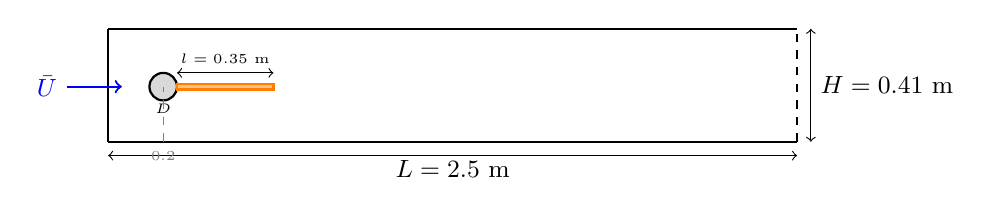
\begin{tikzpicture}[scale=3.5]
    % 通道
    \draw[thick] (0,0) -- (2.5,0);
    \draw[thick] (0,0.41) -- (2.5,0.41);

    % 入口
    \draw[thick] (0,0) -- (0,0.41);
    \draw[->, blue, thick] (-0.15,0.2) -- (0.05,0.2);
    \node[blue, left] at (-0.15,0.2) {\small $\bar{U}$};

    % 出口
    \draw[thick, dashed] (2.5,0) -- (2.5,0.41);

    % 圆柱
    \fill[gray!30] (0.2,0.2) circle (0.05);
    \draw[thick] (0.2,0.2) circle (0.05);
    \node at (0.2,0.12) {\tiny $D$};

    % 弹性板
    \fill[orange!50] (0.25,0.19) rectangle (0.6,0.21);
    \draw[thick, orange] (0.25,0.19) -- (0.6,0.19) -- (0.6,0.21) -- (0.25,0.21) -- cycle;

    % 标注
    \draw[<->] (0,-0.05) -- (2.5,-0.05);
    \node at (1.25,-0.1) {\small $L = 2.5$ m};
    \draw[<->] (2.55,0) -- (2.55,0.41);
    \node[right] at (2.55,0.205) {\small $H = 0.41$ m};

    % 板的标注
    \draw[<->] (0.25,0.25) -- (0.6,0.25);
    \node[above] at (0.425,0.25) {\tiny $l = 0.35$ m};

    % 圆心位置
    \draw[dashed, gray] (0.2,0) -- (0.2,0.2);
    \node[gray, below] at (0.2,0) {\tiny 0.2};
\end{tikzpicture}
\caption{Turek-Hron FSI2几何设置。矩形通道（$2.5 \times 0.41$ m）内有一刚性圆柱（直径$D = 0.1$ m），圆心在$(0.2, 0.2)$m处（故意偏心以打破对称性）。一块弹性薄板（长$0.35$ m，厚$0.02$ m，橙色）固连在圆柱后方。流体从左侧入口以抛物线速度剖面进入。}
\label{fig:turek_fsi_geometry}
\end{figure}

\paragraph{物理参数}

\begin{center}
\renewcommand{\arraystretch}{1.3}
\begin{tabular}{l|l|l}
\toprule
\textbf{参数} & \textbf{符号} & \textbf{FSI2取值} \\
\midrule
流体密度 & $\rho_f$ & 1000 kg/m³ \\
动力粘度 & $\mu_f$ & 0.001 Pa$\cdot$s \\
平均入口速度 & $\bar{U}$ & 1.0 m/s \\
雷诺数 & Re $= \rho_f \bar{U} D / \mu_f$ & 100 \\
\midrule
固体密度 & $\rho_s$ & 10000 kg/m³ \\
杨氏模量 & $E$ & $1.4 \times 10^6$ Pa \\
泊松比 & $\nu_s$ & 0.4 \\
\midrule
密度比 & $\rho_s / \rho_f$ & 10 \\
\bottomrule
\end{tabular}
\end{center}

\begin{marginnote}
\textbf{为什么圆心偏心？} 如果圆柱在通道正中央，由于对称性，初始阶段不会产生涡脱落。偏心打破了对称性，使得流动从一开始就不稳定，更快进入周期性振荡状态。
\end{marginnote}

% ------------------------------------------------------------------------------------
\subsection*{二、涡激振动机理}

当流体绕过圆柱时，会在圆柱两侧交替脱落旋转方向相反的涡——这就是著名的\textbf{卡门涡街}（Kármán vortex street）。

\begin{marginnote}
\textbf{西奥多·冯·卡门}（Theodore von Kármán, 1881--1963）是20世纪最伟大的航空工程师之一。他不仅发现了卡门涡街，还创立了喷气推进实验室（JPL），培养了钱学森等众多杰出学生。
\end{marginnote}

\begin{figure}[htbp]
\centering
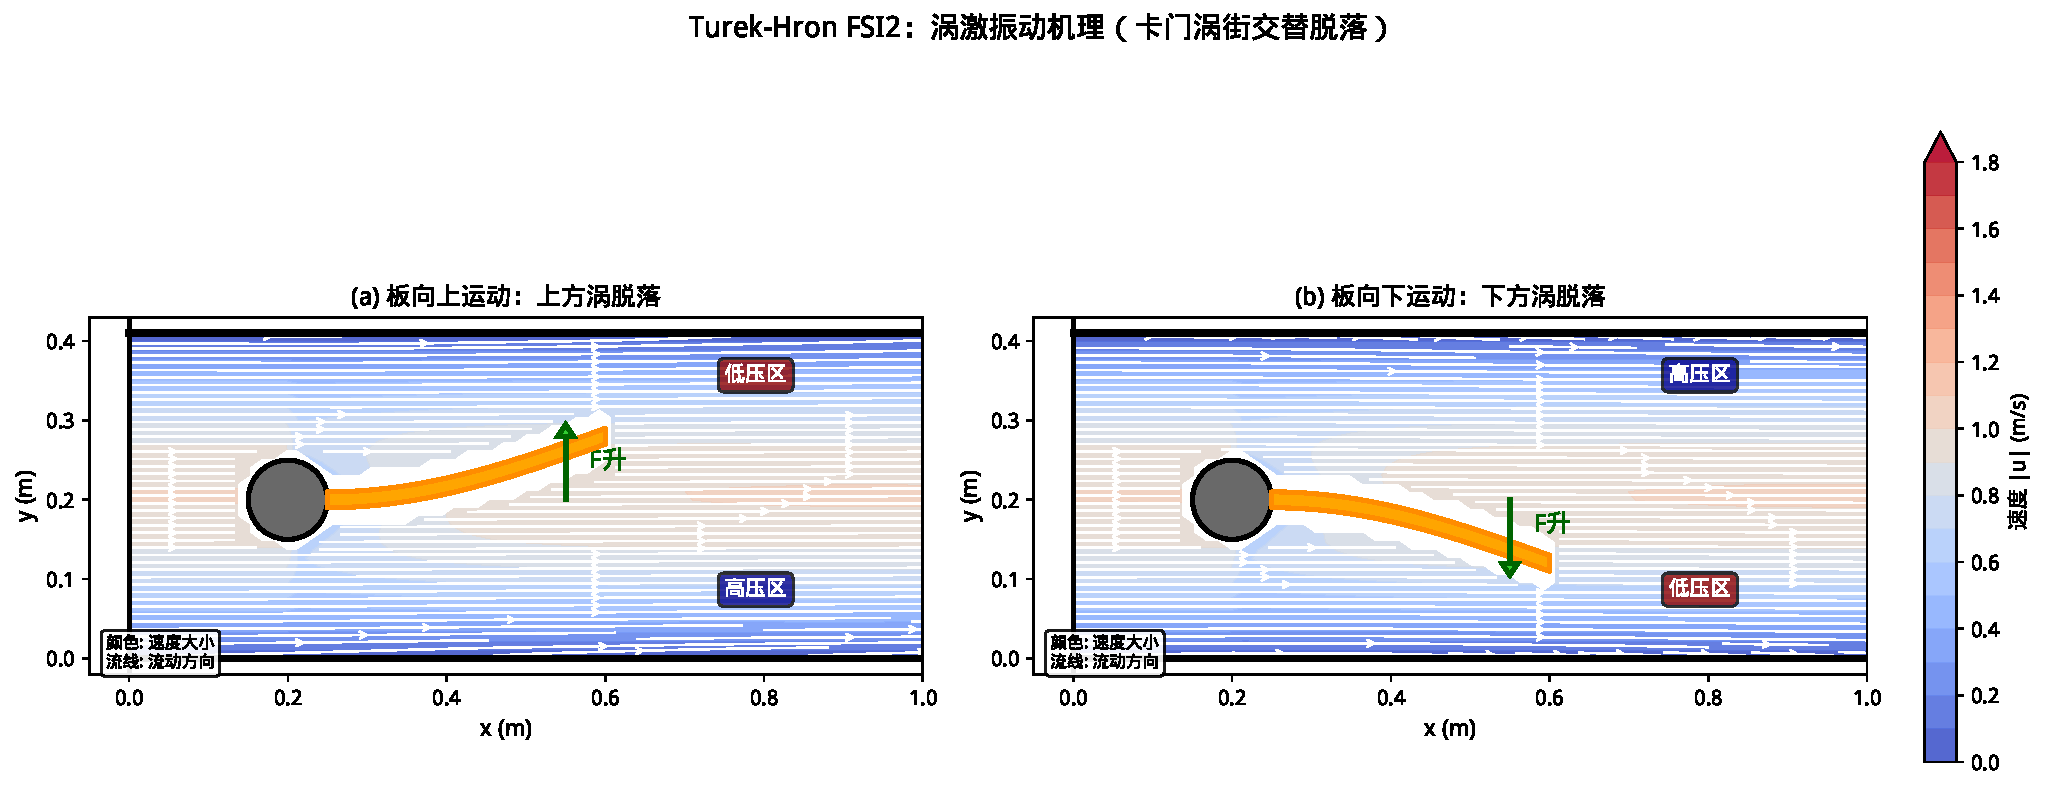
\includegraphics[width=0.98\textwidth]{figs_chap05/turek_fsi2_mechanism.pdf}
\caption{涡激振动机理示意。(a) 当上方涡脱落时，圆柱和板上方形成低压区，产生向上的升力，推动弹性板向上弯曲。(b) 半个周期后，下方涡脱落，下方形成低压区，产生向下的升力。这种交替的压力差驱动板的周期性振荡。}
\label{fig:turek_fsi2_mechanism}
\end{figure}

涡脱落频率由\textbf{Strouhal数}确定：
\begin{equation}
f_s = \text{St} \cdot \frac{U}{D}
\end{equation}
其中$\text{St} \approx 0.2$对于许多钝体都近似成立。对于FSI2条件：$f_s \approx 0.2 \times 1.0 / 0.1 = 2$ Hz。

当这个涡脱落频率接近弹性板的固有频率时，会发生\textbf{锁定}（lock-in）现象：
\begin{itemize}
    \item 涡脱落频率被"锁定"到结构固有频率
    \item 振幅急剧增大
    \item 流固相互作用形成正反馈，系统进入\textbf{自激振荡}
\end{itemize}

% ------------------------------------------------------------------------------------
\subsection*{三、振动响应}

经过初始瞬态后，弹性板进入稳态周期振荡。图\ref{fig:turek_fsi2_snapshots}展示了一个振动周期内弹性板的变形序列。

\begin{figure}[htbp]
\centering
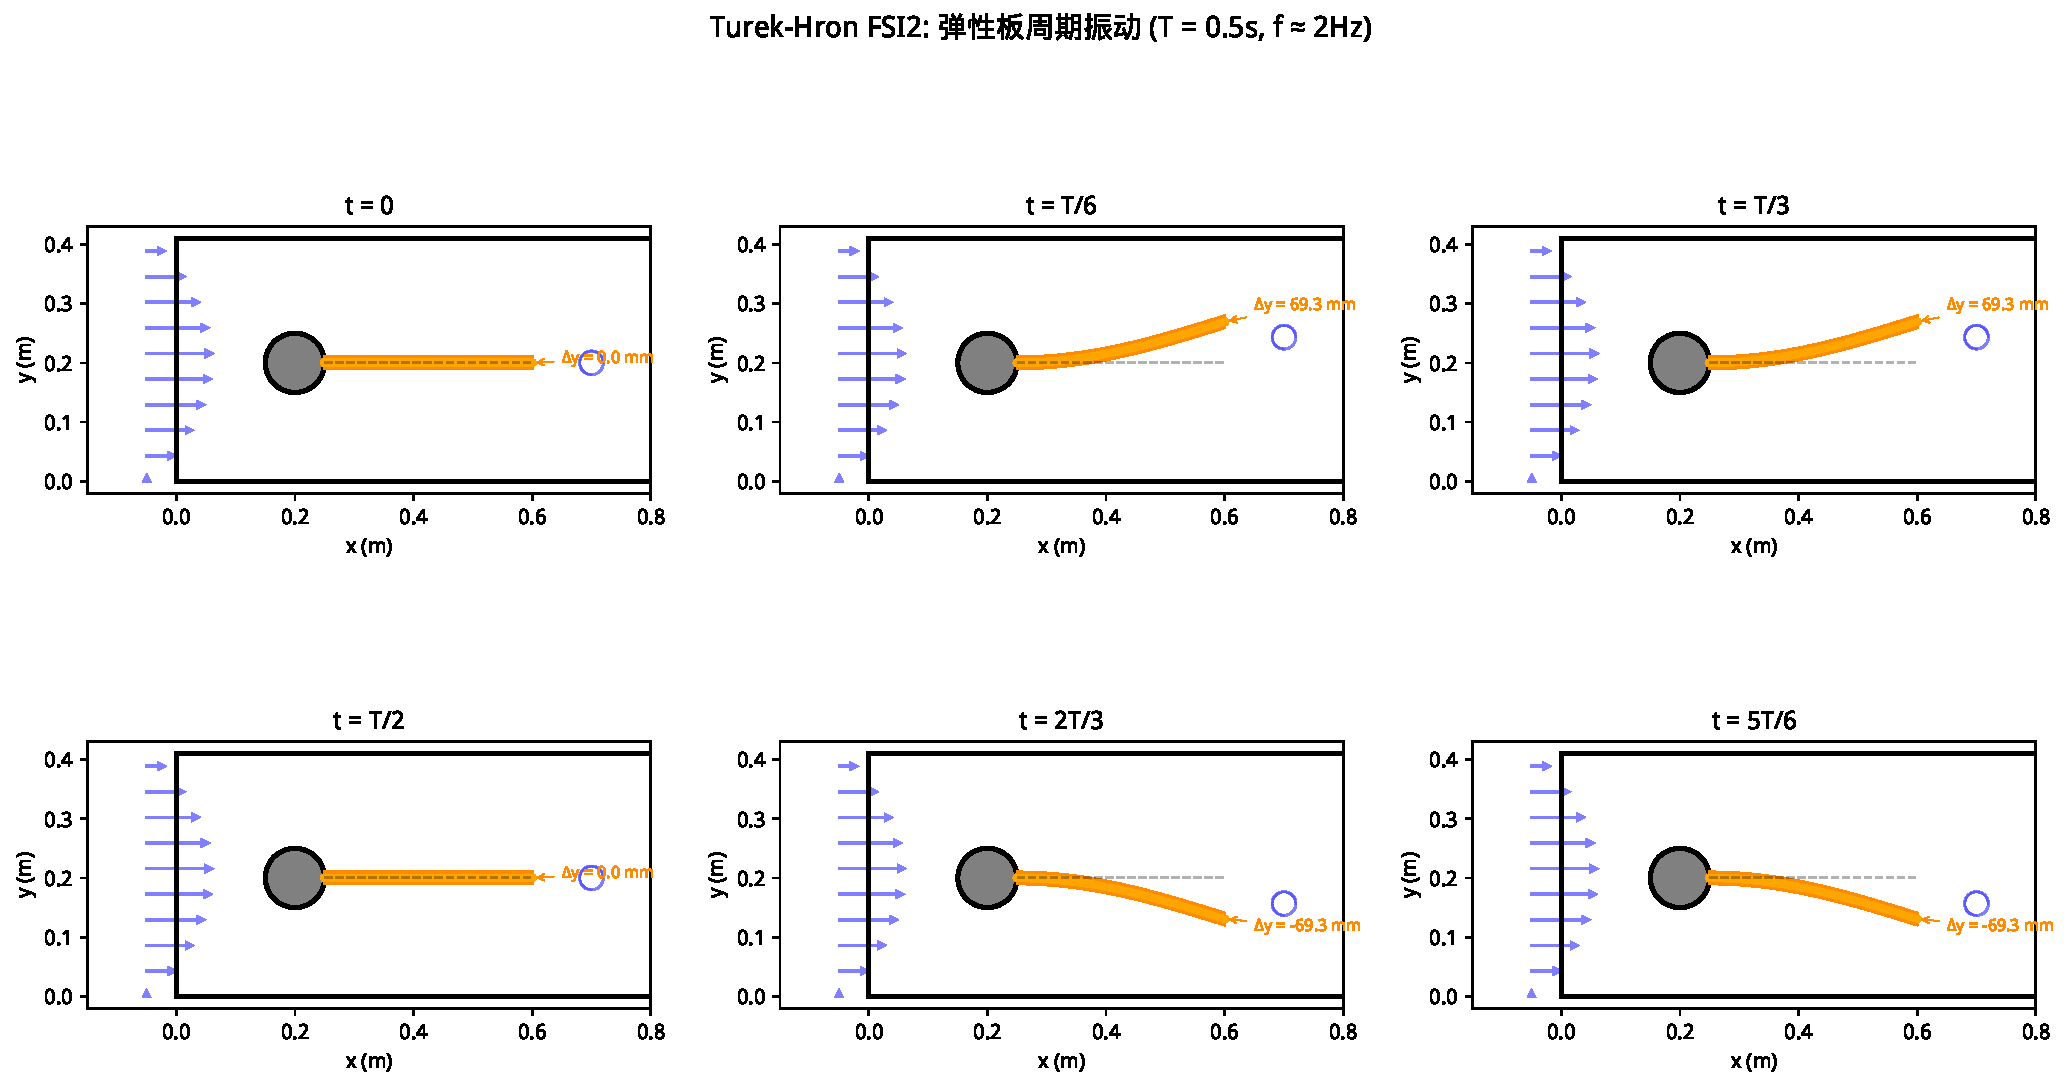
\includegraphics[width=0.98\textwidth]{figs_chap05/turek_fsi2_snapshots.pdf}
\caption{Turek-Hron FSI2：弹性板在一个振动周期（$T \approx 0.5$ s）内的变形快照。板端Y方向位移幅值约$\pm 80$ mm，这是板长（350 mm）的约23\%——属于大变形范畴！注意板的变形主要由一阶弯曲模态主导。}
\label{fig:turek_fsi2_snapshots}
\end{figure}

图\ref{fig:turek_fsi2_analysis}给出了完整的动力学分析。

\begin{figure}[htbp]
\centering
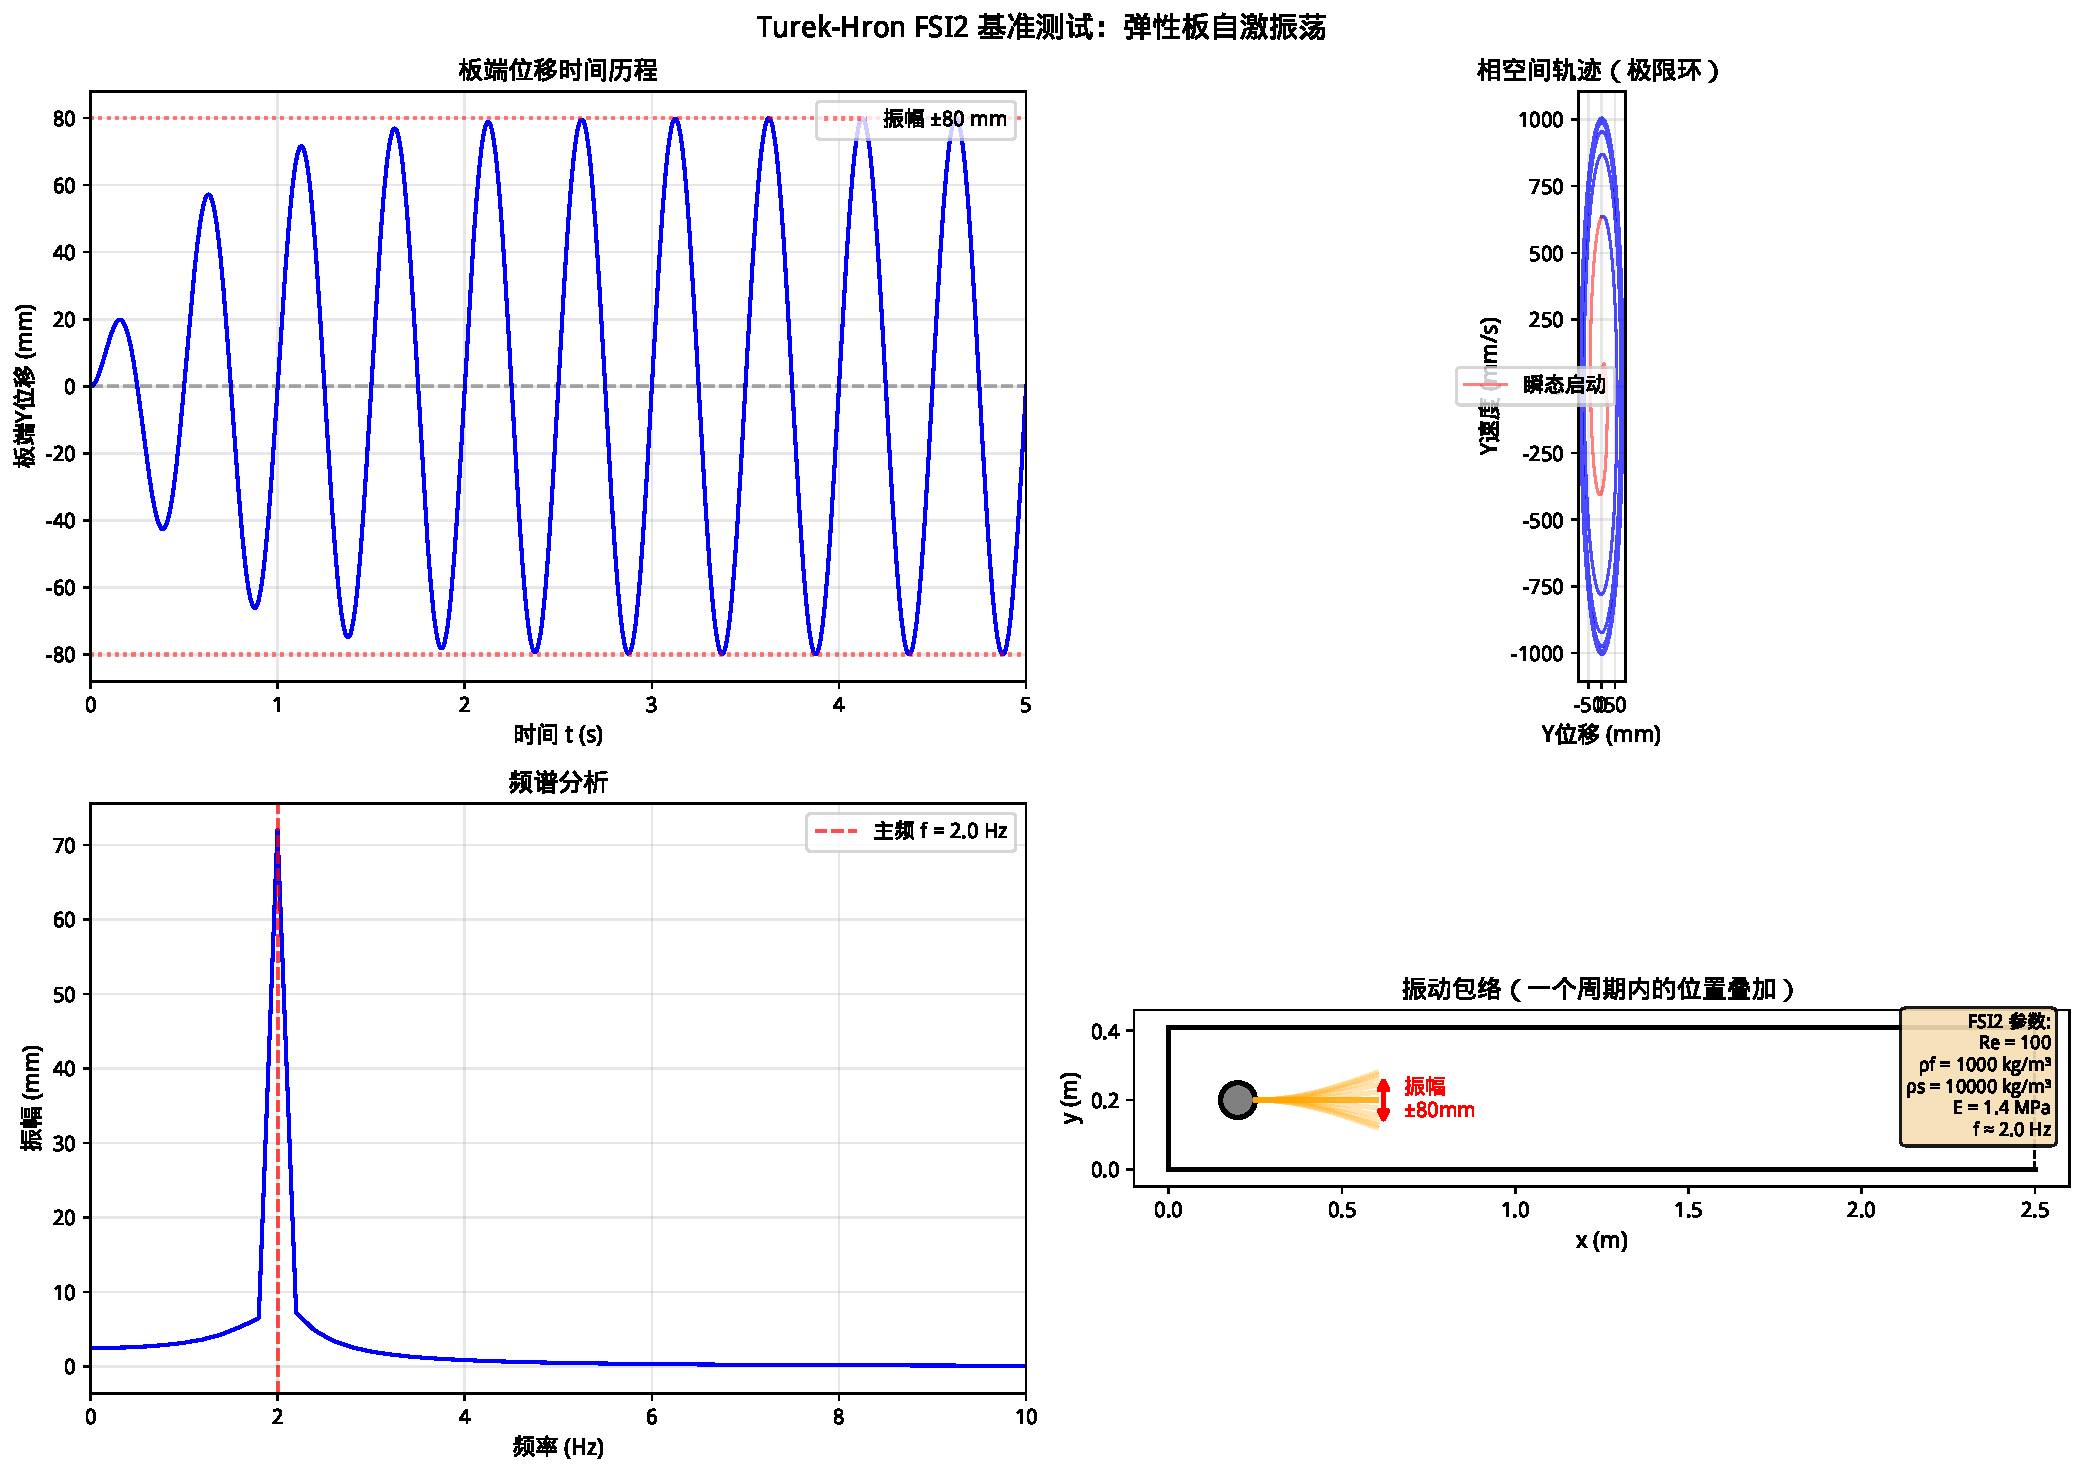
\includegraphics[width=0.98\textwidth]{figs_chap05/turek_fsi2_time_history.pdf}
\caption{Turek-Hron FSI2动力学分析。\textbf{左上}：板端Y位移时间历程——经过短暂瞬态后进入稳态振荡，振幅约$\pm 80$ mm。\textbf{右上}：相空间轨迹——稳态时形成极限环（limit cycle），这是自激振荡的标志。\textbf{左下}：频谱分析——主频约2 Hz，与涡脱落频率一致。\textbf{右下}：振动包络——一个周期内板的位置叠加，展示振动的空间范围。}
\label{fig:turek_fsi2_analysis}
\end{figure}

\paragraph{文献参考值}
Turek和Hron报告的FSI2基准结果：
\begin{itemize}
    \item 板端Y方向位移：$y(A) = 1.23 \pm 80.6 \times 10^{-3}$ m（均值1.23 mm，振幅80.6 mm）
    \item 振动频率：$f \approx 2.0$ Hz
    \item 圆柱阻力系数：$C_D = 208.83 \pm 73.75$
    \item 圆柱升力系数：$C_L = 0.88 \pm 234.2$
\end{itemize}

% ------------------------------------------------------------------------------------
\subsection*{四、结构建模：Euler-Bernoulli梁有限元}

弹性板可以用\textbf{Euler-Bernoulli梁理论}建模。控制方程为：
\begin{equation}
EI \frac{\partial^4 w}{\partial x^4} + \rho A \frac{\partial^2 w}{\partial t^2} = f(x, t)
\end{equation}
其中$w(x,t)$是横向位移，$EI$是抗弯刚度，$\rho A$是单位长度质量，$f(x,t)$是流体力。

\subsubsection*{单元刚度矩阵与质量矩阵}

对于长度为$L_e$的梁单元，每端有两个自由度（位移$w$和转角$\theta$），单元矩阵是$4 \times 4$的：
\begin{equation}
\mathbf{K}_e = \frac{EI}{L_e^3}
\begin{pmatrix}
12 & 6L_e & -12 & 6L_e \\
6L_e & 4L_e^2 & -6L_e & 2L_e^2 \\
-12 & -6L_e & 12 & -6L_e \\
6L_e & 2L_e^2 & -6L_e & 4L_e^2
\end{pmatrix}, \quad
\mathbf{M}_e = \frac{\rho A L_e}{420}
\begin{pmatrix}
156 & 22L_e & 54 & -13L_e \\
22L_e & 4L_e^2 & 13L_e & -3L_e^2 \\
54 & 13L_e & 156 & -22L_e \\
-13L_e & -3L_e^2 & -22L_e & 4L_e^2
\end{pmatrix}
\end{equation}

\begin{marginnote}
\textbf{注意}：FSI2涉及大变形，严格来说需要使用几何非线性公式（如协同旋转法或Total Lagrangian公式）。这里的线性梁模型只是演示目的。
\end{marginnote}

% ------------------------------------------------------------------------------------
\subsection*{五、完整FSI求解的挑战}

Turek-Hron FSI2之所以成为经典基准，是因为它包含了FSI问题的核心难点：

\begin{insightbox}
\textbf{FSI2的挑战}：
\begin{enumerate}
    \item \textbf{大变形}：板端位移约80 mm，是板长的23\%，几何非线性显著
    \item \textbf{强耦合}：密度比$\rho_s/\rho_f = 10$适中，流固相互作用强烈
    \item \textbf{自激振荡}：不是外加强迫振动，而是系统自发产生的不稳定性
    \item \textbf{双向耦合}：结构变形影响流场，流场变化又反馈到结构力
\end{enumerate}
\end{insightbox}

完整求解FSI2需要同时求解：
\begin{itemize}
    \item \textbf{流体}：不可压缩Navier-Stokes方程
    \begin{equation}
    \rho_f \left( \frac{\partial \mathbf{v}}{\partial t} + \mathbf{v} \cdot \nabla \mathbf{v} \right) = -\nabla p + \mu_f \nabla^2 \mathbf{v}
    \end{equation}
    \item \textbf{固体}：非线性弹性动力学方程（Saint-Venant-Kirchhoff材料）
    \item \textbf{耦合条件}：流固界面上速度连续、应力平衡
\end{itemize}

这需要迭代求解或整体求解，计算成本比单独的流体或结构问题高1-2个数量级。

% ------------------------------------------------------------------------------------
\subsection*{六、开源实现}

\begin{marginnote}
\textbf{开源FSI框架}：
\begin{itemize}
    \item \textbf{Kratos Multiphysics}：完整的多物理场框架
    \item \textbf{preCICE}：耦合库，连接不同求解器
    \item \textbf{Feel++}：C++ FEM库
    \item \textbf{oomph-lib}：牛津大学开发的多物理场库
    \item \textbf{OpenFOAM + CalculiX}：流体+结构组合
\end{itemize}
这些都包含Turek-Hron基准案例的实现。
\end{marginnote}

完整的Python可视化代码位于\texttt{code\_chap05/turek\_fsi2\_visualization.py}，用于生成本节的示意图。真正的FSI2求解需要使用专业的多物理场软件。

\begin{lstlisting}[language=Python, caption=弹性板变形计算示意]
def flag_deformation(s, t, amplitude=0.080, freq=2.0):
    """
    计算弹性板在给定时刻的变形
    s: 沿板长度的参数 [0, 1], 0=固定端, 1=自由端
    t: 时间
    """
    # 一阶弯曲模态: phi(s) ~ 1 - cos(pi*s/2)
    phi = 1 - np.cos(np.pi * s / 2)
    omega = 2 * np.pi * freq
    y_displacement = amplitude * phi * np.sin(omega * t)
    return y_displacement
\end{lstlisting}

% ------------------------------------------------------------------------------------
\subsection*{七、工程意义}

涡激振动不仅是学术问题，在工程中有重大实际意义：

\begin{itemize}
    \item \textbf{海洋工程}：深海立管（riser）在洋流中的涡激振动是设计的主要挑战
    \item \textbf{桥梁工程}：塔科马海峡大桥（1940年坍塌）的前期振动就与涡激振动有关
    \item \textbf{航空航天}：飞机机翼、尾翼的气动弹性颤振
    \item \textbf{能源工程}：风力机叶片、热交换器管束的振动
\end{itemize}

\begin{marginnote}
\textbf{塔科马海峡大桥}（1940年坍塌）长期被误解为共振导致。现代分析表明，真正原因是\textbf{气动弹性颤振}——一种更复杂的流固耦合不稳定性。但涡激振动确实是该桥在坍塌前频繁振动的重要原因。
\end{marginnote}

如果你的FSI代码能正确重现Turek-Hron基准的结果，那它就有了一定的可信度。这就是为什么FSI2成为了验证FSI求解器的"金标准"。

\begin{references}
\bibitem{turek2006proposal} S. Turek and J. Hron, ``Proposal for Numerical Benchmarking of Fluid-Structure Interaction between an Elastic Object and Laminar Incompressible Flow,'' in \textit{Fluid-Structure Interaction}, Lecture Notes in Computational Science and Engineering, vol. 53, Springer, 2006, pp. 371--385.
\end{references}

\begin{figure}[htbp]
\centering
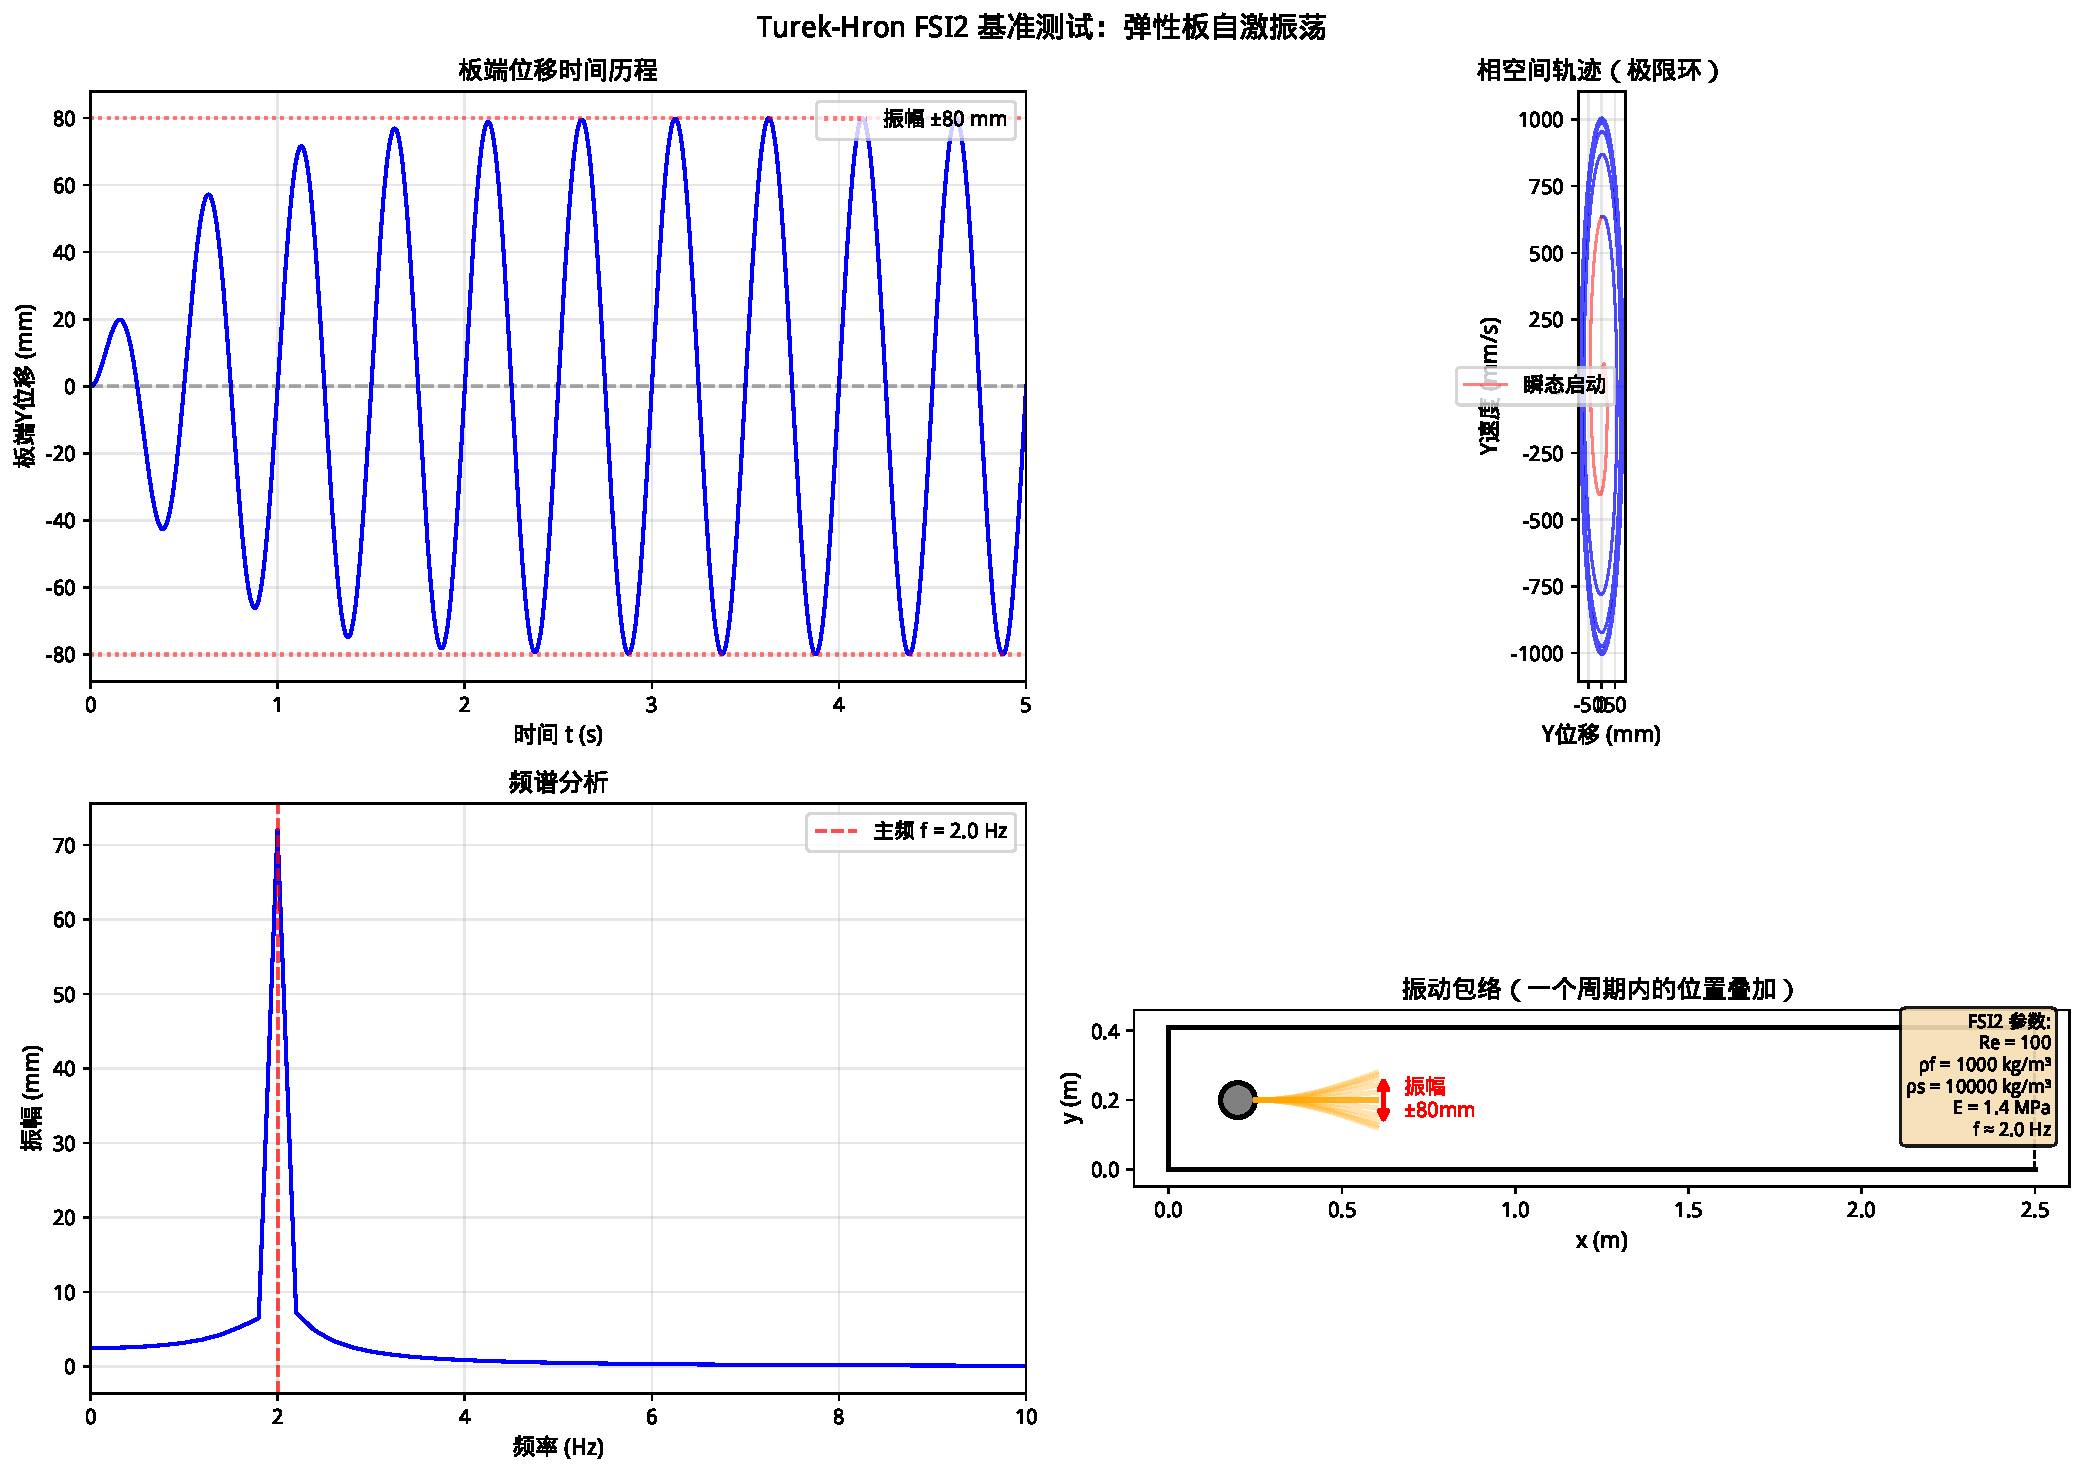
\includegraphics[width=0.98\textwidth]{figs_chap05/turek_fsi2_time_history.pdf}
\caption{Turek-Hron FSI2动力学分析。\textbf{左上}：板端Y位移时间历程，经过短暂瞬态后进入稳态振荡。\textbf{右上}：相空间轨迹，稳态时形成极限环（limit cycle）。\textbf{左下}：频谱分析显示主频约2 Hz。\textbf{右下}：振动包络展示一个周期内板的位置叠加。}
\label{fig:turek_fsi2_analysis}
\end{figure}

\paragraph{涡激振动机理}
为什么弹性板会自发振荡？图\ref{fig:turek_fsi2_mechanism}解释了涡激振动的物理机理：

\begin{figure}[htbp]
\centering
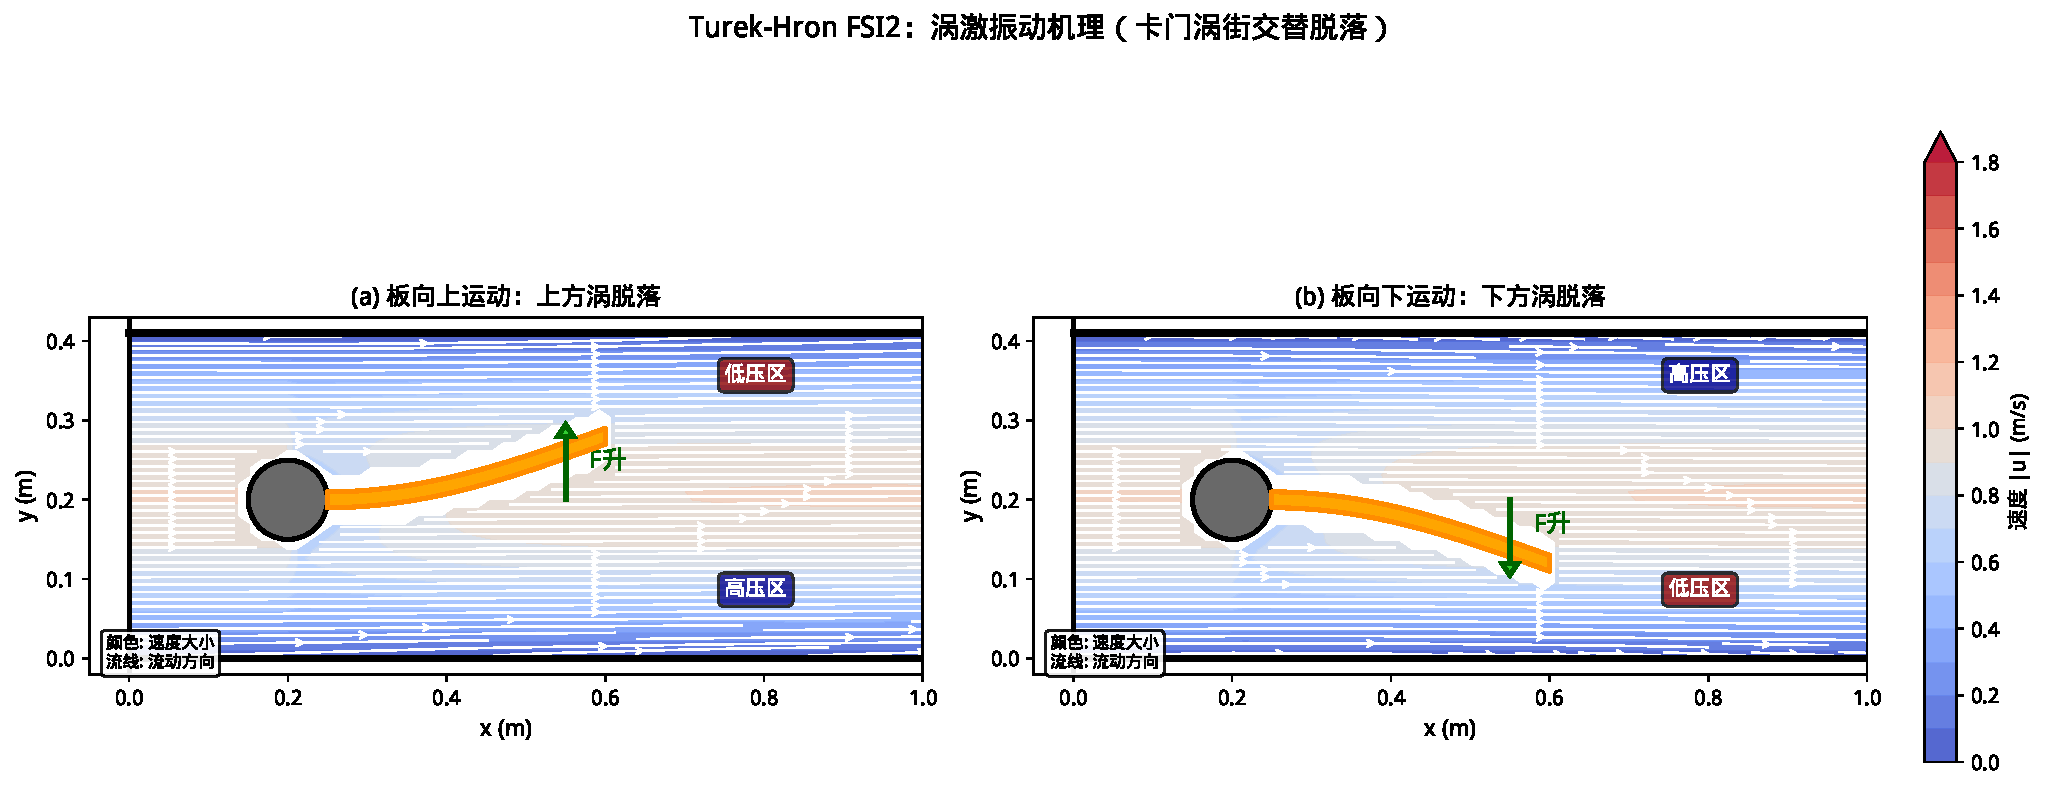
\includegraphics[width=0.98\textwidth]{figs_chap05/turek_fsi2_mechanism.pdf}
\caption{涡激振动机理示意。流体绕过圆柱时形成交替脱落的卡门涡街。(a) 当上方涡脱落时，上方形成低压区，产生向上的升力，推动板向上弯曲。(b) 半个周期后，下方涡脱落，下方形成低压区，产生向下的升力。这种交替的压力差驱动板的周期性振荡。当涡脱落频率接近板的固有频率时，发生\textbf{锁定}（lock-in），振幅达到最大。}
\label{fig:turek_fsi2_mechanism}
\end{figure}

\begin{insightbox}
\textbf{为什么Turek-Hron基准如此重要？}

\begin{enumerate}
    \item \textbf{大变形}：板的位移幅度与板长相当，几何非线性显著
    \item \textbf{强耦合}：固液密度比适中（$\rho_s/\rho_f = 10$），流固相互作用强烈
    \item \textbf{自激振荡}：不是外加强迫振动，而是系统自发产生的不稳定性
    \item \textbf{无实验噪声}：作为数值基准，可以进行严格的代码间比较
\end{enumerate}

如果你的FSI代码能正确重现Turek-Hron基准的结果，那它就有了一定的可信度。
\end{insightbox}

\begin{marginnote}
\textbf{开源实现}：许多开源FSI框架都包含Turek-Hron基准案例，包括：
\begin{itemize}
    \item Kratos Multiphysics
    \item preCICE（耦合库）
    \item Feel++
    \item oomph-lib
\end{itemize}
这些都是学习完整FSI仿真的好资源。
\end{marginnote}

\paragraph{与本节模型的对比}
本节前面的悬臂梁模型（单向耦合、小变形）与Turek-Hron问题（双向耦合、大变形）有本质区别：

\begin{center}
\renewcommand{\arraystretch}{1.3}
\begin{tabular}{l|c|c}
\toprule
& \textbf{本节简化模型} & \textbf{Turek-Hron FSI2} \\
\midrule
流固耦合 & 单向（流$\to$固） & 双向（流$\leftrightarrow$固） \\
变形量级 & 小变形（$w \ll L$） & 大变形（$w \sim L$） \\
流动建模 & 经验公式（Strouhal） & 完整Navier-Stokes \\
计算成本 & 秒级 & 小时/天级 \\
适用场景 & 工程估算、物理直觉 & 精确预测、代码验证 \\
\bottomrule
\end{tabular}
\end{center}

从简化模型到完整的双向耦合FSI，是计算成本增加几个数量级的跨越。但两者并非互斥——简化模型帮助我们建立物理直觉，完整模型用于精确预测和验证。

\begin{references}
\bibitem{turek2006proposal} S. Turek and J. Hron, ``Proposal for Numerical Benchmarking of Fluid-Structure Interaction between an Elastic Object and Laminar Incompressible Flow,'' in \textit{Fluid-Structure Interaction}, Lecture Notes in Computational Science and Engineering, vol. 53, Springer, 2006, pp. 371--385.
\end{references}

